\documentclass[aspectratio=169]{beamer}
\usepackage{graphicx} % Required for inserting images
\usepackage{outlines}
\usepackage{svg}
\usepackage{tikz}
 \usetikzlibrary{calc} 
\usepackage{qrcode}
\usepackage{xcolor}

% ---- Chinese characters --------------------------------------------------------
\usepackage{xeCJK} % for Chinese, compiling by XeLaTex
\usepackage{fontspec} %設定字體
% Fandol font (the default)  not shown "內"
\setCJKmainfont{AR PL UMing TW MBE} % AR PL UMing TW MBE or "UKai" https://www.overleaf.com/learn/latex/Questions/Which_OTF_or_TTF_fonts_are_supported_via_fontspec%3F#Chinese
%BiauKai} %標楷體 from macOS %設定中文為系統上的字型,而英文不去更動,使用原TeX字型

\XeTeXlinebreaklocale "zh"
\XeTeXlinebreakskip = 0pt plus 1pt %這兩行一定要加,中文才能自動換行

%\usepackage{CJKutf8}
%\newcommand{\cntext}[1]{\begin{CJK*}{UTF8}{bkai}#1\end{CJK*}}
%----------------------------------------------------------------------------------------

\usetheme{Warsaw}

\title{Holistic Healthcare from Taiwan Medical Mission \\ in the Republic of Somaliland}

%\title{KOMA_TMM_chief_keynote_20230713_forTMWH}
\author{Dr. Tex Li-Hsing Chi, D.D.S., Ph.D. \\
        Oral and Maxillofacial surgeon \\
        Translational Medicine}
\institute{Taipei Municipal Wanfang Hospital, managed by Taipei Medical University}
\date{5 June 2024} %{13 July 2023}

%%%
\makeatletter
\setbeamertemplate{headline}
{
  \leavevmode%
  \hbox{%
  \begin{beamercolorbox}[wd=.5\paperwidth,ht=2.5ex,dp=1.125ex]{section in head/foot}%
    \insertsectionnavigationhorizontal{.5\paperwidth}{\hskip0pt plus1filll}{}%
  \end{beamercolorbox}%
  \begin{beamercolorbox}[wd=.4\paperwidth,ht=2.5ex,dp=1.125ex,right]{subsection in head/foot}%
    \usebeamerfont{subsection in head/foot}\insertsubsectionhead\hspace*{2ex}
  \end{beamercolorbox}%
  \begin{beamercolorbox}[wd=.1\paperwidth,ht=2.5ex,dp=1.125ex,left]{subsection in head/foot}%
    %\includesvg[height=2.5ex]{TMM_logo.svg}
  \end{beamercolorbox}}%
  \vskip0pt%
}
\makeatother
%%%


%%%
\makeatletter
\setbeamertemplate{footline}
{
  \leavevmode%
  \hbox{%
  \begin{beamercolorbox}[wd=.333333\paperwidth,ht=2.25ex,dp=1ex,center]{author in head/foot}%
    %\usebeamerfont{author in head/foot}\insertshortauthor
    Chief Jamal Tex of TMM
  \end{beamercolorbox}%
  \begin{beamercolorbox}[wd=.333333\paperwidth,ht=2.25ex,dp=1ex,center]{title in head/foot}%
    Holistic Healthcare from TMM
  \end{beamercolorbox}%
  \begin{beamercolorbox}[wd=.333333\paperwidth,ht=2.25ex,dp=1ex,right]{date in head/foot}%
    \usebeamerfont{date in head/foot}\insertshortdate{}\hspace*{2em}
    \insertframenumber{} / \inserttotalframenumber\hspace*{2ex} 
  \end{beamercolorbox}}%
  \vskip0pt%
}
\makeatother
%%%


%%%
\setbeamertemplate{frametitle}
{
    \nointerlineskip
    \begin{beamercolorbox}[sep=0.3cm,ht=1.8em,wd=\paperwidth]{frametitle}
        \vbox{}\vskip-2ex%
        \strut\insertframetitle\strut
        \hfill
        \includesvg[height=1.7em]{TMM_logo.svg}
        \vskip-0.8ex%
    \end{beamercolorbox}
}
%%%

\begin{document}
%\begin{abstract}
%The Taiwan Medical Mission (TMM) is an overseas project that helps the people of Somaliland get health care since 2022/07/28. The TMM is a medical mission that helps people of the people in the Somalia region get medical care. It is also a telepathology project with a pathologist through digital whole-slide images (WSIs). This project supports medical staffs who work at the Hargeisa Group Hospital (HGH) and a hospital in Somalia. This project aims to support medical staff members who work in the HGH. In addition, the TMM supports the health care system in the Taiwan medical mission.
%\end{abstract}

%\begin{CJK*}{UTF8}{gbsn}

\begin{frame}
\titlepage
\end{frame}

\begin{frame}
\frametitle{Outline}

\begin{columns}
\column{0.4\textwidth}
\tableofcontents

\column{0.6\textwidth}
\includesvg[width=0.7\textwidth]{TMM_logo.svg}

\end{columns}


\end{frame}


%%%%%
\section{Overture}

\begin{frame}{序曲}
    \begin{center}
        \includesvg[width=0.8\textwidth]{TRO_Somaliland_font_ZongKai.svg}
    \end{center}
\end{frame}

\begin{frame}{序曲}

\begin{columns}
\column{0.4\textwidth}
    \begin{outline}
        這裡是外交先鋒,\\
        這裡是戰地後盾,\\
        這裡是,1973年代的臺灣,\\
        我們沒有參與過去的臺灣,\\
        但我們正在撰寫索蘭的醫療史,\\
        Taiwan Medical Mission 是,\\
        不拿槍的幕後英雄。\\
    \end{outline}

\column{0.6\textwidth}
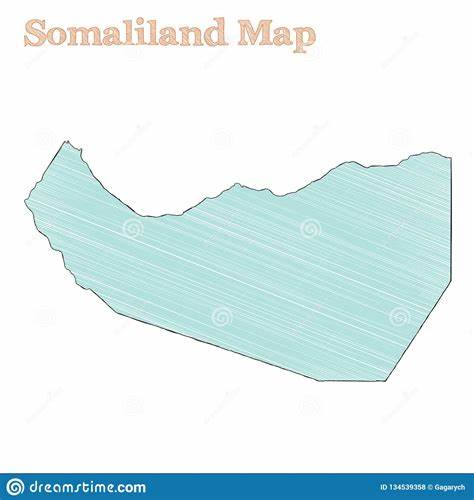
\includegraphics[width=0.7\textwidth]{Somaliland.jpeg}
\end{columns}

\end{frame}




%%
\section{Q\&A 2023}
%\documentclass{beamer}
%\usepackage{CJKutf8}
%\usepackage{hyperref}


\begin{frame}
\frametitle{月梅高 15:06}
%\begin{CJK}{UTF8}{bsmi}
這麼多年,有其他國家與你們合作嗎?
%\end{CJK}

%\begin{CJK}{UTF8}{bsmi}
答:我們醫療團會在駐地,與英、美、澳洲等 NGO 合作推動計畫。
%\end{CJK}
\end{frame}

\begin{frame}
\frametitle{黃森愛 15:07}
%\begin{CJK}{UTF8}{bsmi}
請問祁醫師其他國家給予什麼樣的協助對於索馬利蘭的醫療發展是有幫助的?
%\end{CJK}

%\begin{CJK}{UTF8}{bsmi}
答:同上,例如肝炎疫苗、UNICEF婦幼保健、安全用水,今年度(2024)我們醫療團則推行登革熱及瘧疾防治工作,以及子宮頸抹片檢查 6分鐘護一生。
%\end{CJK}
\end{frame}

\begin{frame}
\frametitle{黃亭榕 15:10}
%\begin{CJK}{UTF8}{bsmi}
請問祁醫師覺得台灣在醫療的哪一方面還能提供更多什麼幫助
%\end{CJK}

%\begin{CJK}{UTF8}{bsmi}
答:全面都行。而目前先由婦幼、骨科、外科開始,以及肝炎疫苗、登革熱、子宮頸HPV疫苗。
但是,有些手術在臺灣已經看不到了,倒是我們要向他們學習(先天性唇顎裂、無肛門症、槍傷,非常困難的生產)
%\end{CJK}
\end{frame}

\begin{frame}
\frametitle{潘星宇 15:10}
%\begin{CJK}{UTF8}{bsmi}
想問索馬利蘭這個國家治安相較於其他國家好嗎?
%\end{CJK}

%\begin{CJK}{UTF8}{bsmi}
答:相對安全(與南非、中美洲比)
%\end{CJK}
\end{frame}

\begin{frame}
\frametitle{吳芊慧 15:11}
%\begin{CJK}{UTF8}{bsmi}
請問祁醫師您覺得有什麼樣特質的人或有什麼資歷可以到非洲醫療團?
%\end{CJK}

%\begin{CJK}{UTF8}{bsmi}
答:有愛心、同理心、愛交朋友,能隨遇而安,而且若沒有(亞洲)臺灣食物就算了。
%\end{CJK}
\end{frame}

\begin{frame}
\frametitle{紀馥蓉 15:13}
%\begin{CJK}{UTF8}{bsmi}
請問祁醫生在那邊的生活會不會有不適應的地方?
%\end{CJK}

%\begin{CJK}{UTF8}{bsmi}
答:2022/07 抵達時:哇怎麼都是石頭路與沙地,柏油路少見,也滿佈坑洞。\\
(Dr. Andrew: 都沒有冷氣機,中午好熱....35 degree C)
%\end{CJK}
\end{frame}

\begin{frame}
\frametitle{彭于庭 15:14}
%\begin{CJK}{UTF8}{bsmi}
想問祁醫生,對以後有想去當國際醫療志工的人有沒有什麼建議,例如:需要先具備良好得醫學知識等?
%\end{CJK}

%\begin{CJK}{UTF8}{bsmi}
答:學生團體就能開始累積國際經驗,外交替代役男是個好主意,至於醫療團,要等到護理師、專科醫師有經驗之後囉。英語的聽說寫很重要。
%\end{CJK}
\end{frame}




%%
\section{Introduction}
\begin{frame}
\frametitle{Introduction}
% Add content here
\begin{outline}
    

\1 The Taiwan Medical Mission (TMM) is an overseas project that helps the people of Somaliland get health care since 2022/07/28.
    \2 our brother mission: TMM in the Kingdom of Eswatini since 2008 leaded by Dr. Tu Chi-cheng (杜繼誠團長)
\1 The team consists of % 程書螢 林威霖 巫昀祐 黃郁昕
    \2 an obstetrician (YuHsin), a registered nurse (Penny), a general surgeon doctor (Andrew), and an oral and maxillofacial surgeon (Jamal Tex); a administrator (Amui). 
    \2 to support medical staffs who work at the Hargeisa Group Hospital (HGH), Hargeisa, Somaliland
%\1 TMM members are willing to adapt to different cultures and settings and work with limited resources and facilities.



\end{outline}

\qrcode[height=0.7in]{https://youtu.be/uOwzikPw-0U}
2023/05 消失的國界(三立電視 東非現場)

\end{frame}


\begin{frame}{Medical affairs - 消失的國界}
    \begin{center}
        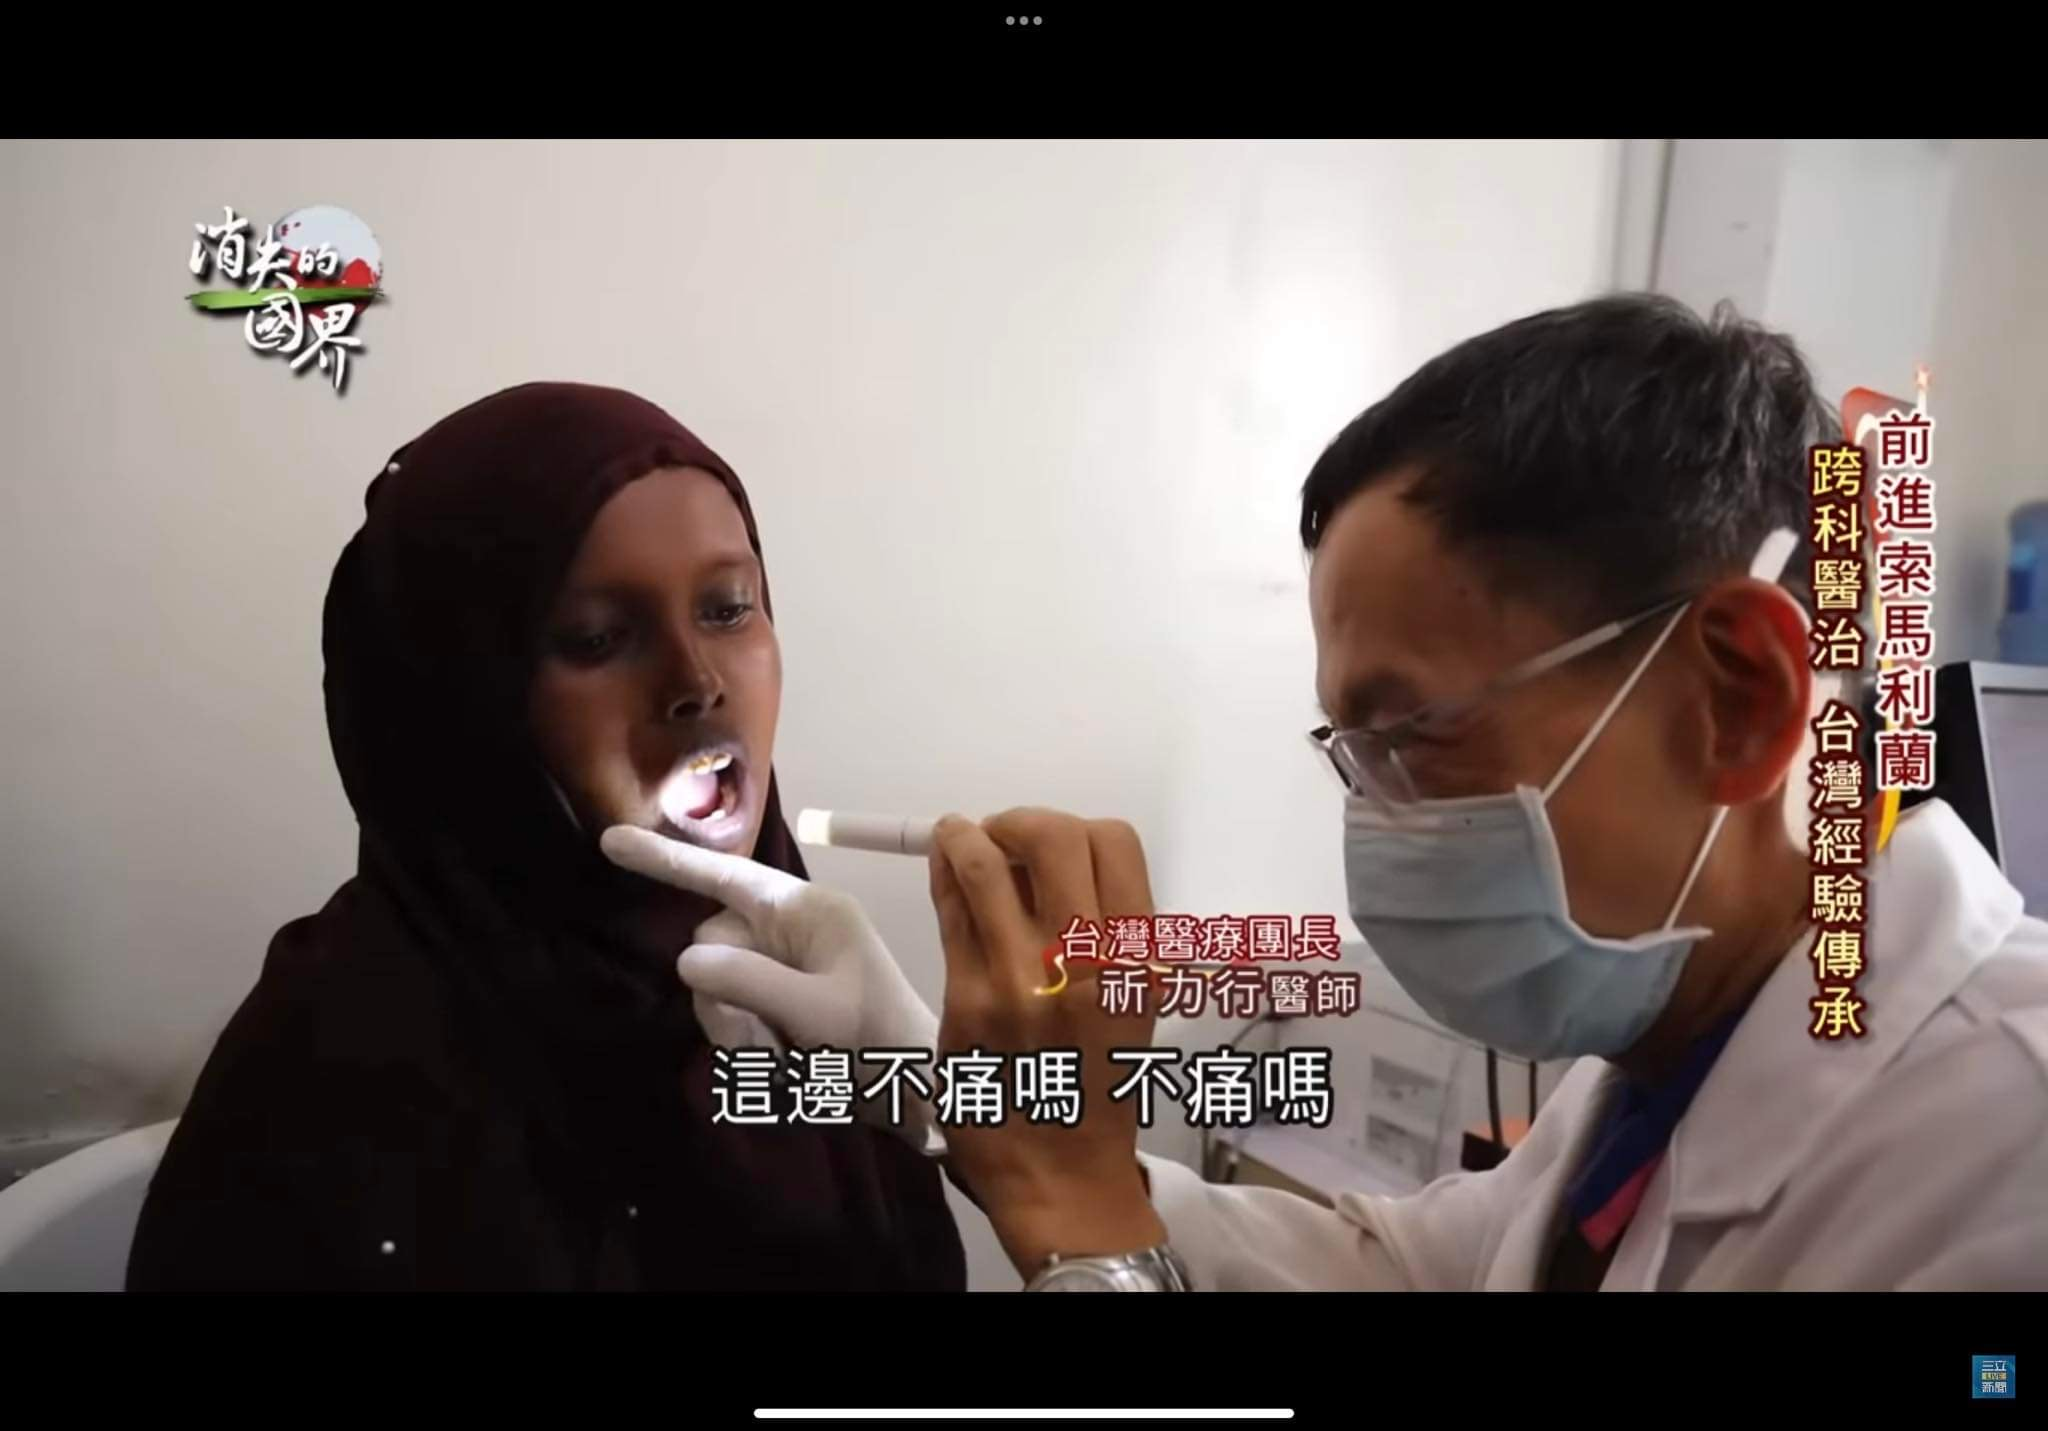
\includegraphics[width=0.8\textwidth]{IMG_4940(1).jpeg}

    \end{center}
\end{frame}

\begin{frame}{Medical affairs - 消失的國界}
\begin{center}
    
\begin{tikzpicture}
    \node[anchor=south west,inner sep=0] (image) at ($(current page.center)+(-2cm,0)$) {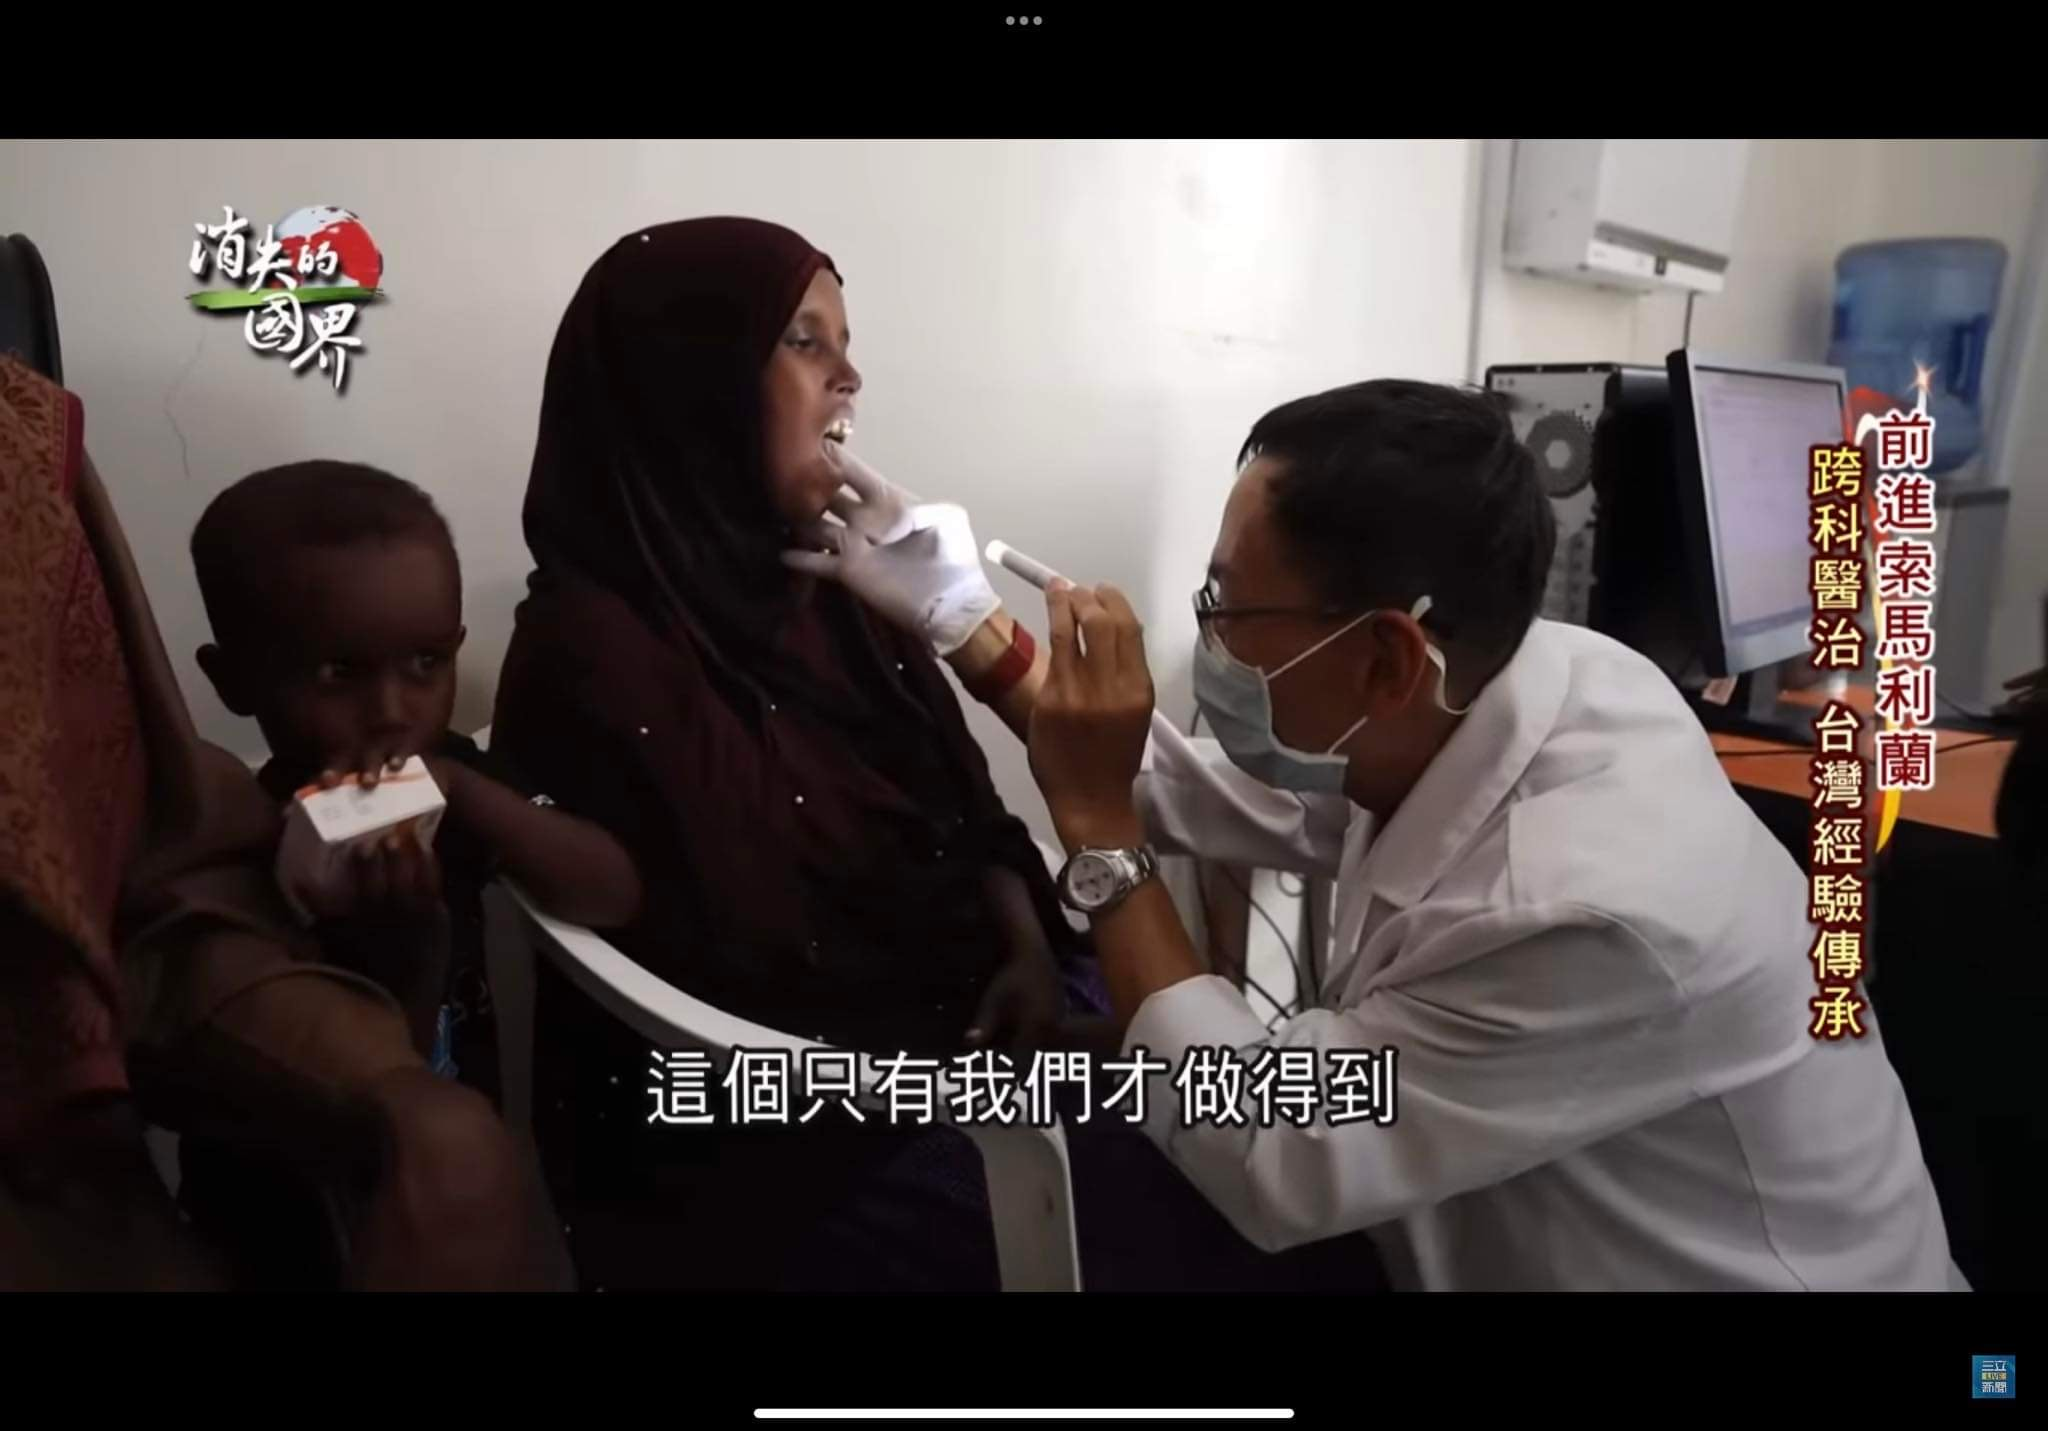
\includegraphics[width=0.8\textwidth]{IMG_4949(1).jpeg}};
    \begin{scope}[x={(image.south east)},y={(image.north west)}]
        \fill[white] (0.25,0.60) circle (0.04);
    \end{scope}
\end{tikzpicture}

\end{center}

\end{frame}


\begin{frame}{Two TMMs in the World}
\begin{tikzpicture}
\node[anchor=west] (africa) at (0,0) {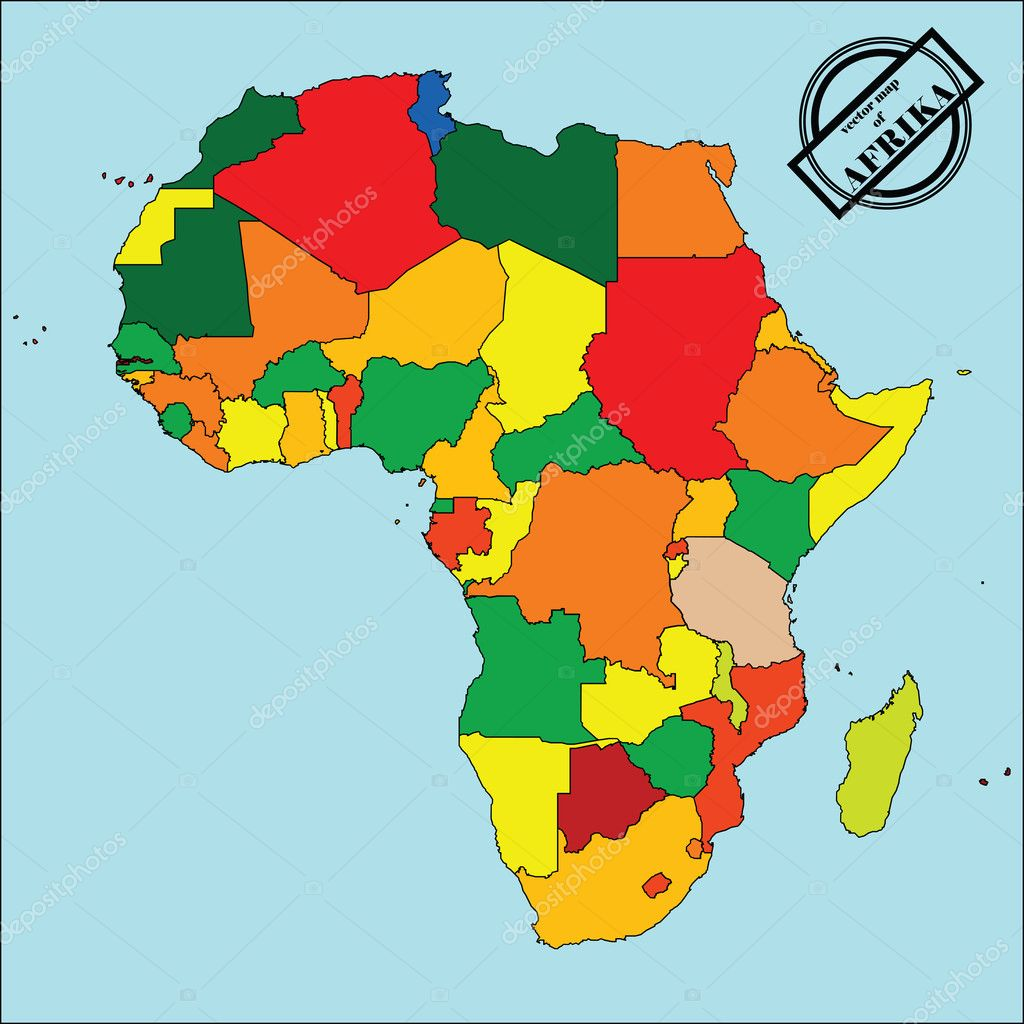
\includegraphics[width=0.4\textwidth]{worldMap_Africa.jpeg}};

\node[anchor=south west] (TMM_2022) at ([yshift=+2.0cm]africa.east) {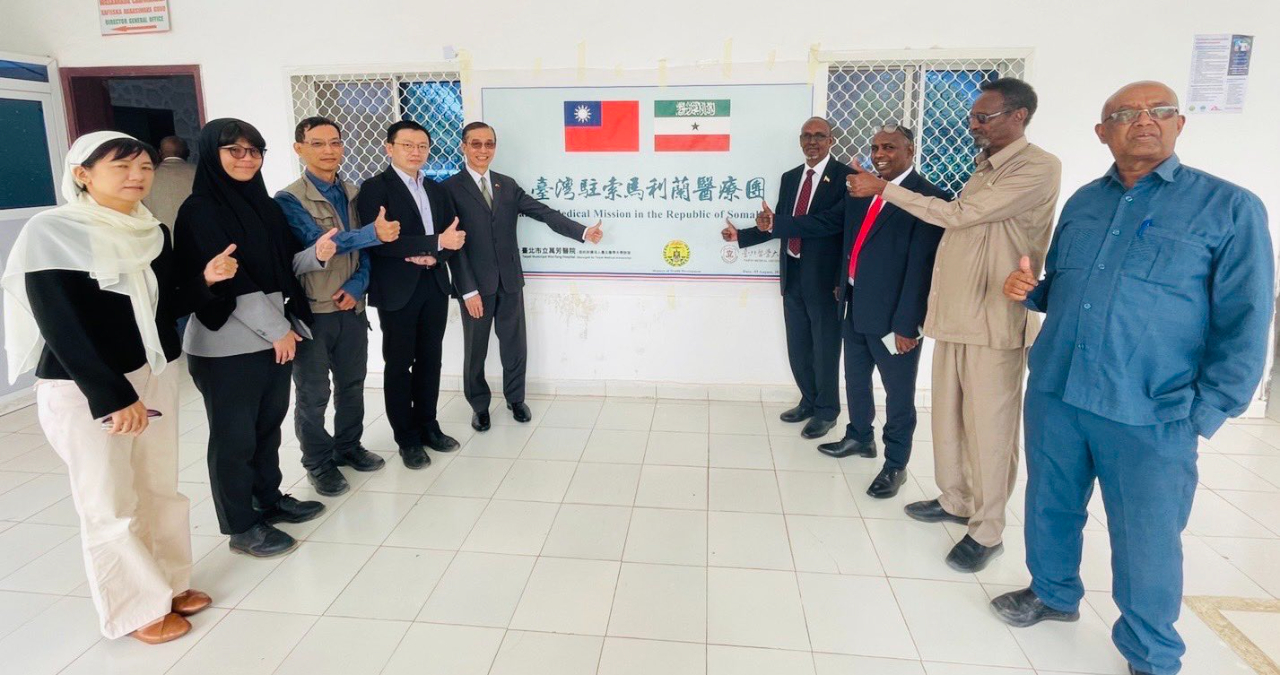
\includegraphics[width=0.30\textwidth]{TMM2022July.jpeg}};

\node[anchor=south west] (TMM_sln) at ([xshift=+4.5cm, yshift=+0.8cm]africa.east) {\includesvg[width=0.14\textwidth]{TMM_logo.svg}};
\node[anchor=west] at (TMM_sln.east) {2022/July};
\draw[green,thick,<-] (4.9,0.55) -- (10.7,1.4);

\node[anchor=north west] (TMM_swati) at ([xshift=+2.0cm, yshift=+0.5cm]africa.east) {
\includegraphics[width=0.15\textwidth]{TMM_Eswatini_logo.jpg}};
\node[anchor=west] at (TMM_swati.east) {2008/Sep};
\draw[blue,thick,<-] (3.95,-1.8) -- (8.2,-1.0);
%\draw (africa.east) -- (TMM_swati.west);
\end{tikzpicture}
\end{frame}



\begin{frame}{Islamic Africa}

\begin{outline}
    \1 TMM members are willing to adapt to Muslim's cultures and settings and work with limited resources and facilities.

\end{outline}

\begin{center}

\includegraphics[width=0.23\textwidth]{IMG_4872.jpeg}
\includesvg[width=0.14\textwidth]{anti_CervicalCancer_logo.svg}
\includesvg[width=0.23\textwidth]{Muslim_women_1.svg}
%\includesvg[width=0.14\textwidth]{Muslim_women_2.svg}
%\includesvg[width=0.2\textwidth]{parasite_logo.svg}
\end{center}

\end{frame}
%%%%%%%%%%%%%%%%%%%%%%%%%
\section{Projects}
\begin{frame}
\frametitle{2023 TMM's Projects - first pillar}
% Add content here
\begin{outline}
    TMM is working on a number of projects to improve health care by 1) building capacity, 2) upgrading equipment, 3) implementing screening programs, and 4) working with local health workers and organizations to handle medical affairs.
    
    \1 medical affairs
        \2 Providing quality care to patients through referring to the specialists at TMM
        \2 Working on non-communicable diseases (NCD, such as hypertension, diabetes) together with NGOs
        \2 The point-of-care ultrasound in the emergency department and intensive care unit (ICU) of HGH

\end{outline}



\end{frame}

\begin{frame}{Medical affairs - trauma ward}
    \begin{center}
        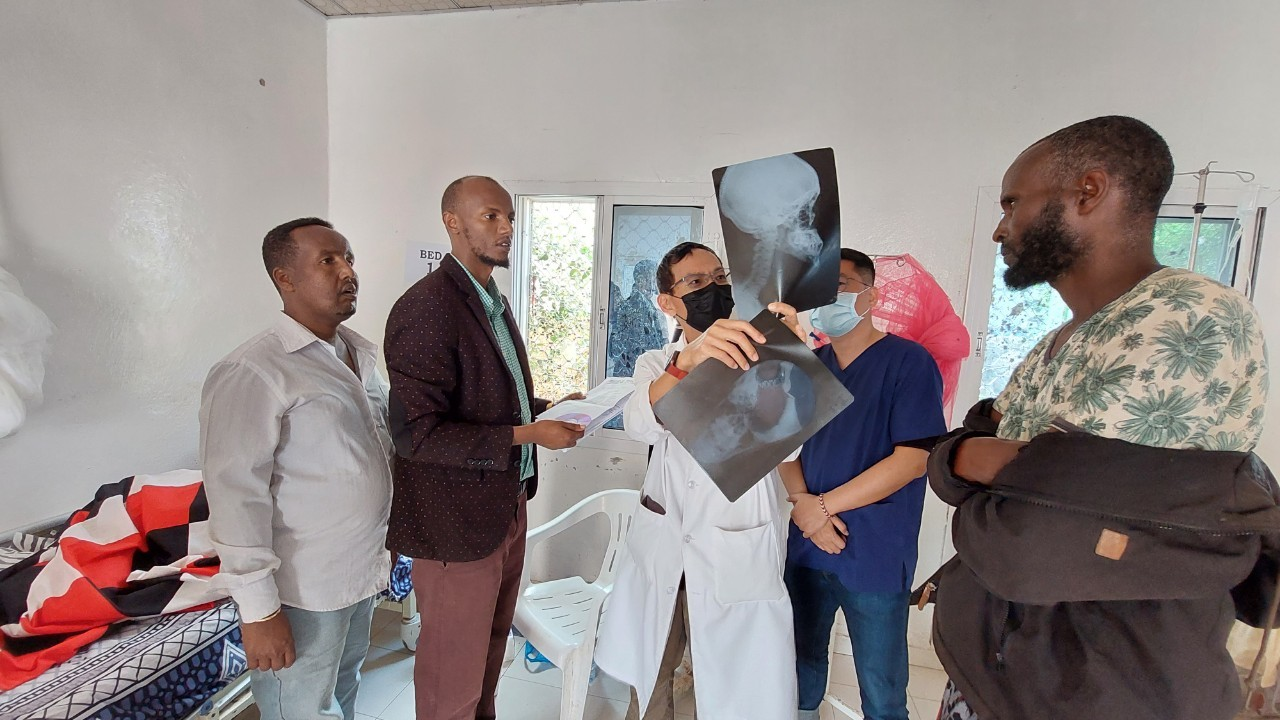
\includegraphics[width=0.8\textwidth]{IMG-4862827583386425169.de8939a35ce768375740b709dce51958.23032108.JPG}
%        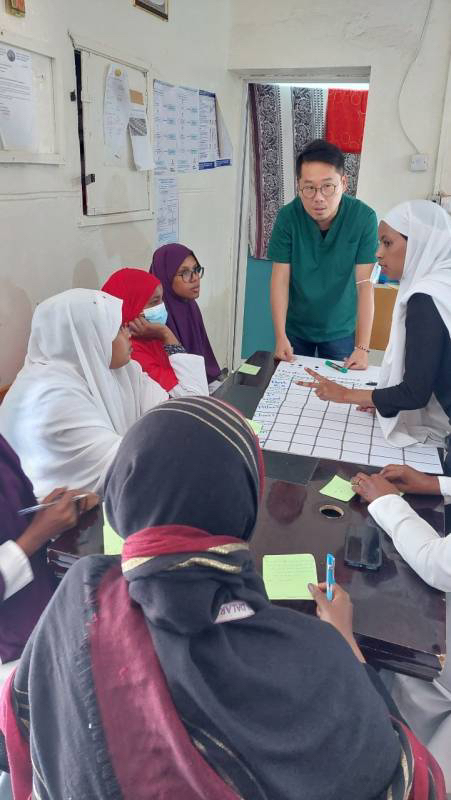
\includegraphics[width=0.2\textwidth]{6963.jpg}
    \end{center}
\end{frame}
    
\begin{frame}{Medical affairs - operation theatre}
    \begin{center}
        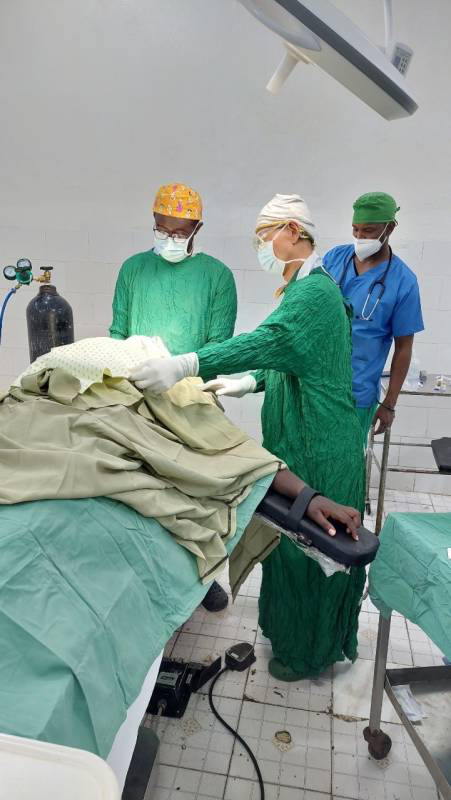
\includegraphics[width=0.35\textwidth]{51744_old_table.jpg}
%        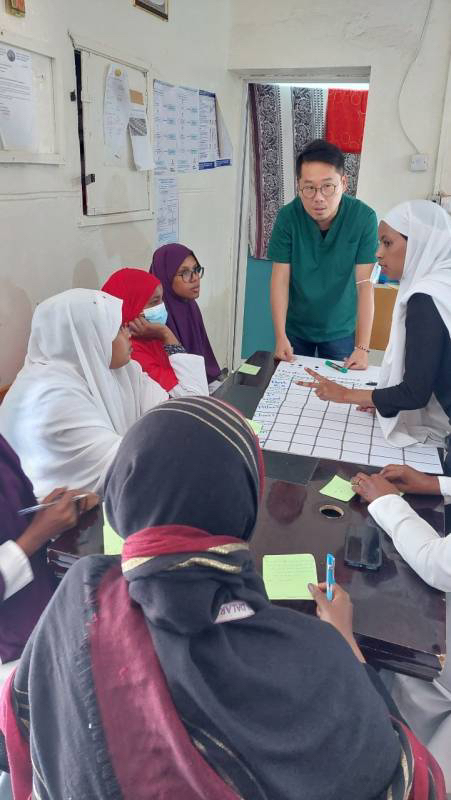
\includegraphics[width=0.2\textwidth]{6963.jpg}
    \end{center}
\end{frame}


\begin{frame}{Medical affairs - OBS, ED}
    \begin{center}
        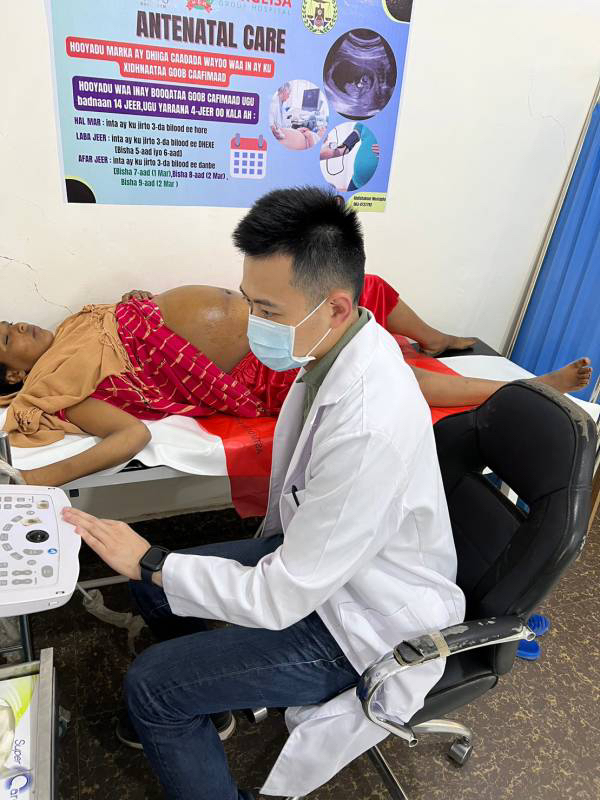
\includegraphics[width=0.25\textwidth, trim=50mm 20mm 40mm 50mm, clip]{52165_antenatal_check.jpg}
        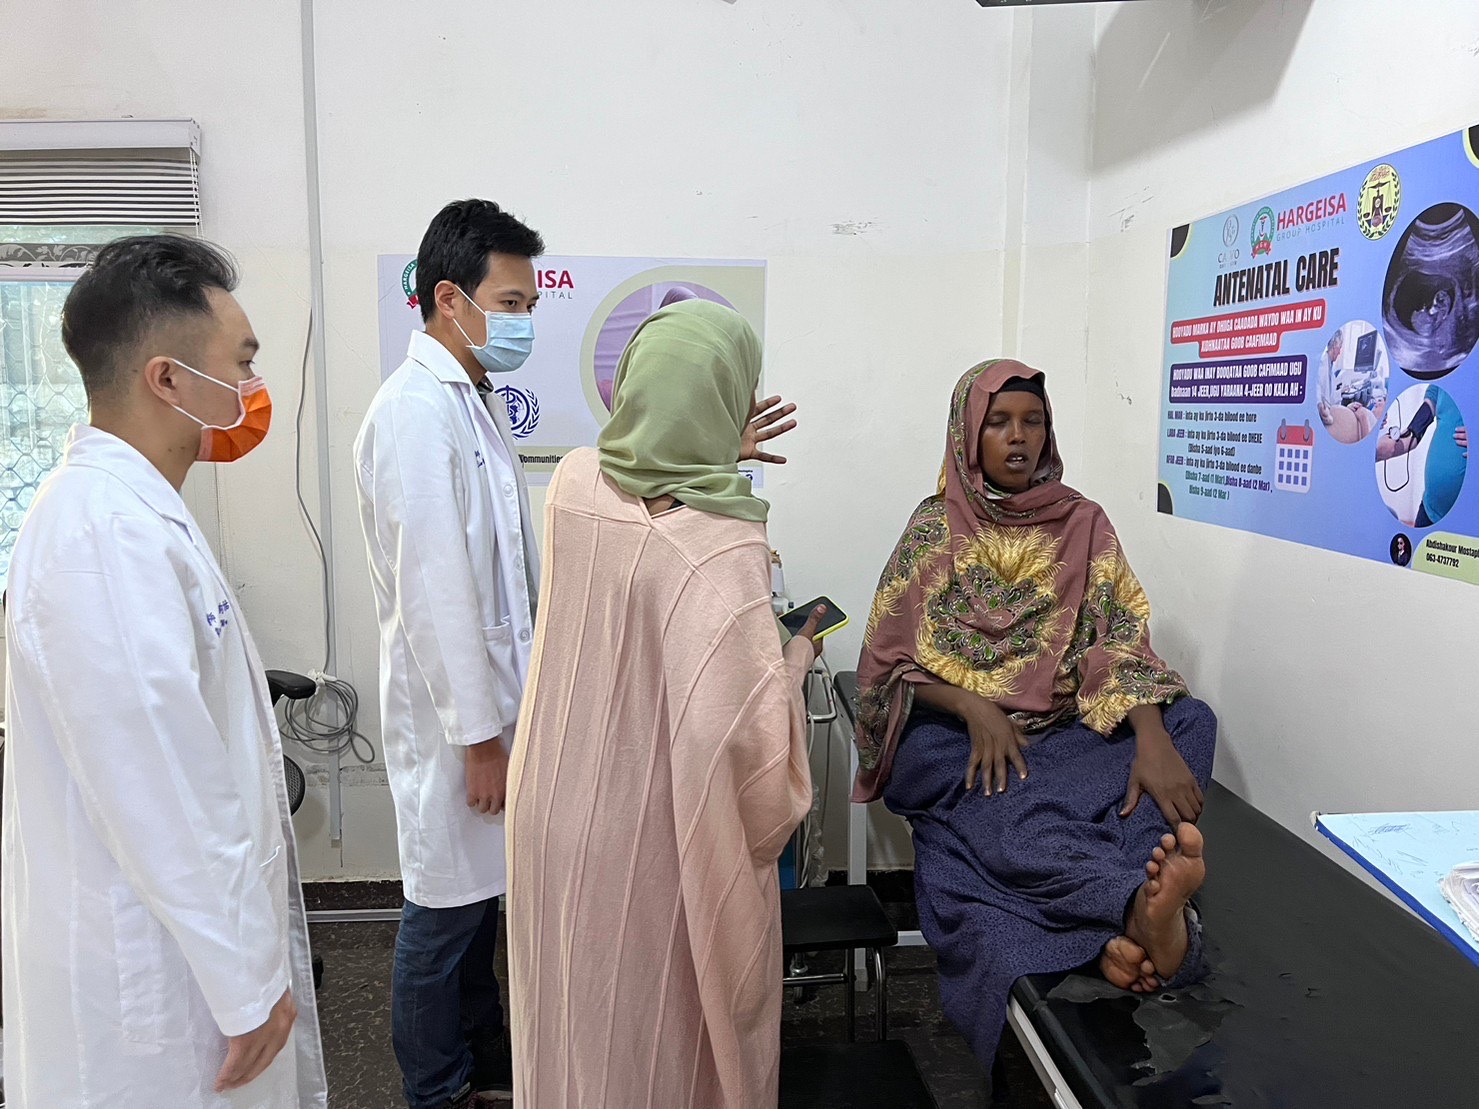
\includegraphics[width=0.4\textwidth]{IMG_5068.jpeg}
    \end{center}
\end{frame}

\begin{frame}{Medical affairs - ED, ward}
\begin{center}
\begin{tikzpicture}
    \node[anchor=south west,inner sep=0] (image) at ($(current page.center)+(0cm,-2cm)$) {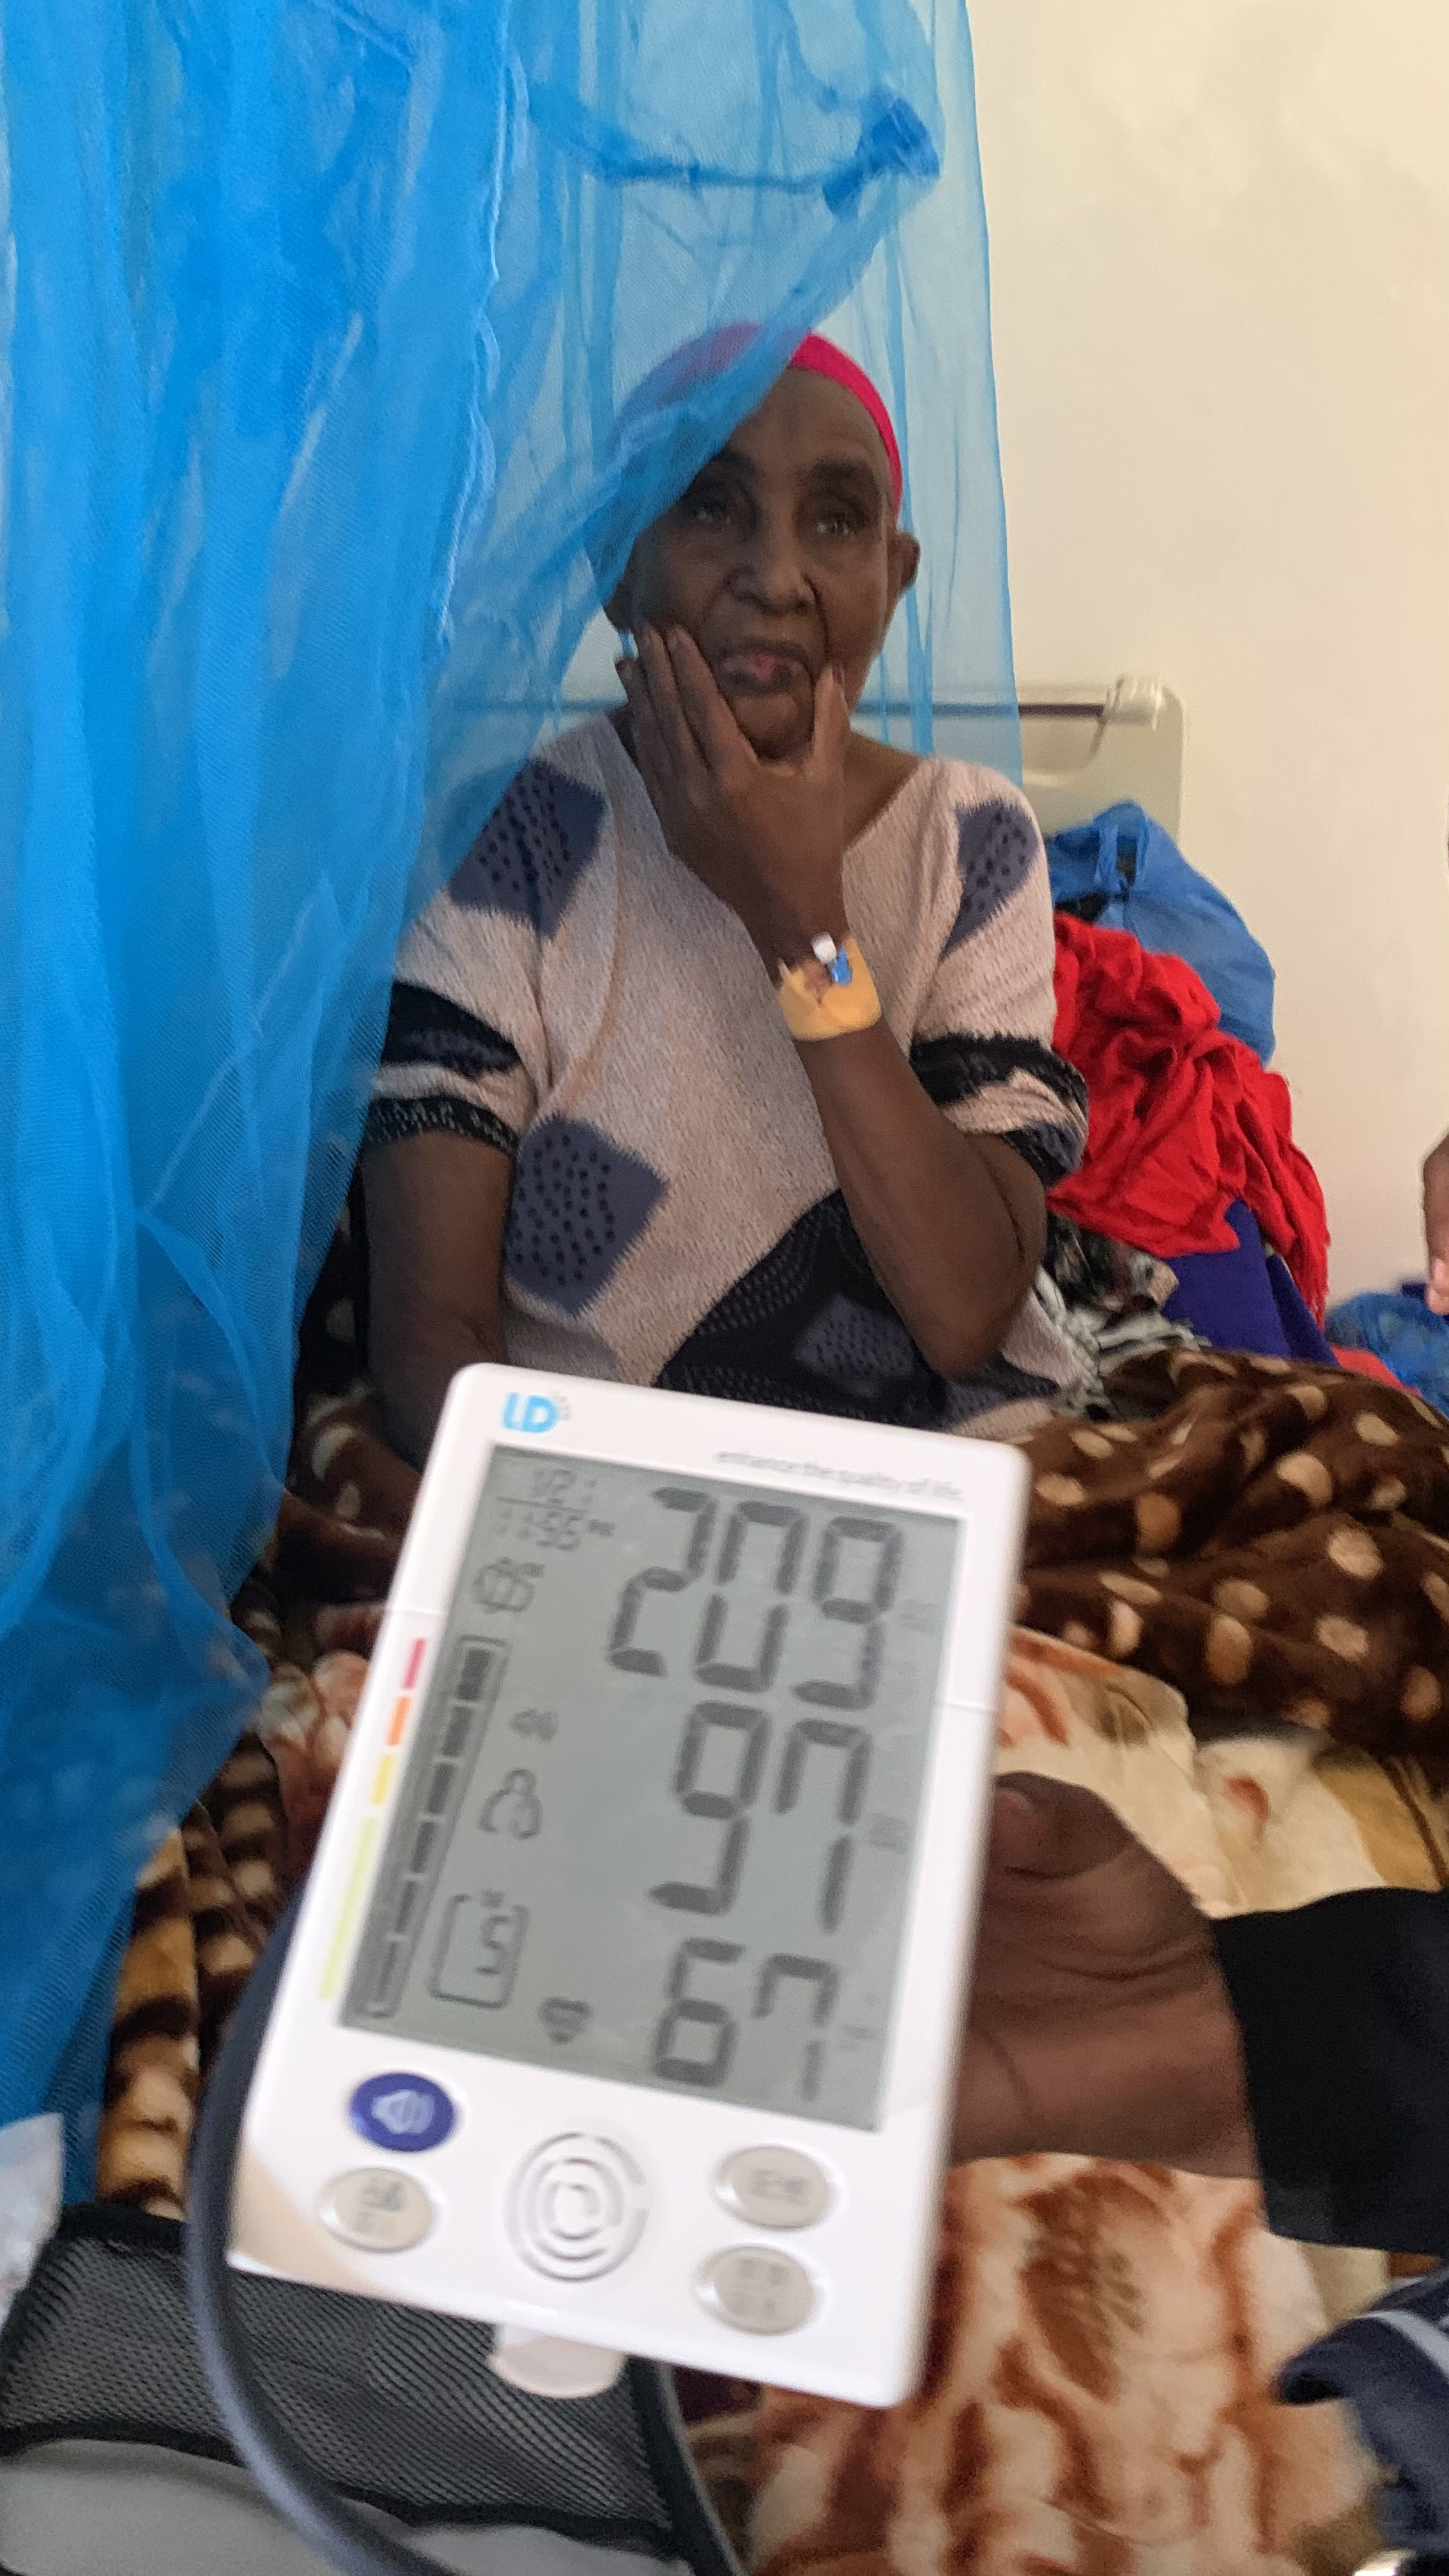
\includegraphics[width=0.30\textwidth]{IMG_5011.jpeg}};
    \begin{scope}[x={(image.south east)},y={(image.north west)}]
        \fill[white] (0.35,0.75) circle (0.03);
    \end{scope}
\end{tikzpicture}

\end{center}
\end{frame}


\begin{frame}{Home visits - OBS, ED}
    \begin{center}
        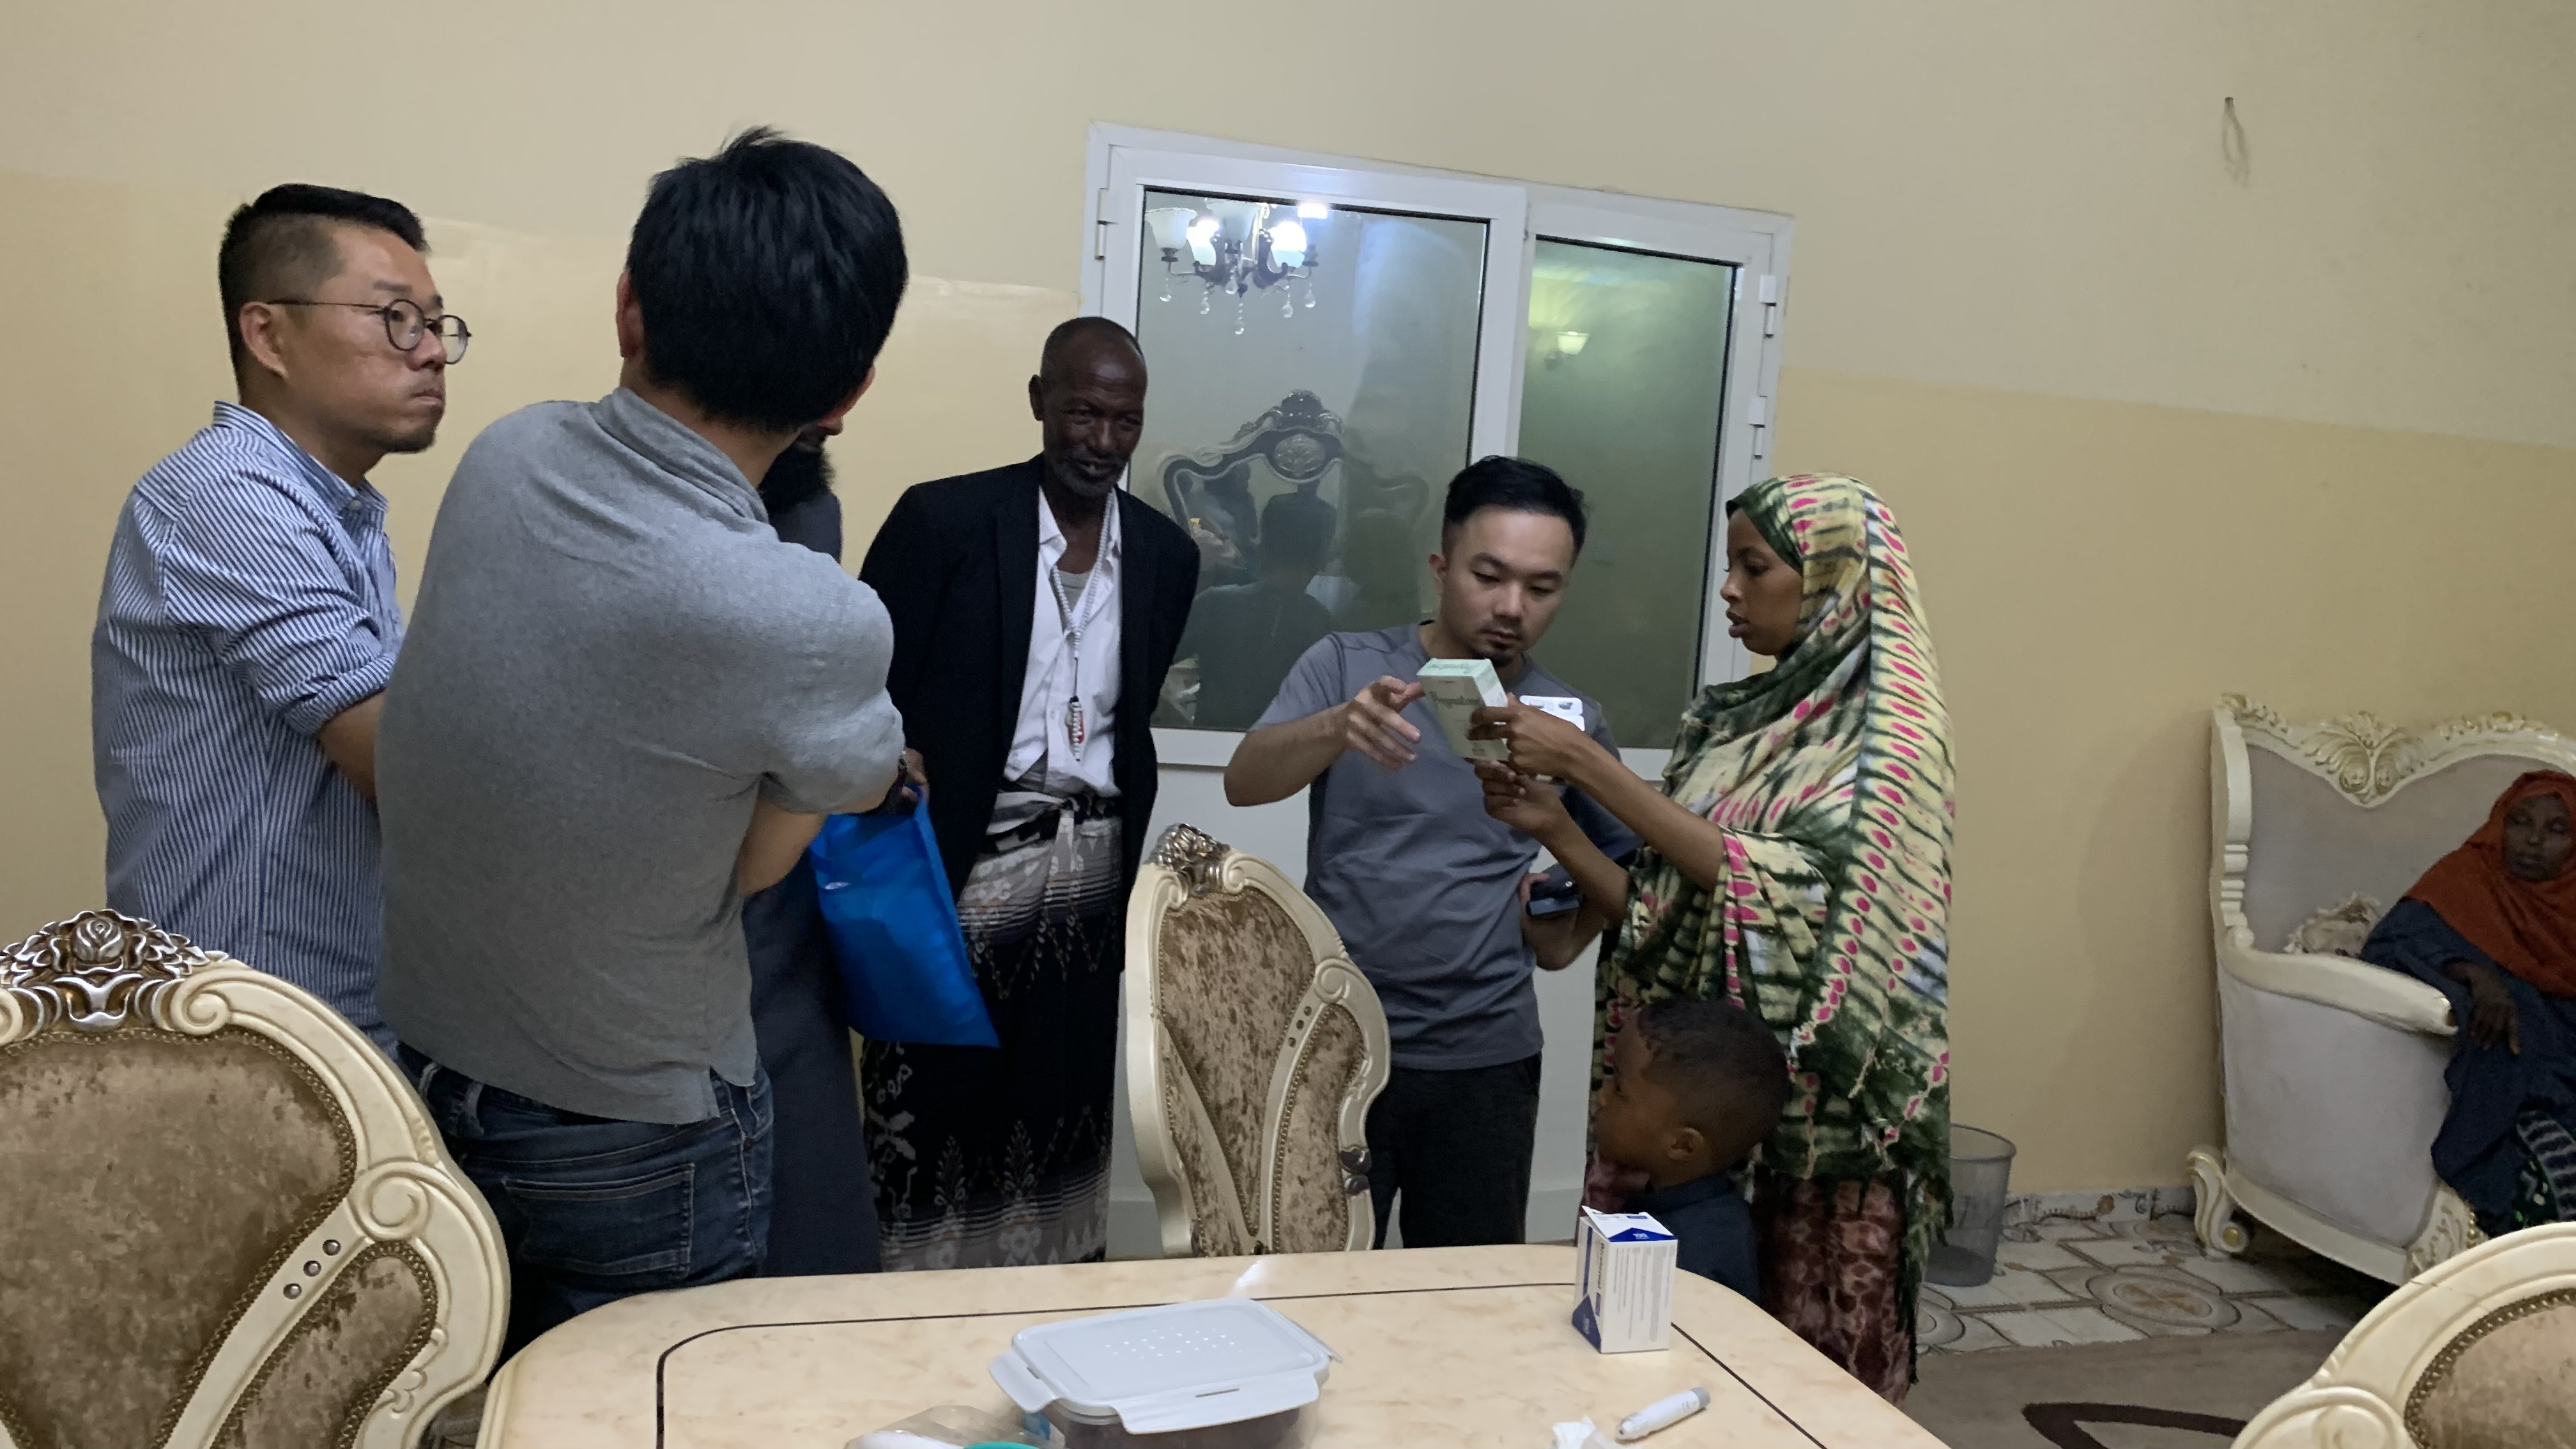
\includegraphics[width=0.55\textwidth]{IMG-5075.jpg}
        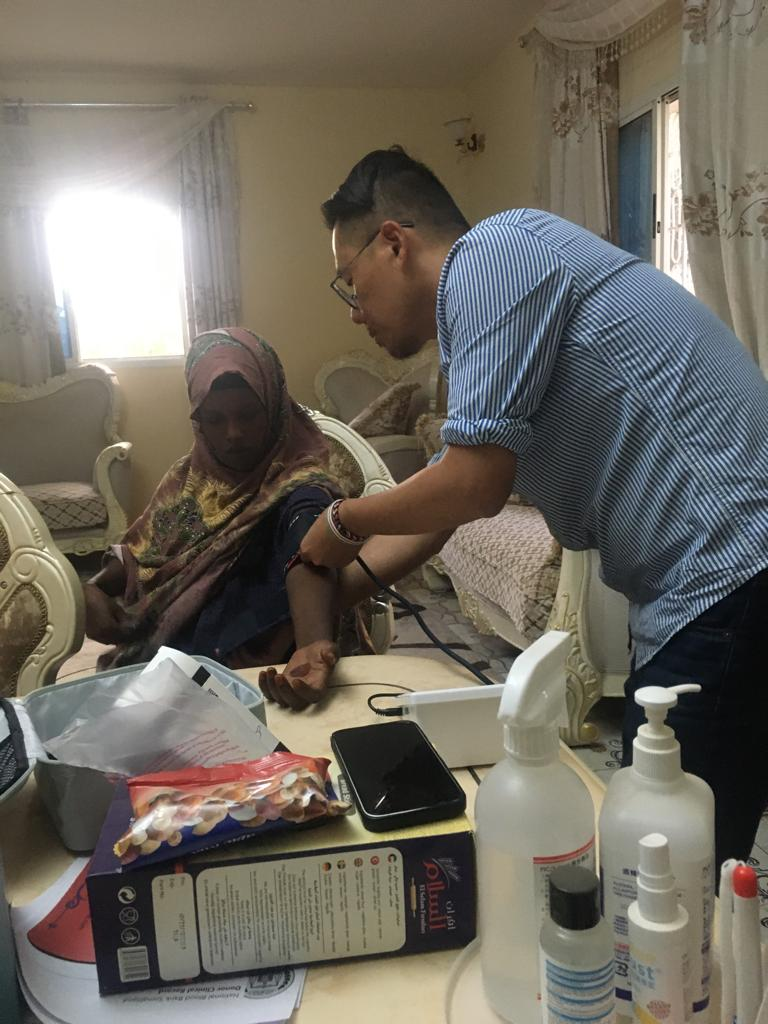
\includegraphics[width=0.25\textwidth]{386eb640-9657-4b71-af5c-5de19cb7b159.JPG}
    \end{center}
\end{frame}


\begin{frame}{Home visits - OMS}
    \begin{center}
        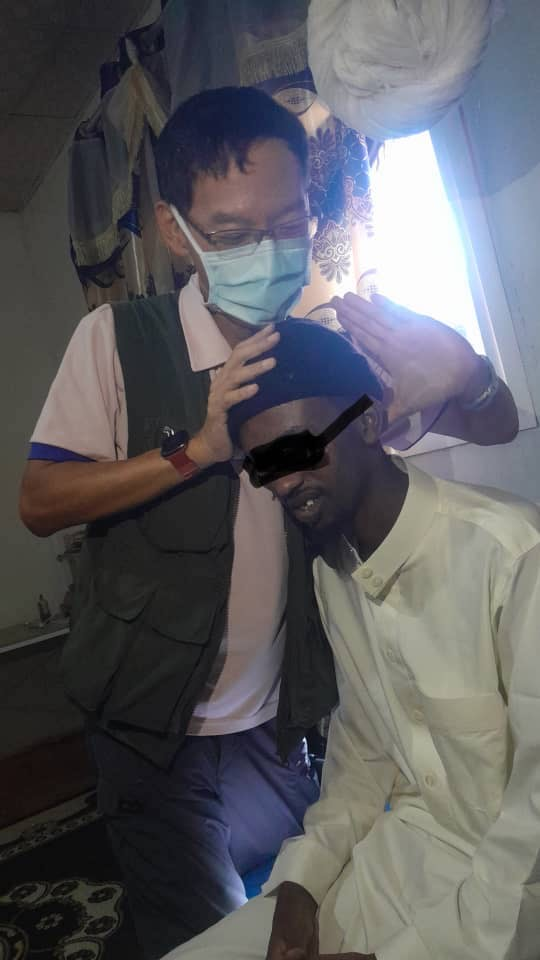
\includegraphics[width=0.20\textwidth]{399223ed-f871-41f7-ae57-c90a5f0ee459.jpeg}
        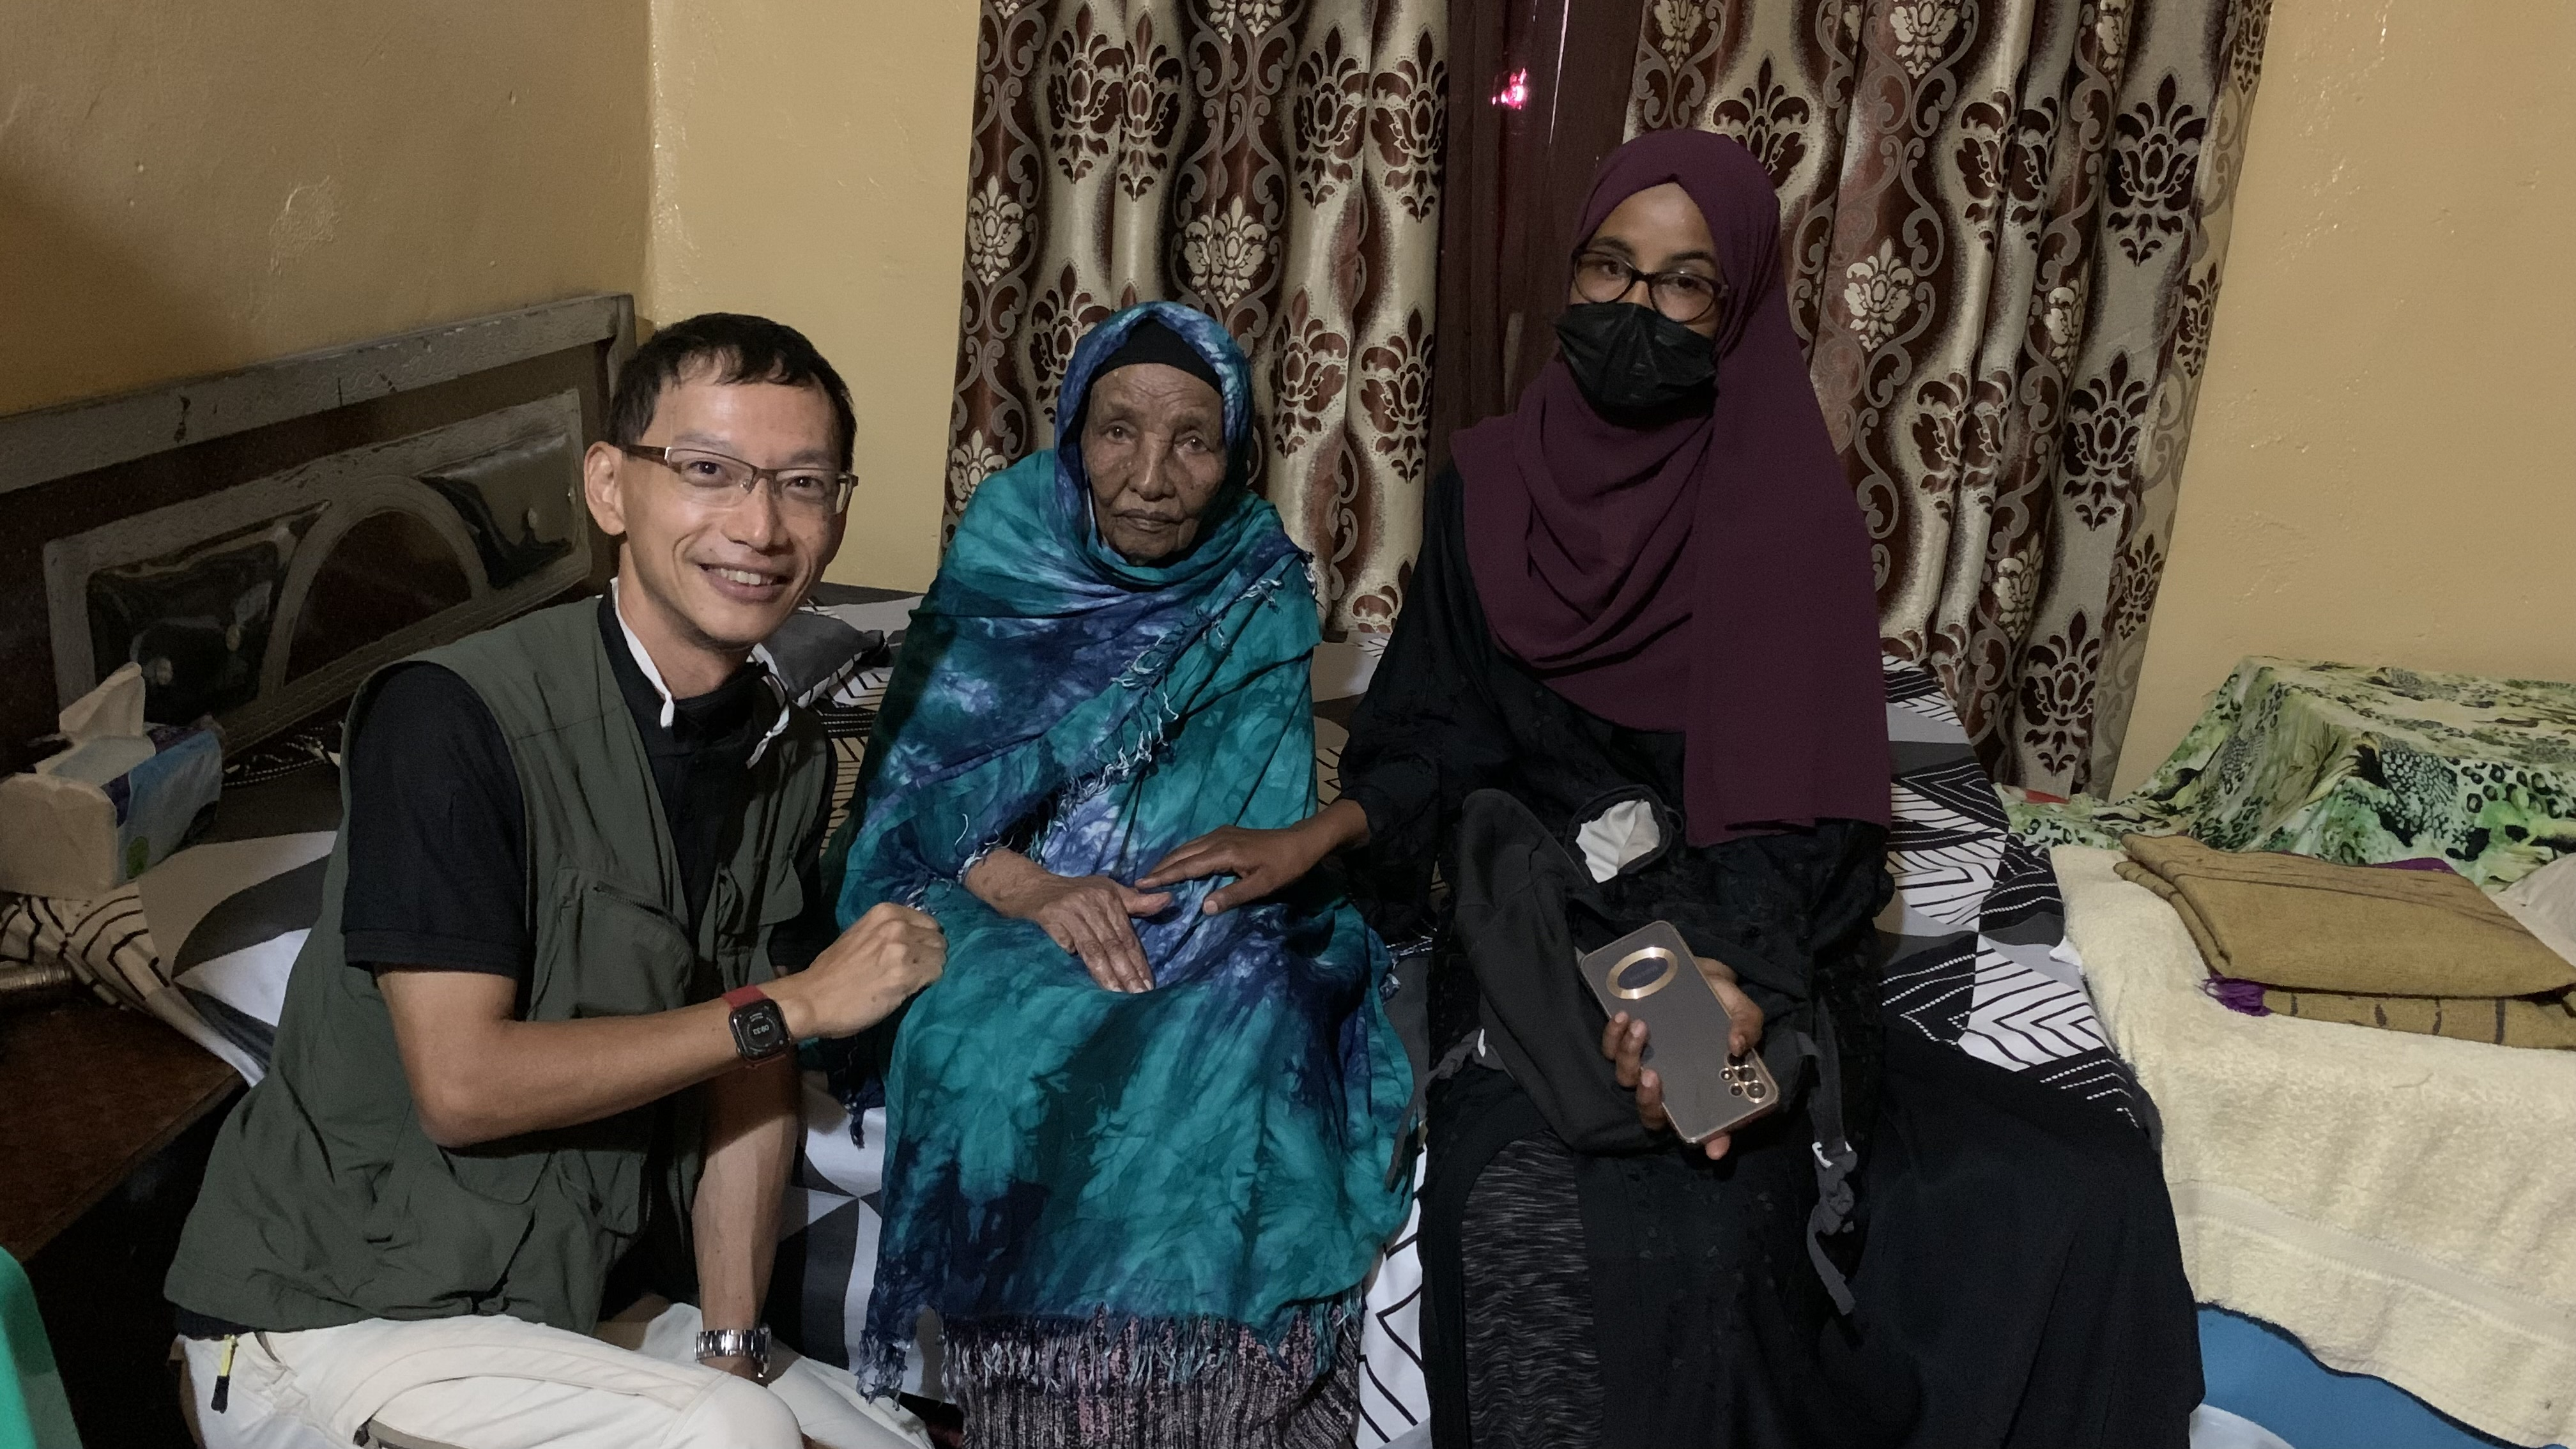
\includegraphics[width=0.50\textwidth]{IMG-3330.jpg}
    \end{center}
\end{frame}




\begin{frame}{Home visits - when doctor becomes patient}
    \begin{center}
        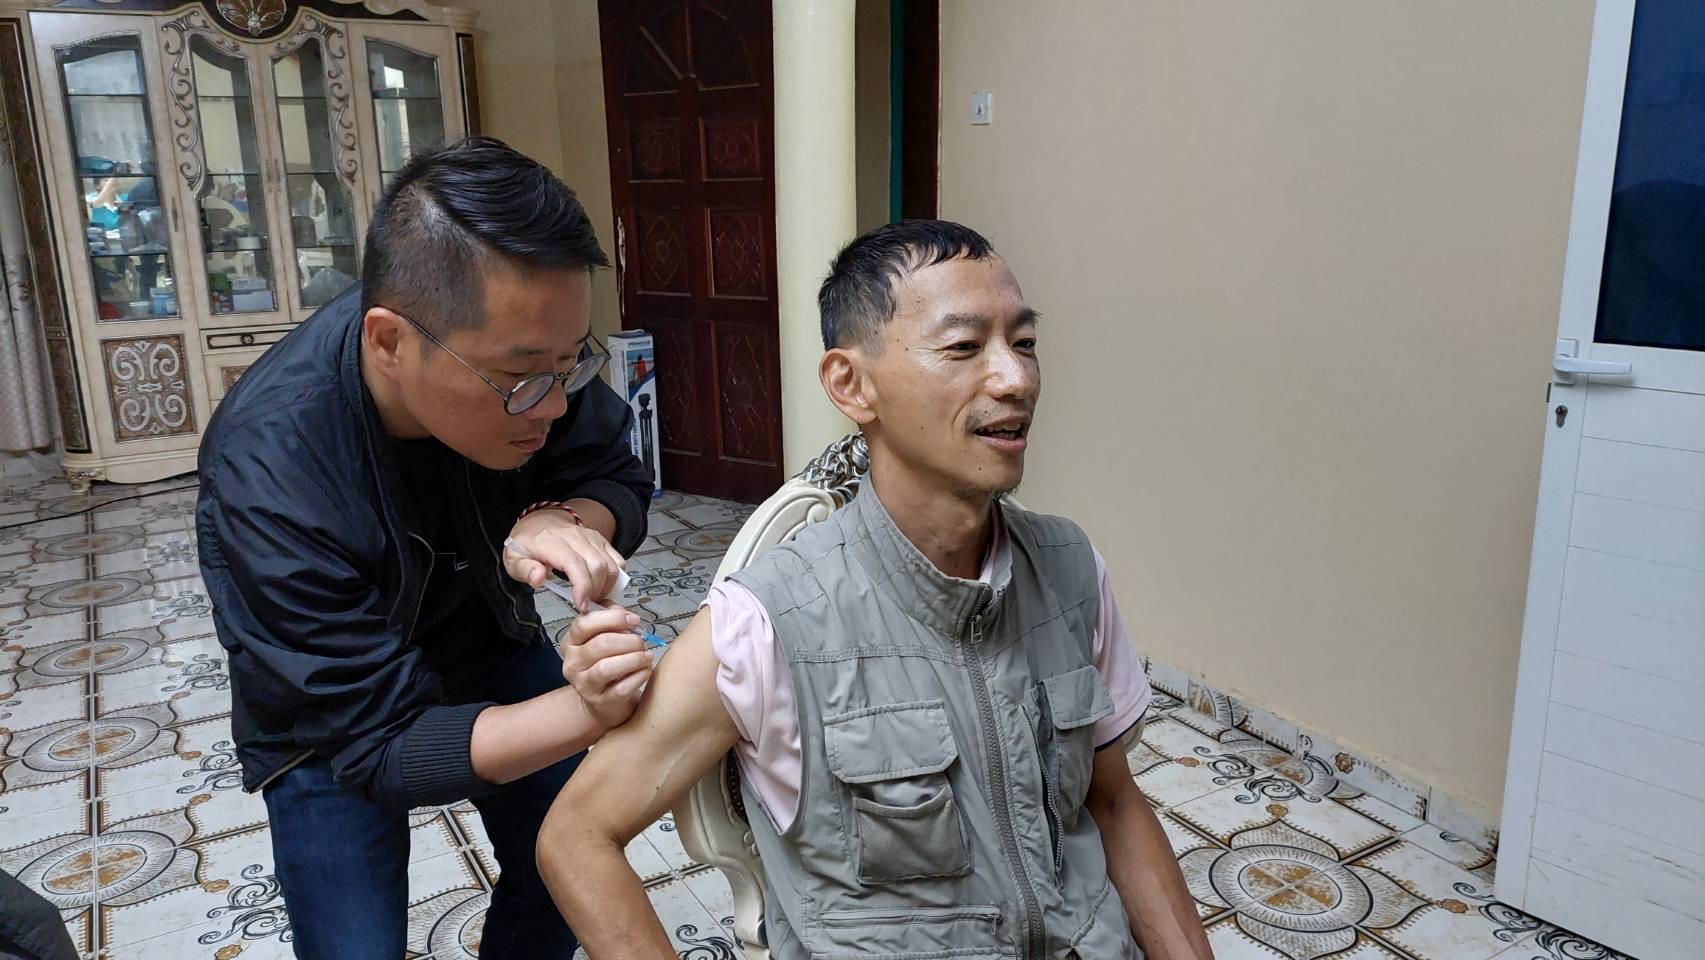
\includegraphics[width=0.50\textwidth]{IMG-2343.JPG}
        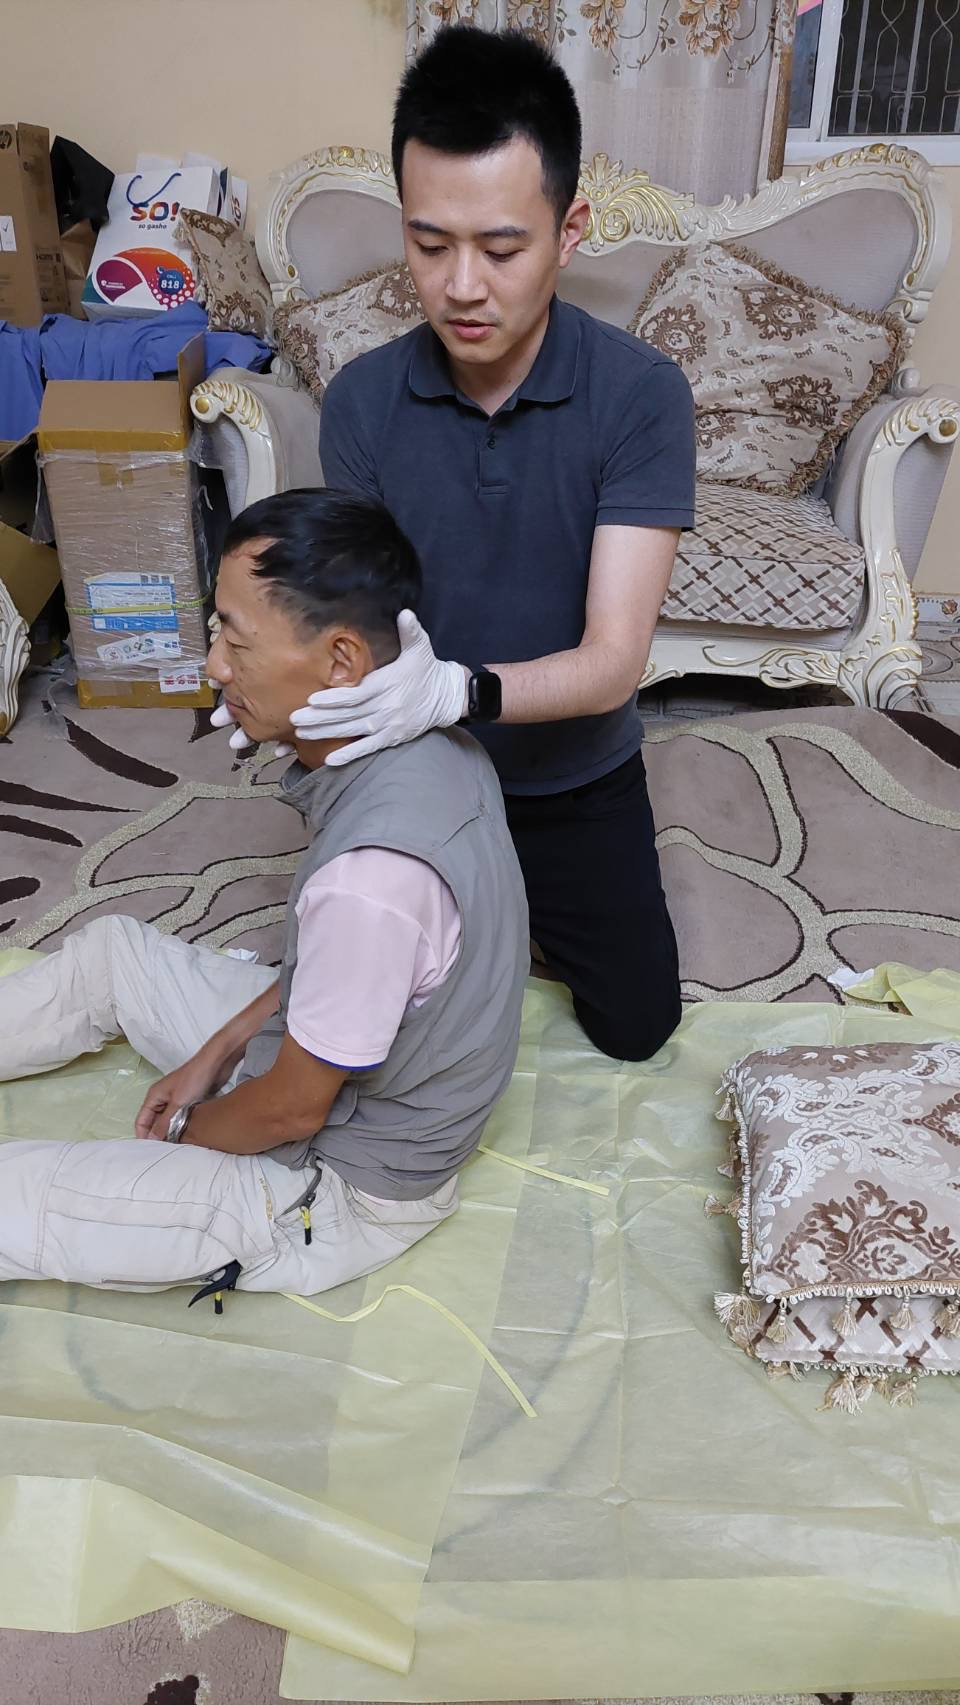
\includegraphics[width=0.20\textwidth]{IMG-2338.JPG}
    \end{center}
\end{frame}

%%%%
\begin{frame}
\frametitle{TMM's Projects - second pillar}
% Add content here
\begin{outline}    
    \1 capacity building for staffs
        %\2 Contributing to system and equipment upgrades in the orthopedic ward
        \2 \textcolor{red}{On-the-job training} for local doctors to improve their skills and care, in the departments of internal medicine, anesthesiology, orthopedic, obstetricy, emergency, intensive care unit, and maxillofacial surgery in HGH.
        \2 Teaching \textcolor{red}{nurses} basic skills in HGH.        
        \2 Instructing interns at \textcolor{red}{the University of Hargeisa (UoH)}.
        
    \1 capacity building for equipments
        \2 In operation theatre (OT), supporting video intubation system, surgical tables, C-arm X-ray, arthroscopic shaver, maxillofacial/orthopedic instruments/implants, and other \textcolor{red}{medical devices and medicines} for use in HGH.

        \2 Building trauma kits for Somaliland \textcolor{red}{army force}.
        %\2 Assist in establishing department of urology in HGH and their resident training program

\end{outline}
\end{frame}

\begin{frame}{Capacity building: orthopedic}
    \begin{center}i
        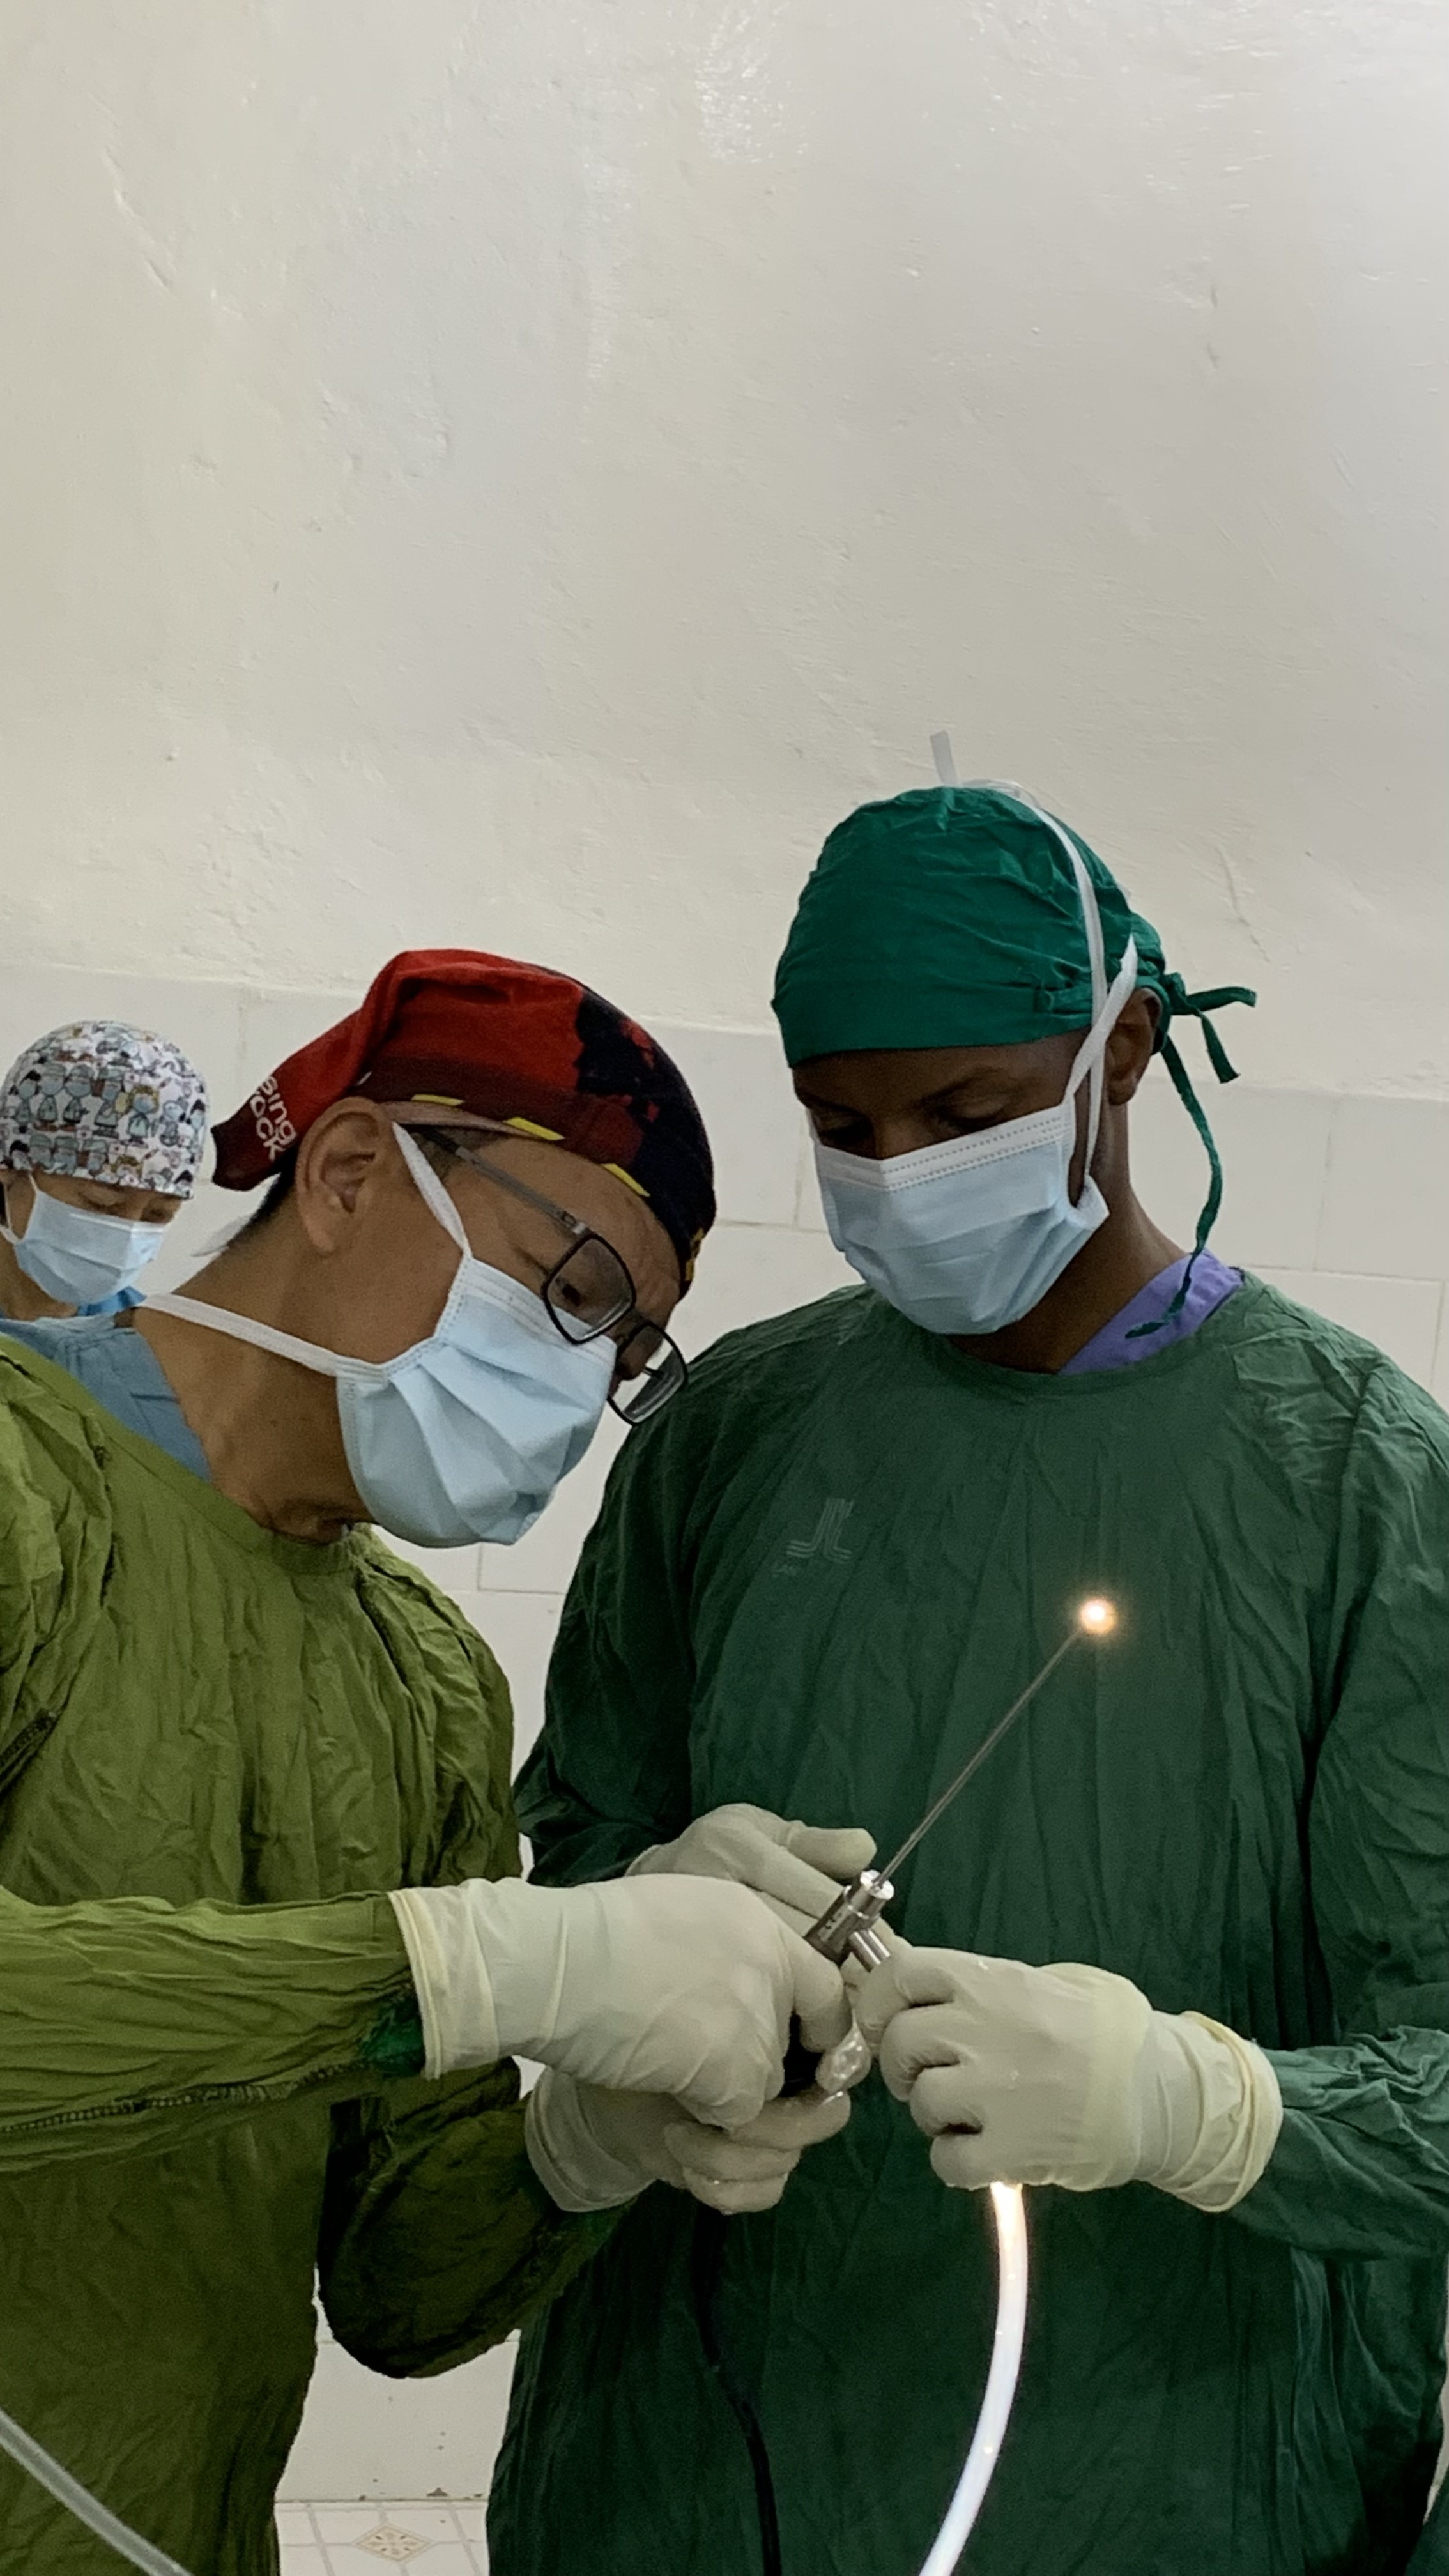
\includegraphics[width=0.30\textwidth]{IMG-6067.jpg}
        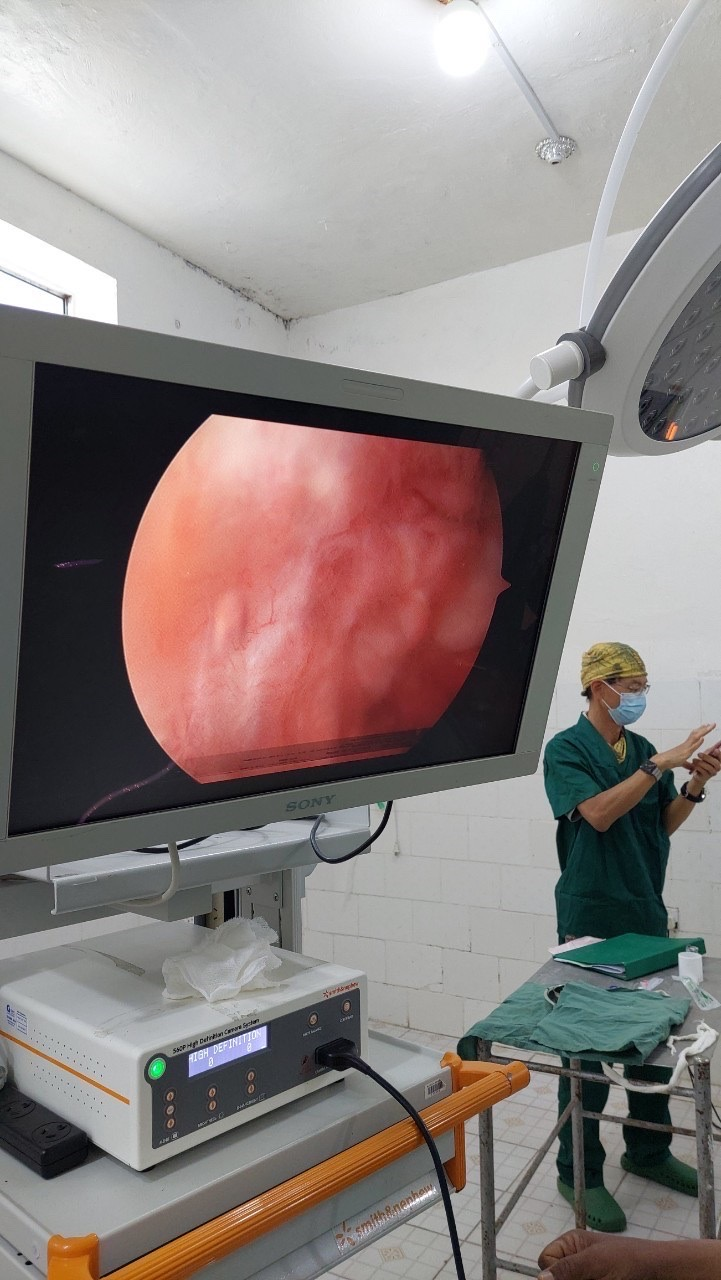
\includegraphics[width=0.30\textwidth]{IMG-6227.JPG}
    \end{center}
\end{frame}


\begin{frame}{Capacity building: nurse, urology}
    \begin{center}
        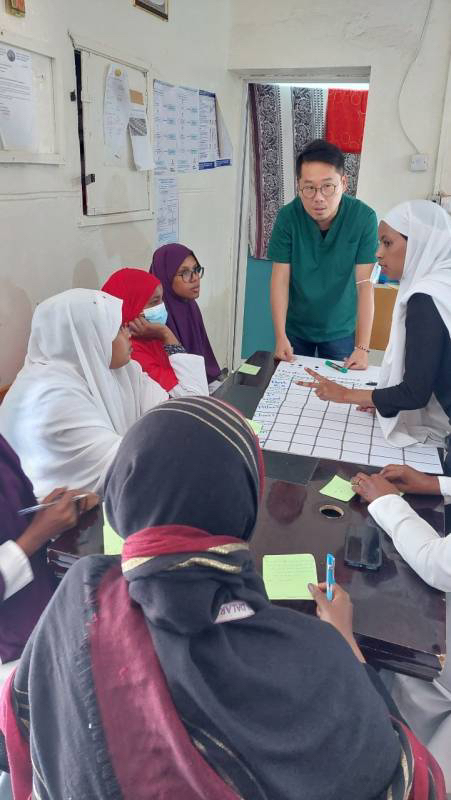
\includegraphics[width=0.30\textwidth]{6963.jpg}
        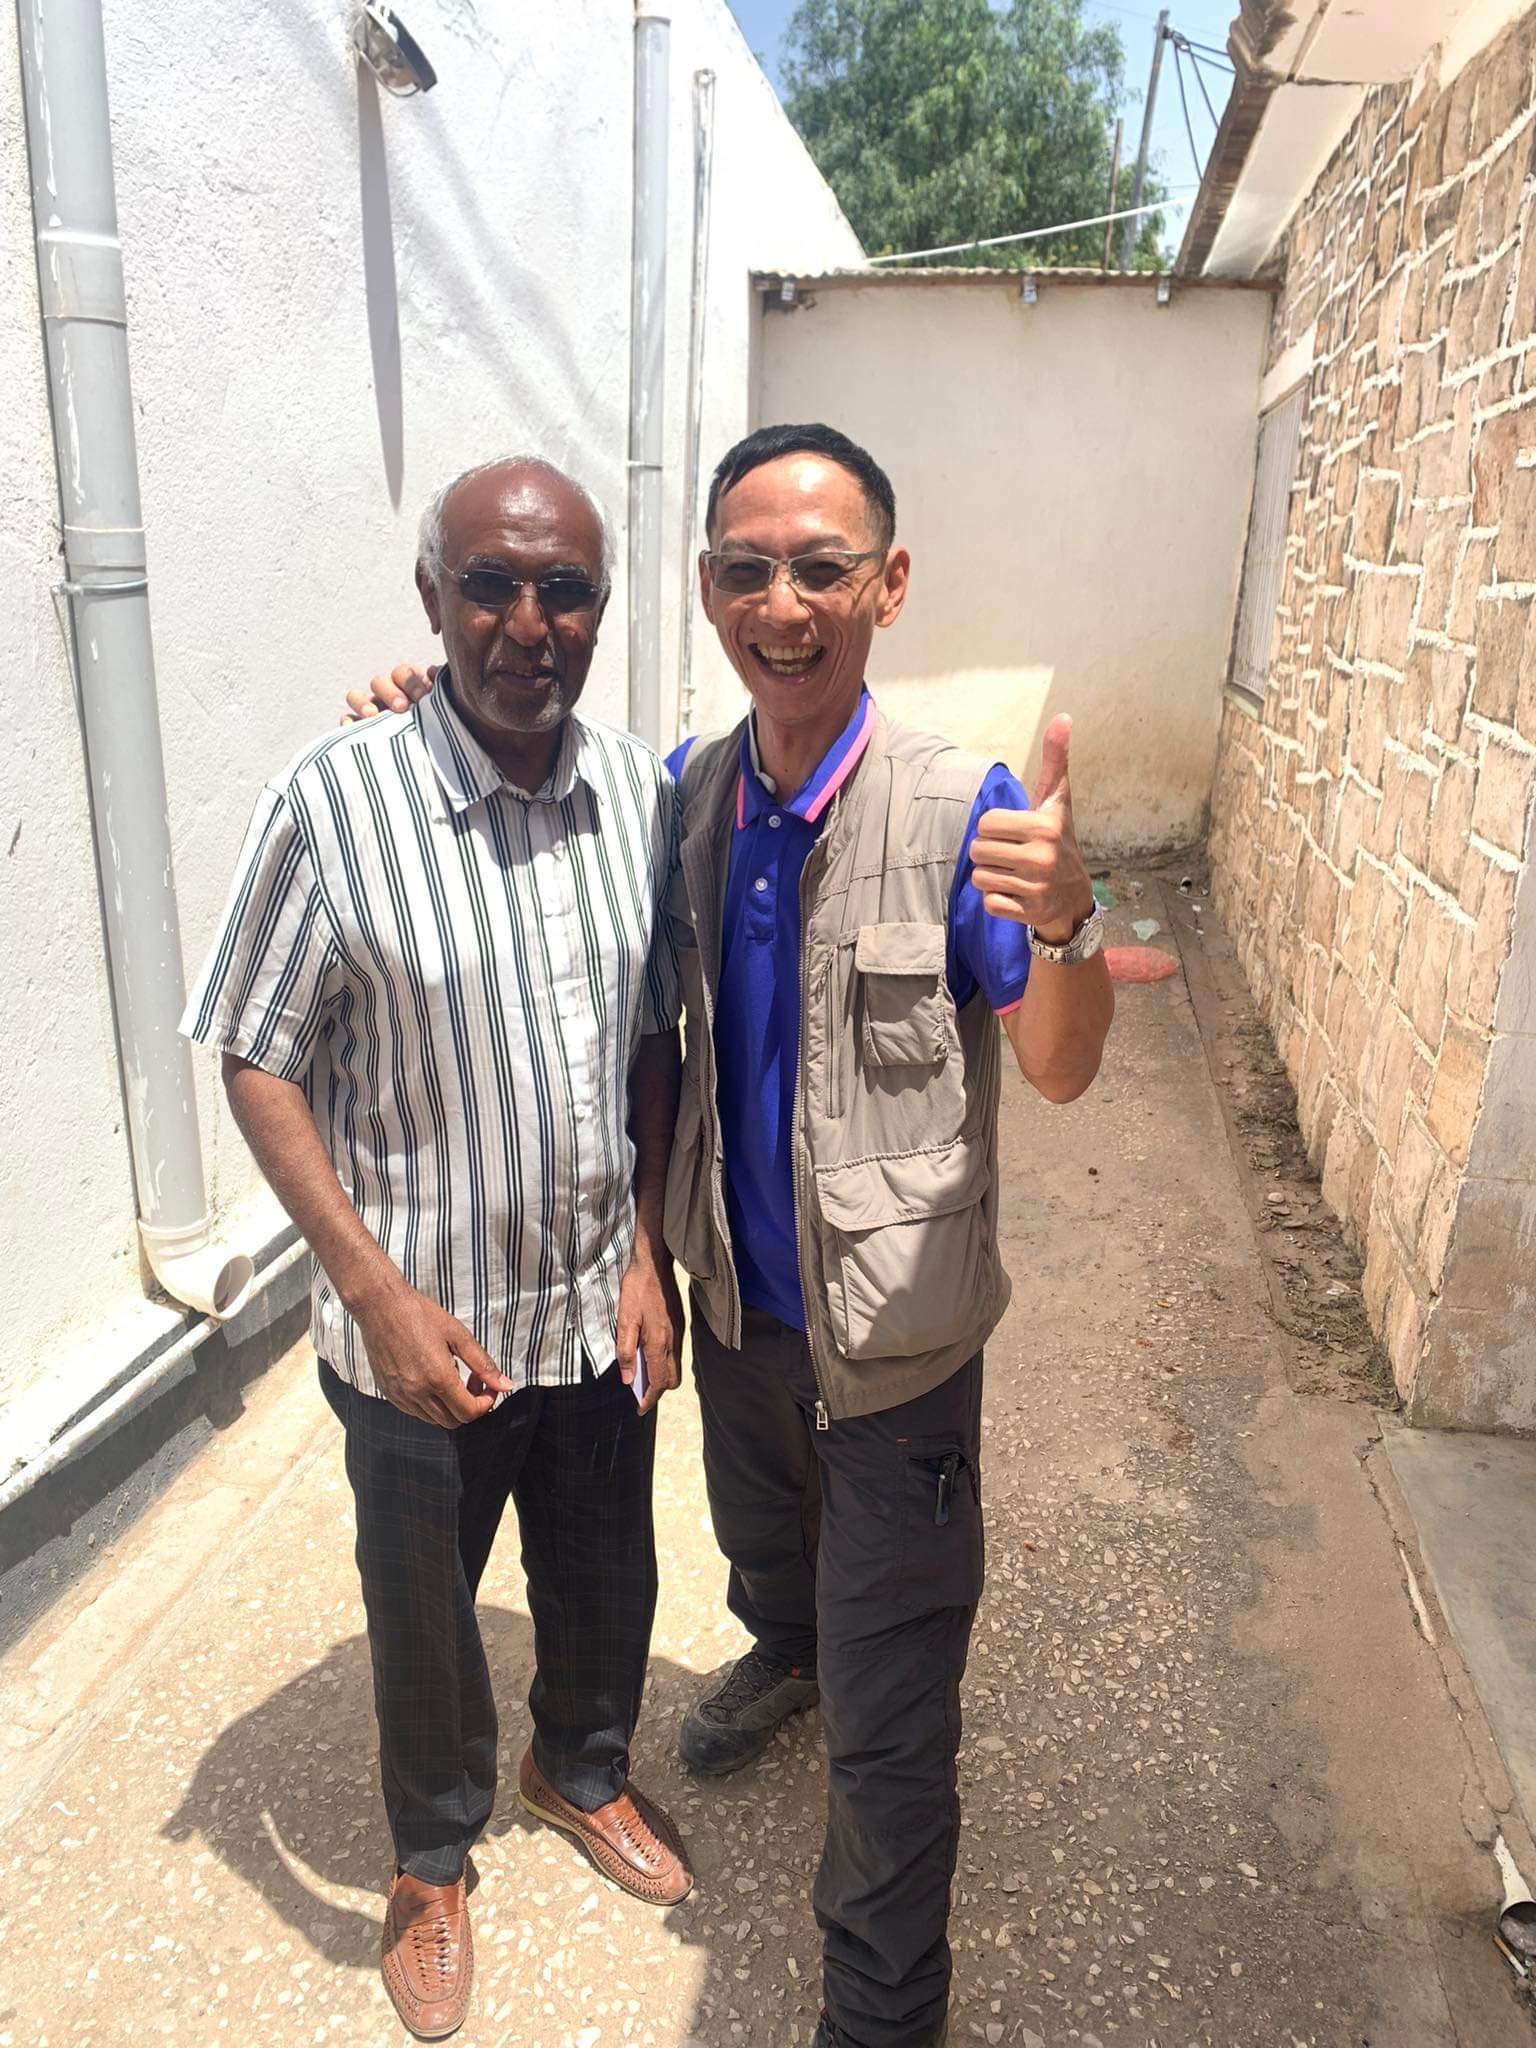
\includegraphics[width=0.30\textwidth]{IMG_5040.jpeg}
    \end{center}
\end{frame}



\begin{frame}{Capacity building: trauma kits supplies}
    \begin{center}
        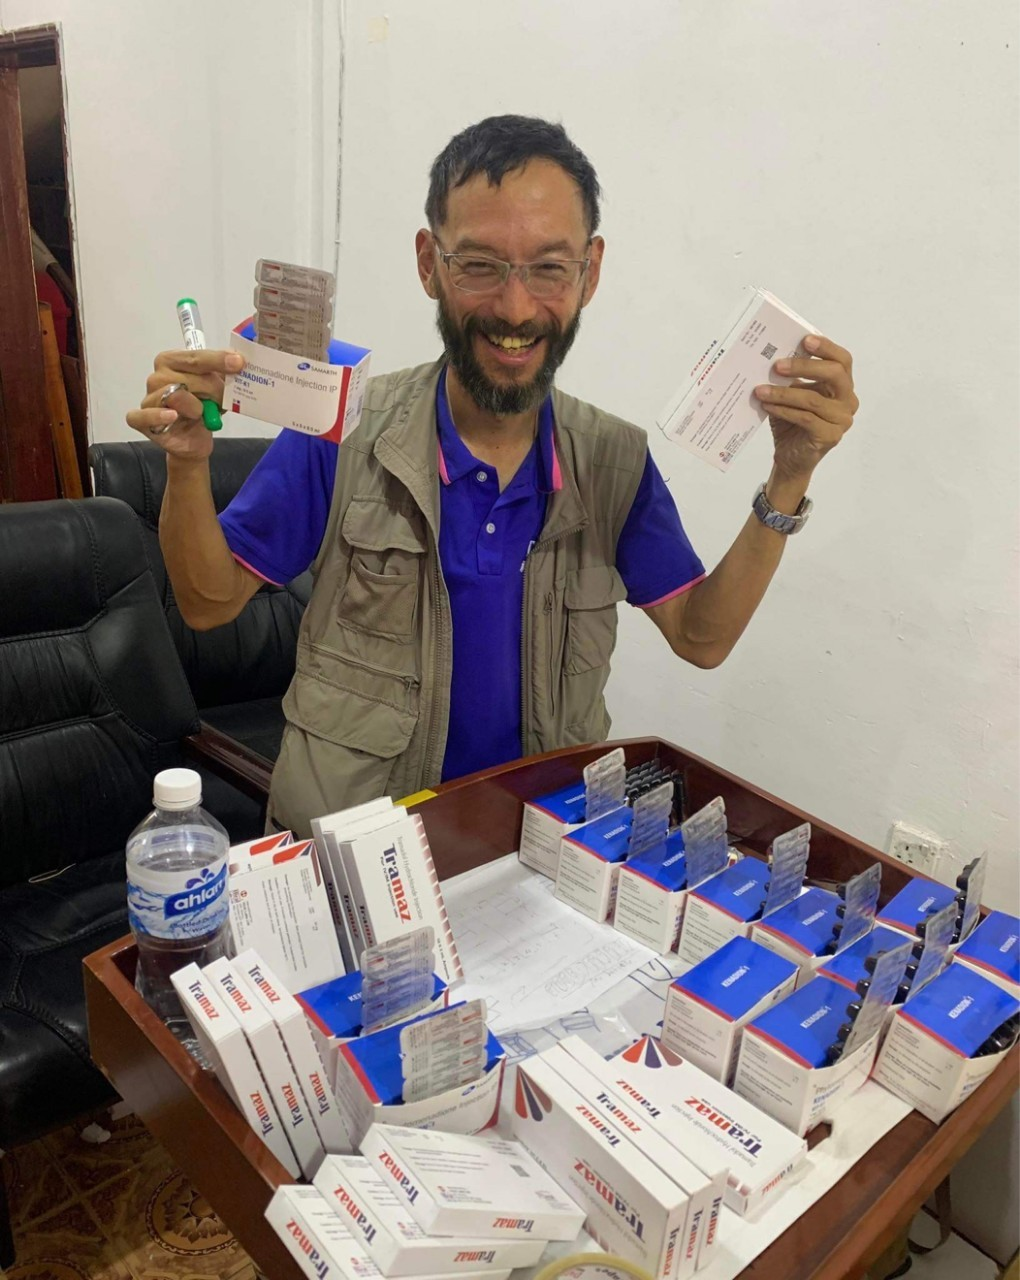
\includegraphics[width=0.33\textwidth]{4875890938550512937.32a296a9eebb4034c36c698f4a25d9d0.23050612.JPG}
        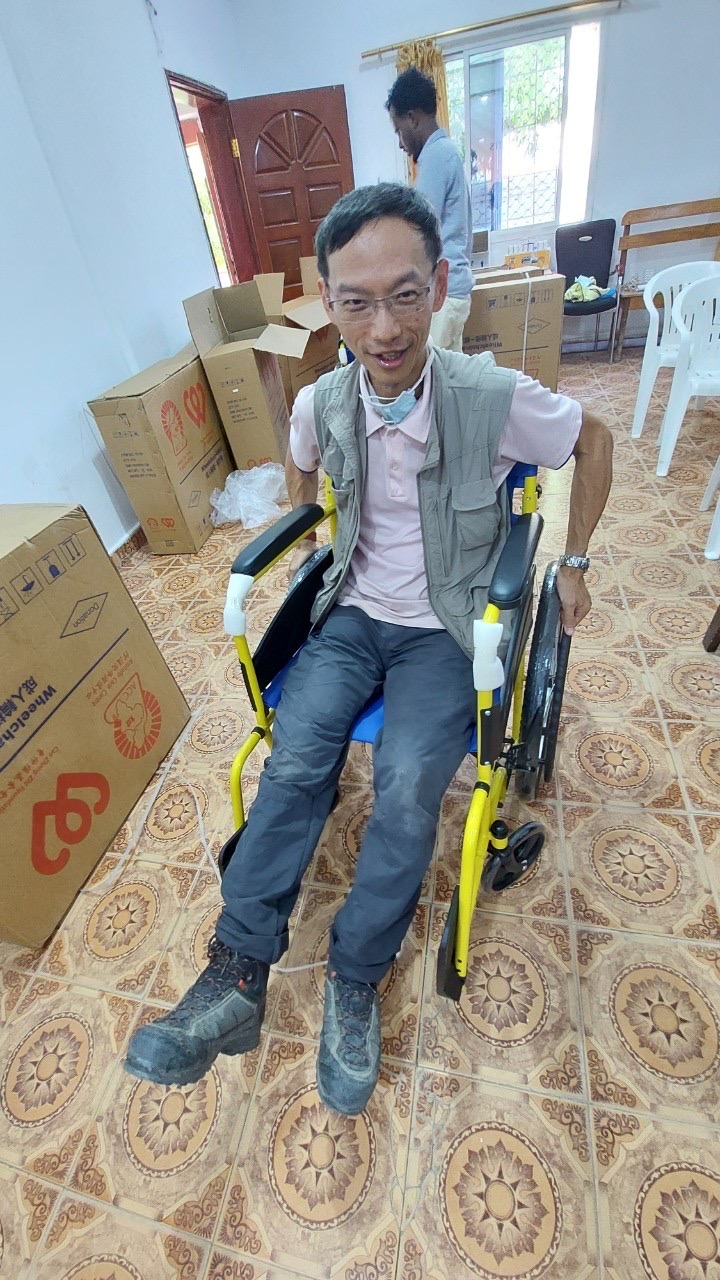
\includegraphics[width=0.30\textwidth]{IMG-2655.JPG}
        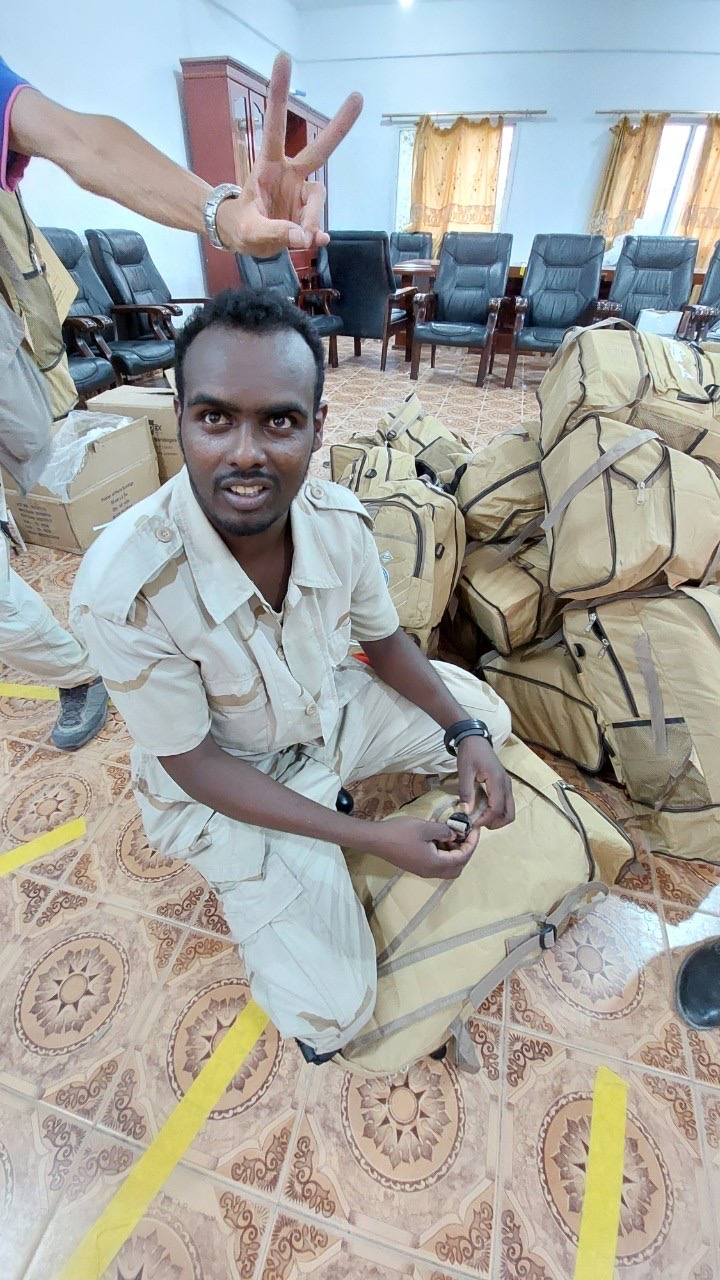
\includegraphics[width=0.30\textwidth]{IMG-2313.JPG}
%        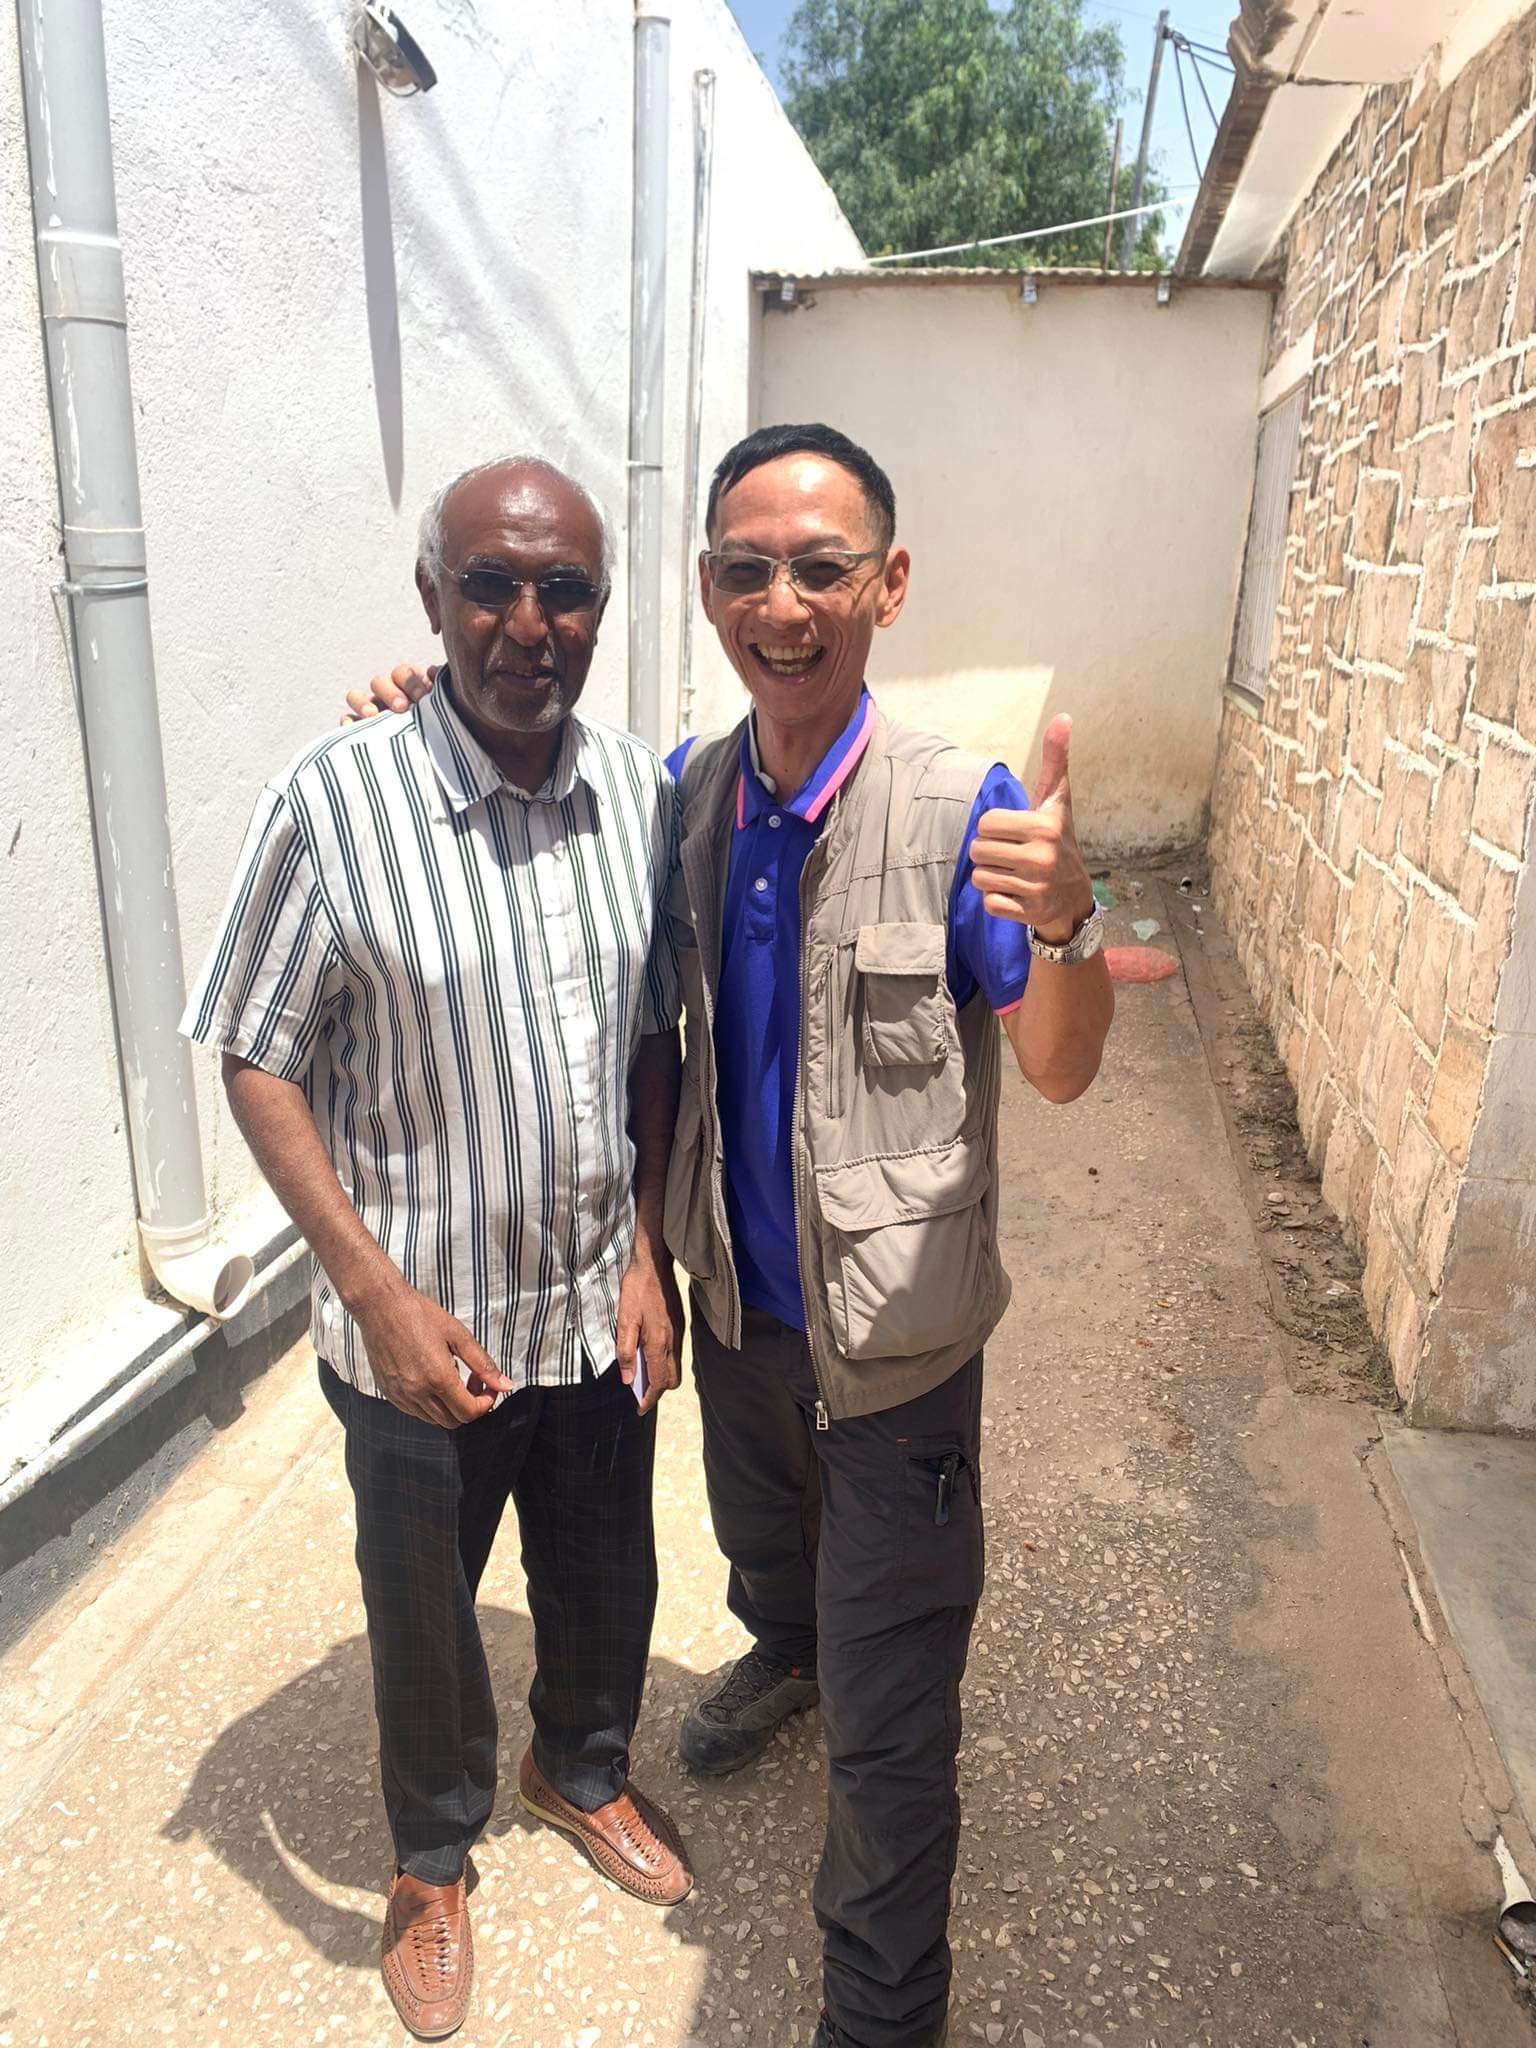
\includegraphics[width=0.24\textwidth]{IMG_5040.jpeg}    
    \end{center}
\end{frame}

\begin{frame}{Capacity building: trauma kits supplies}
    \begin{center}
        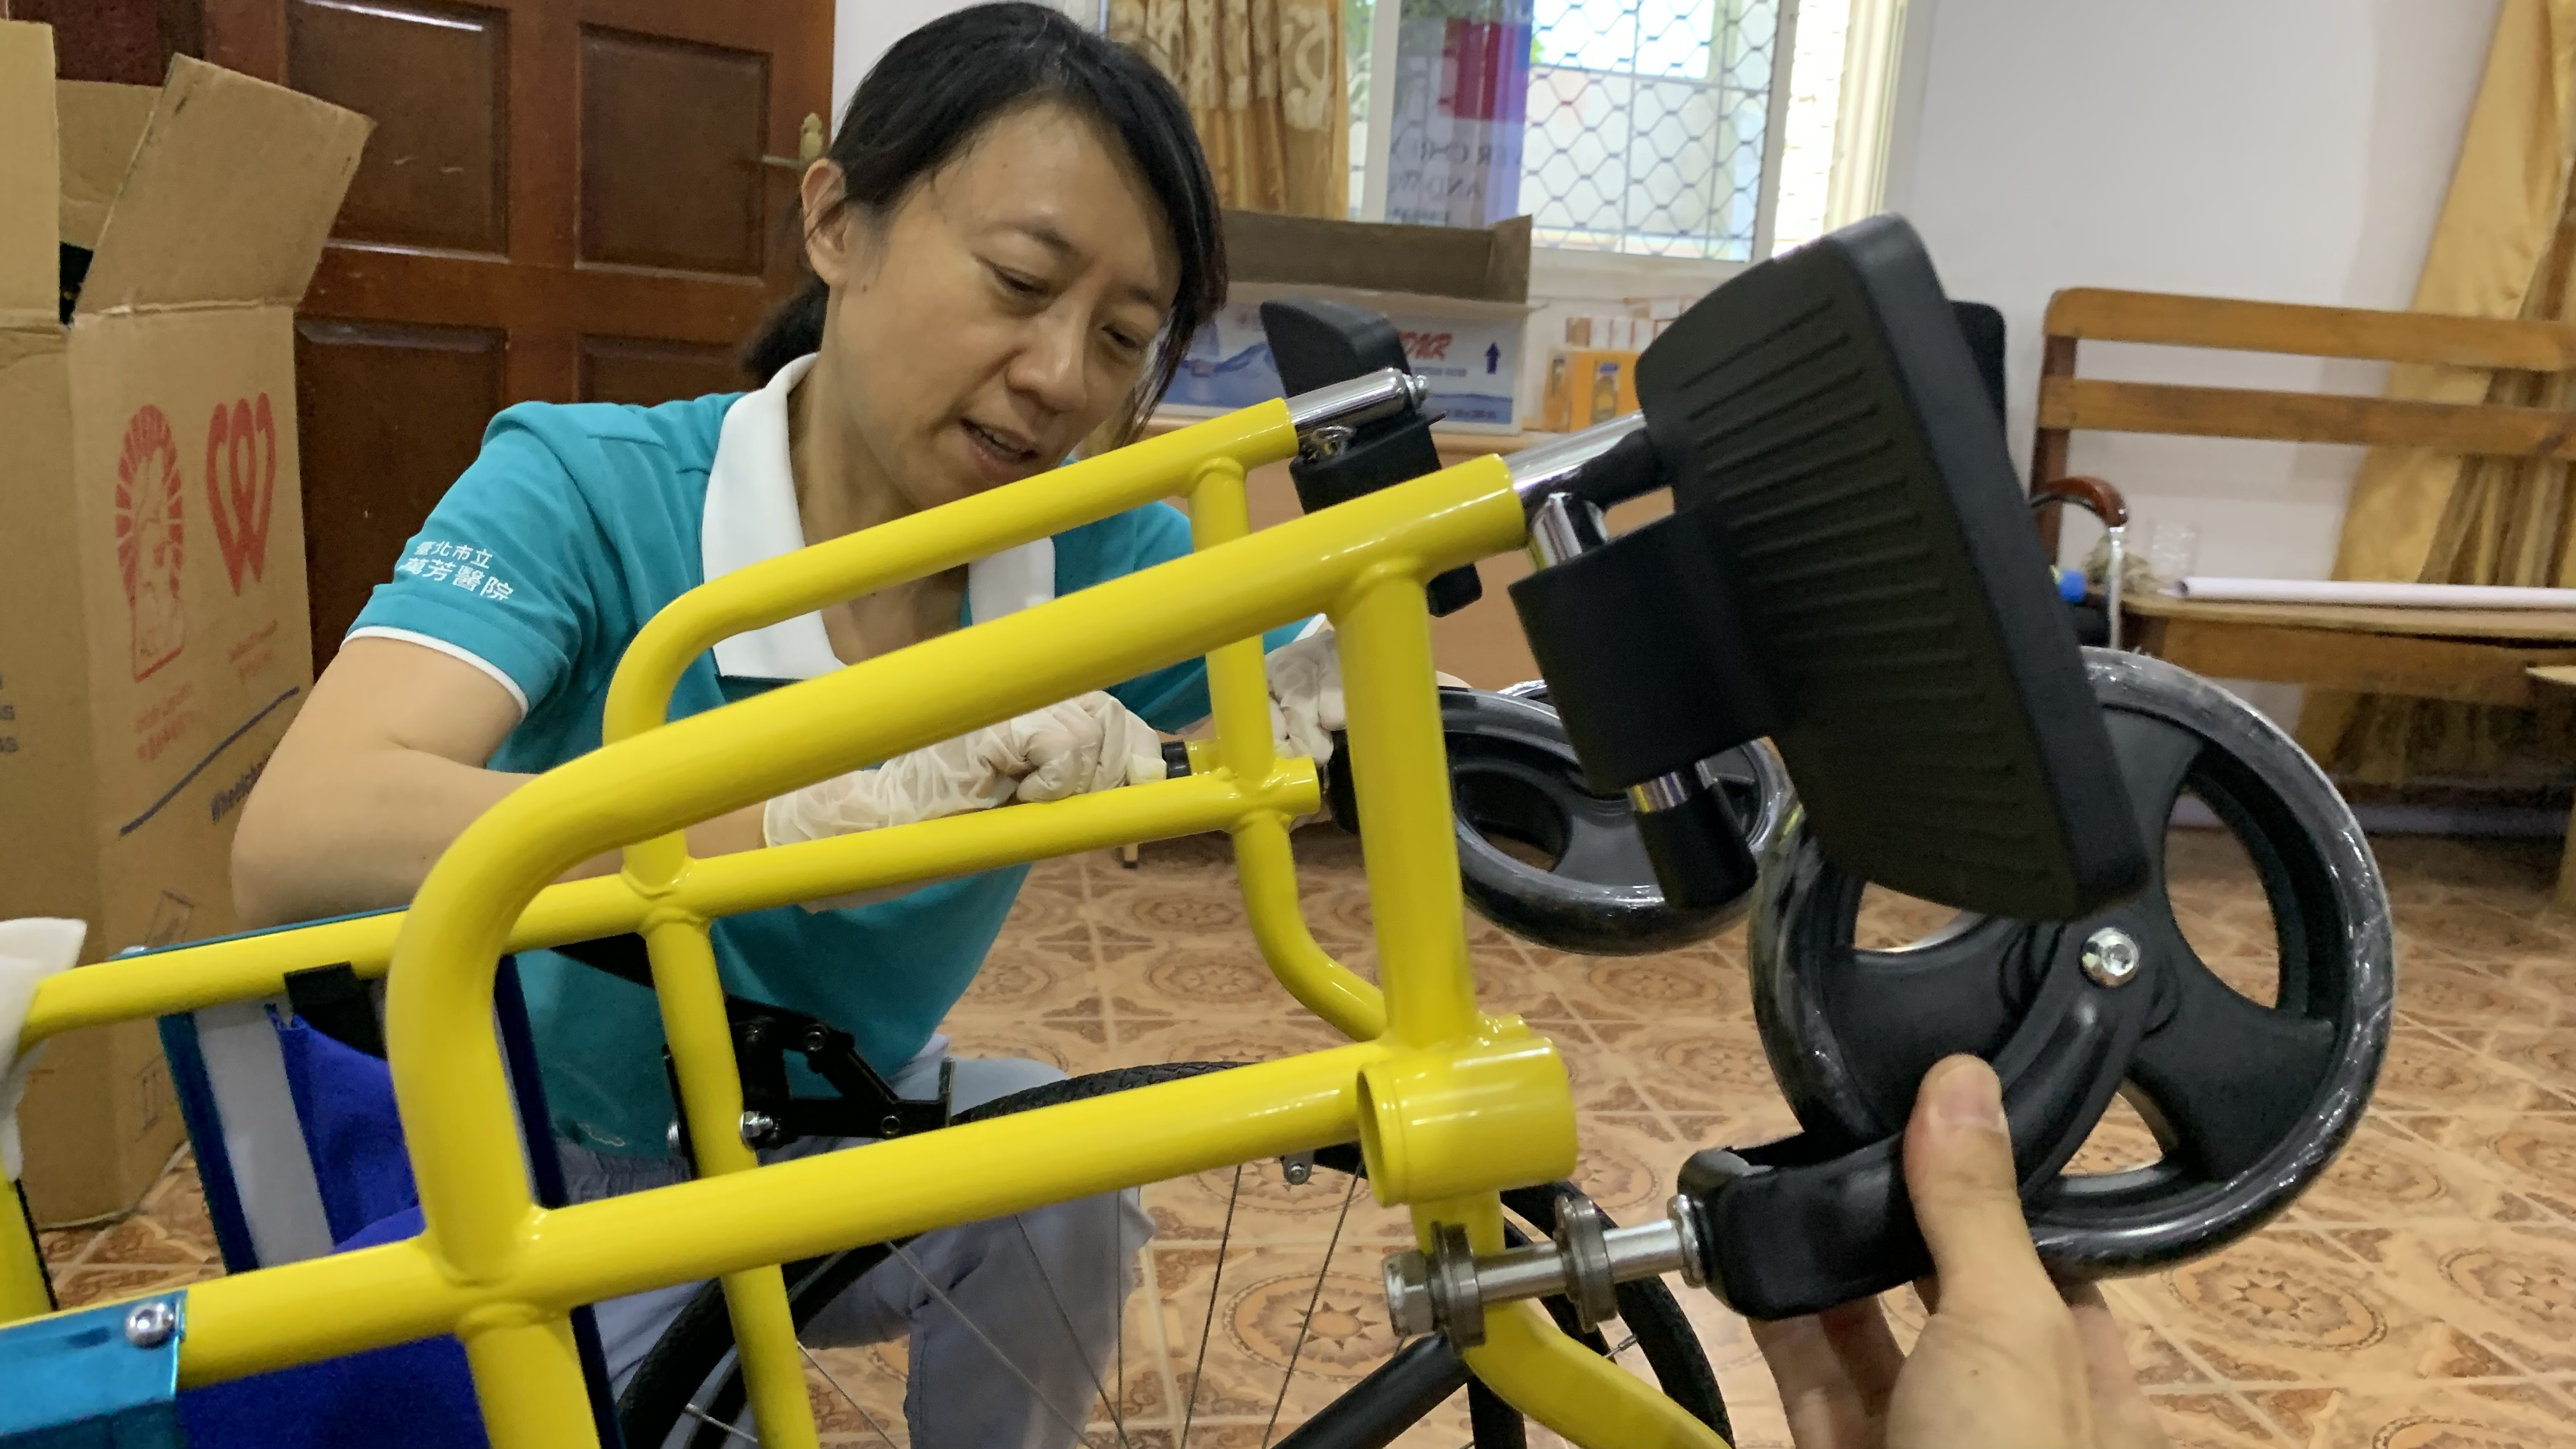
\includegraphics[width=0.4\textwidth]{IMG-2641.jpg}
        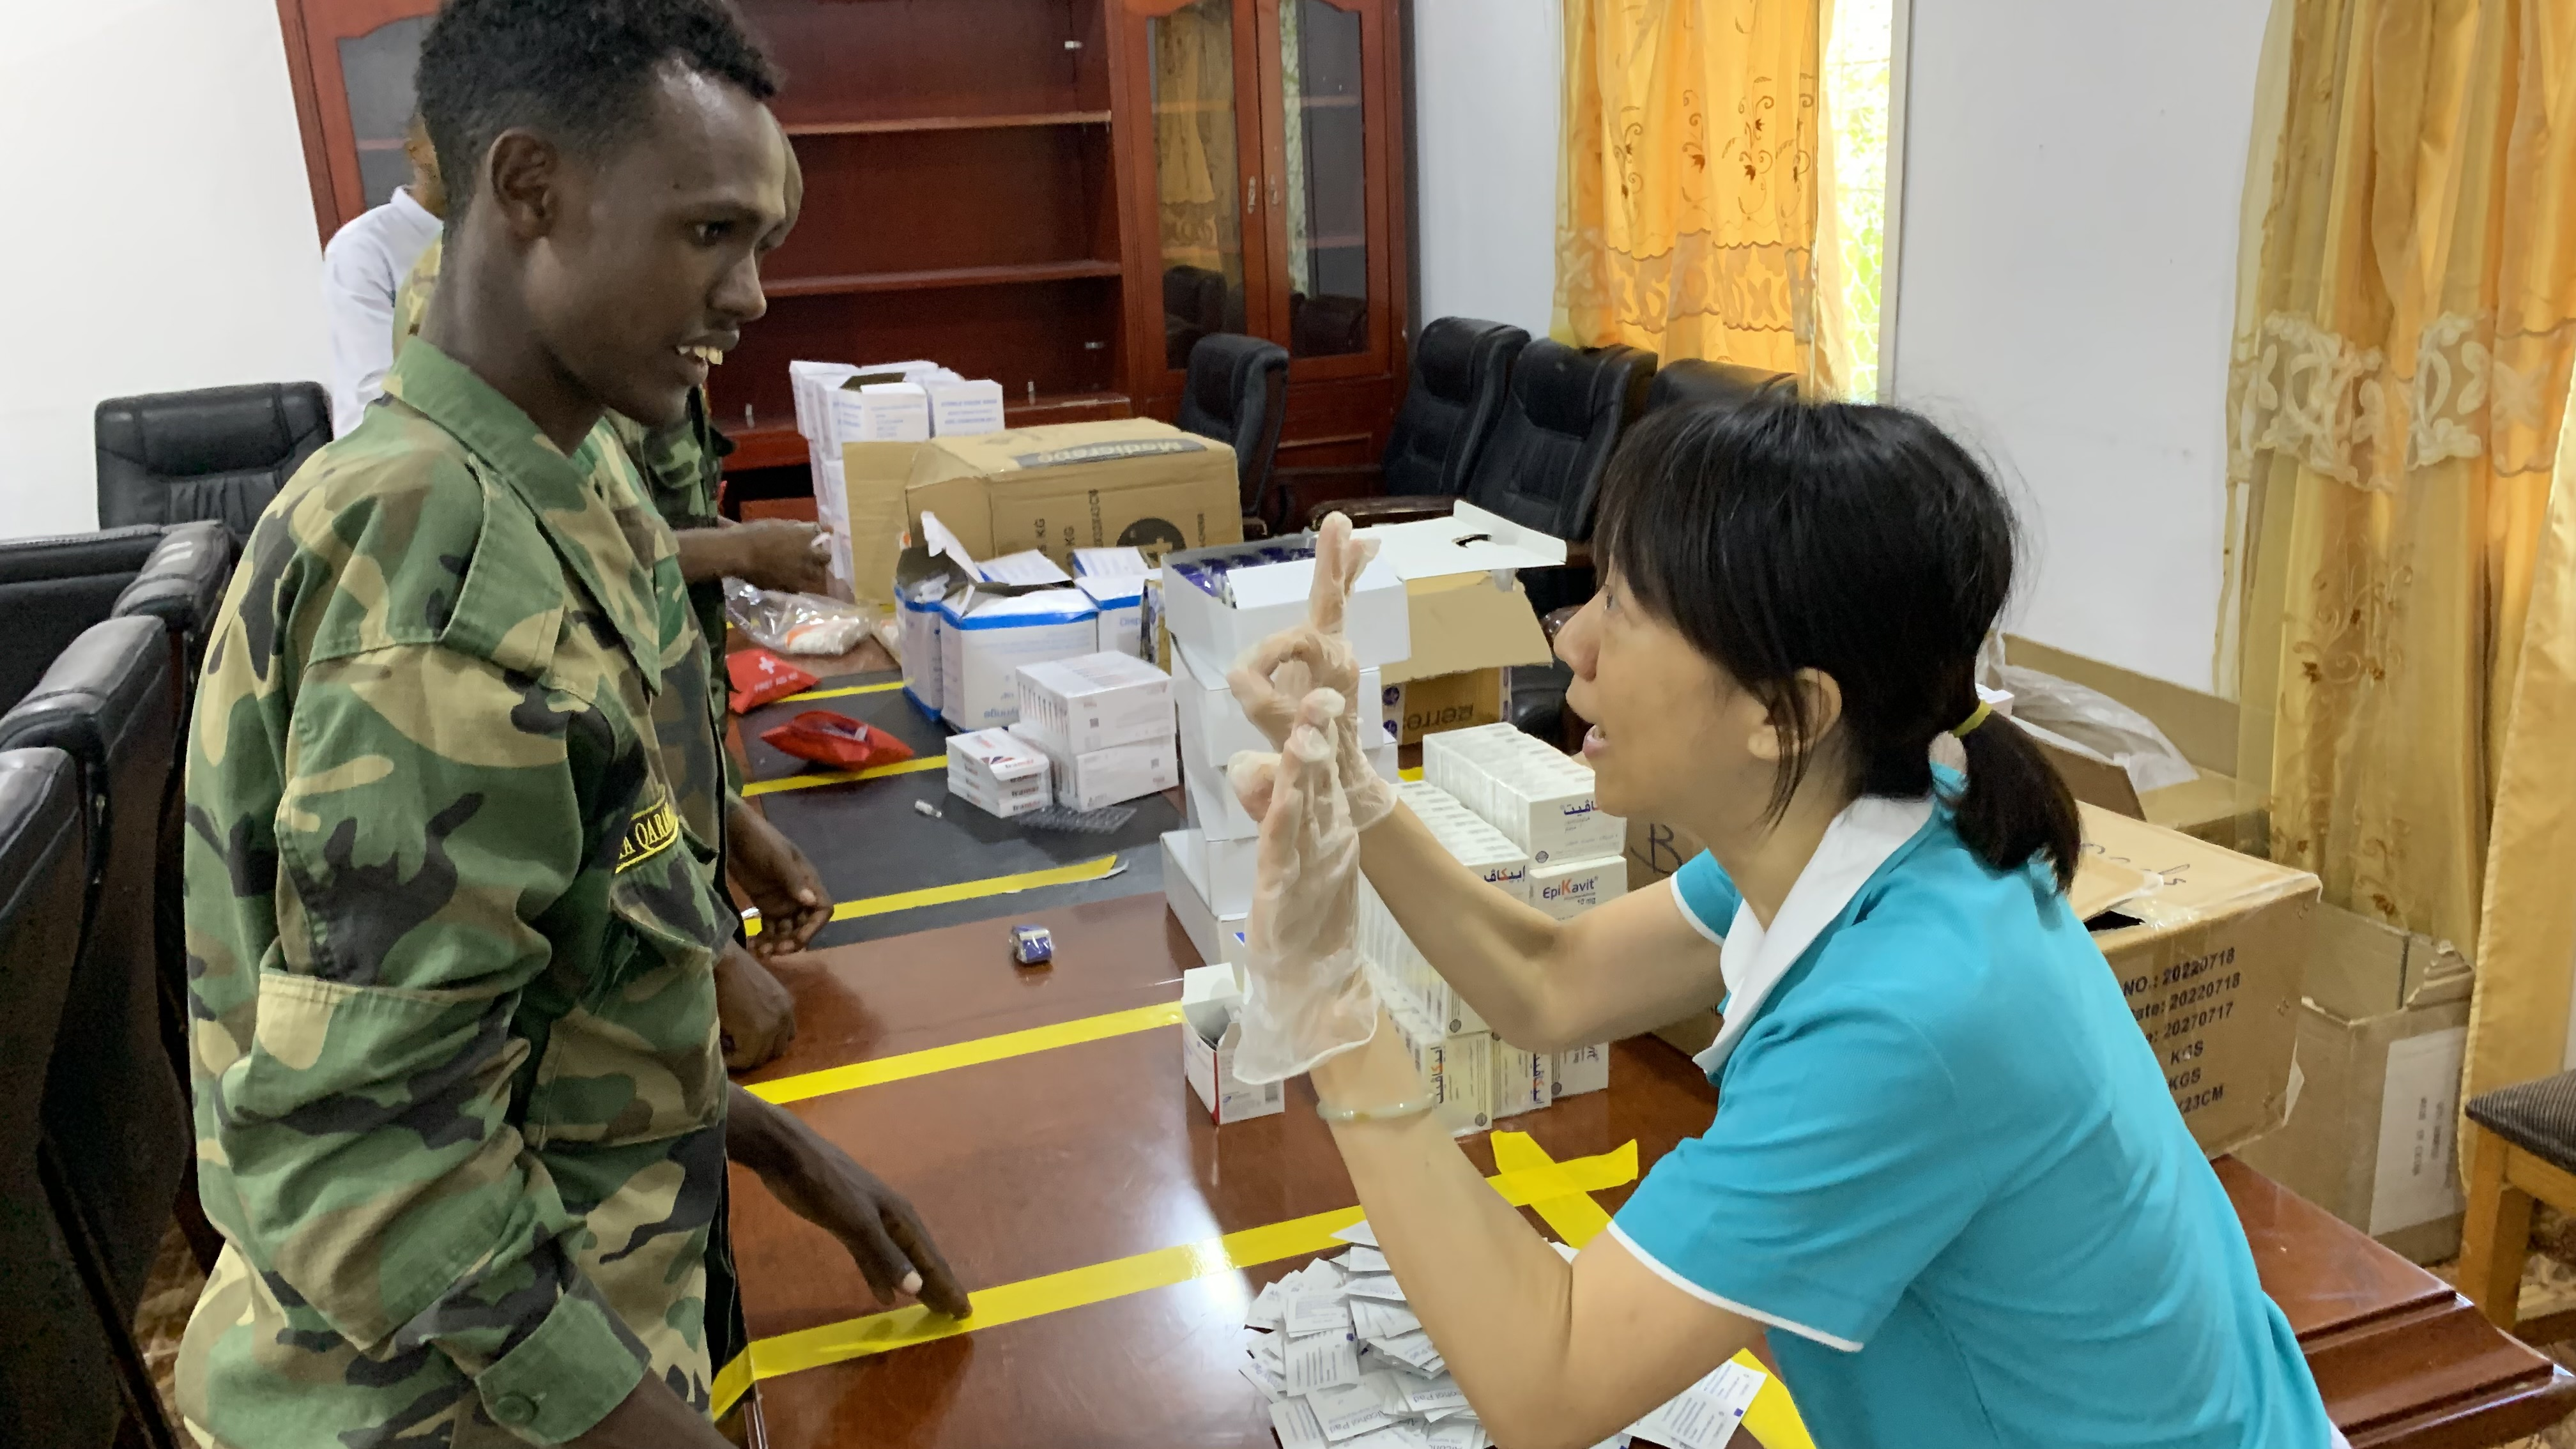
\includegraphics[width=0.4\textwidth]{IMG-2230.jpg} \\
        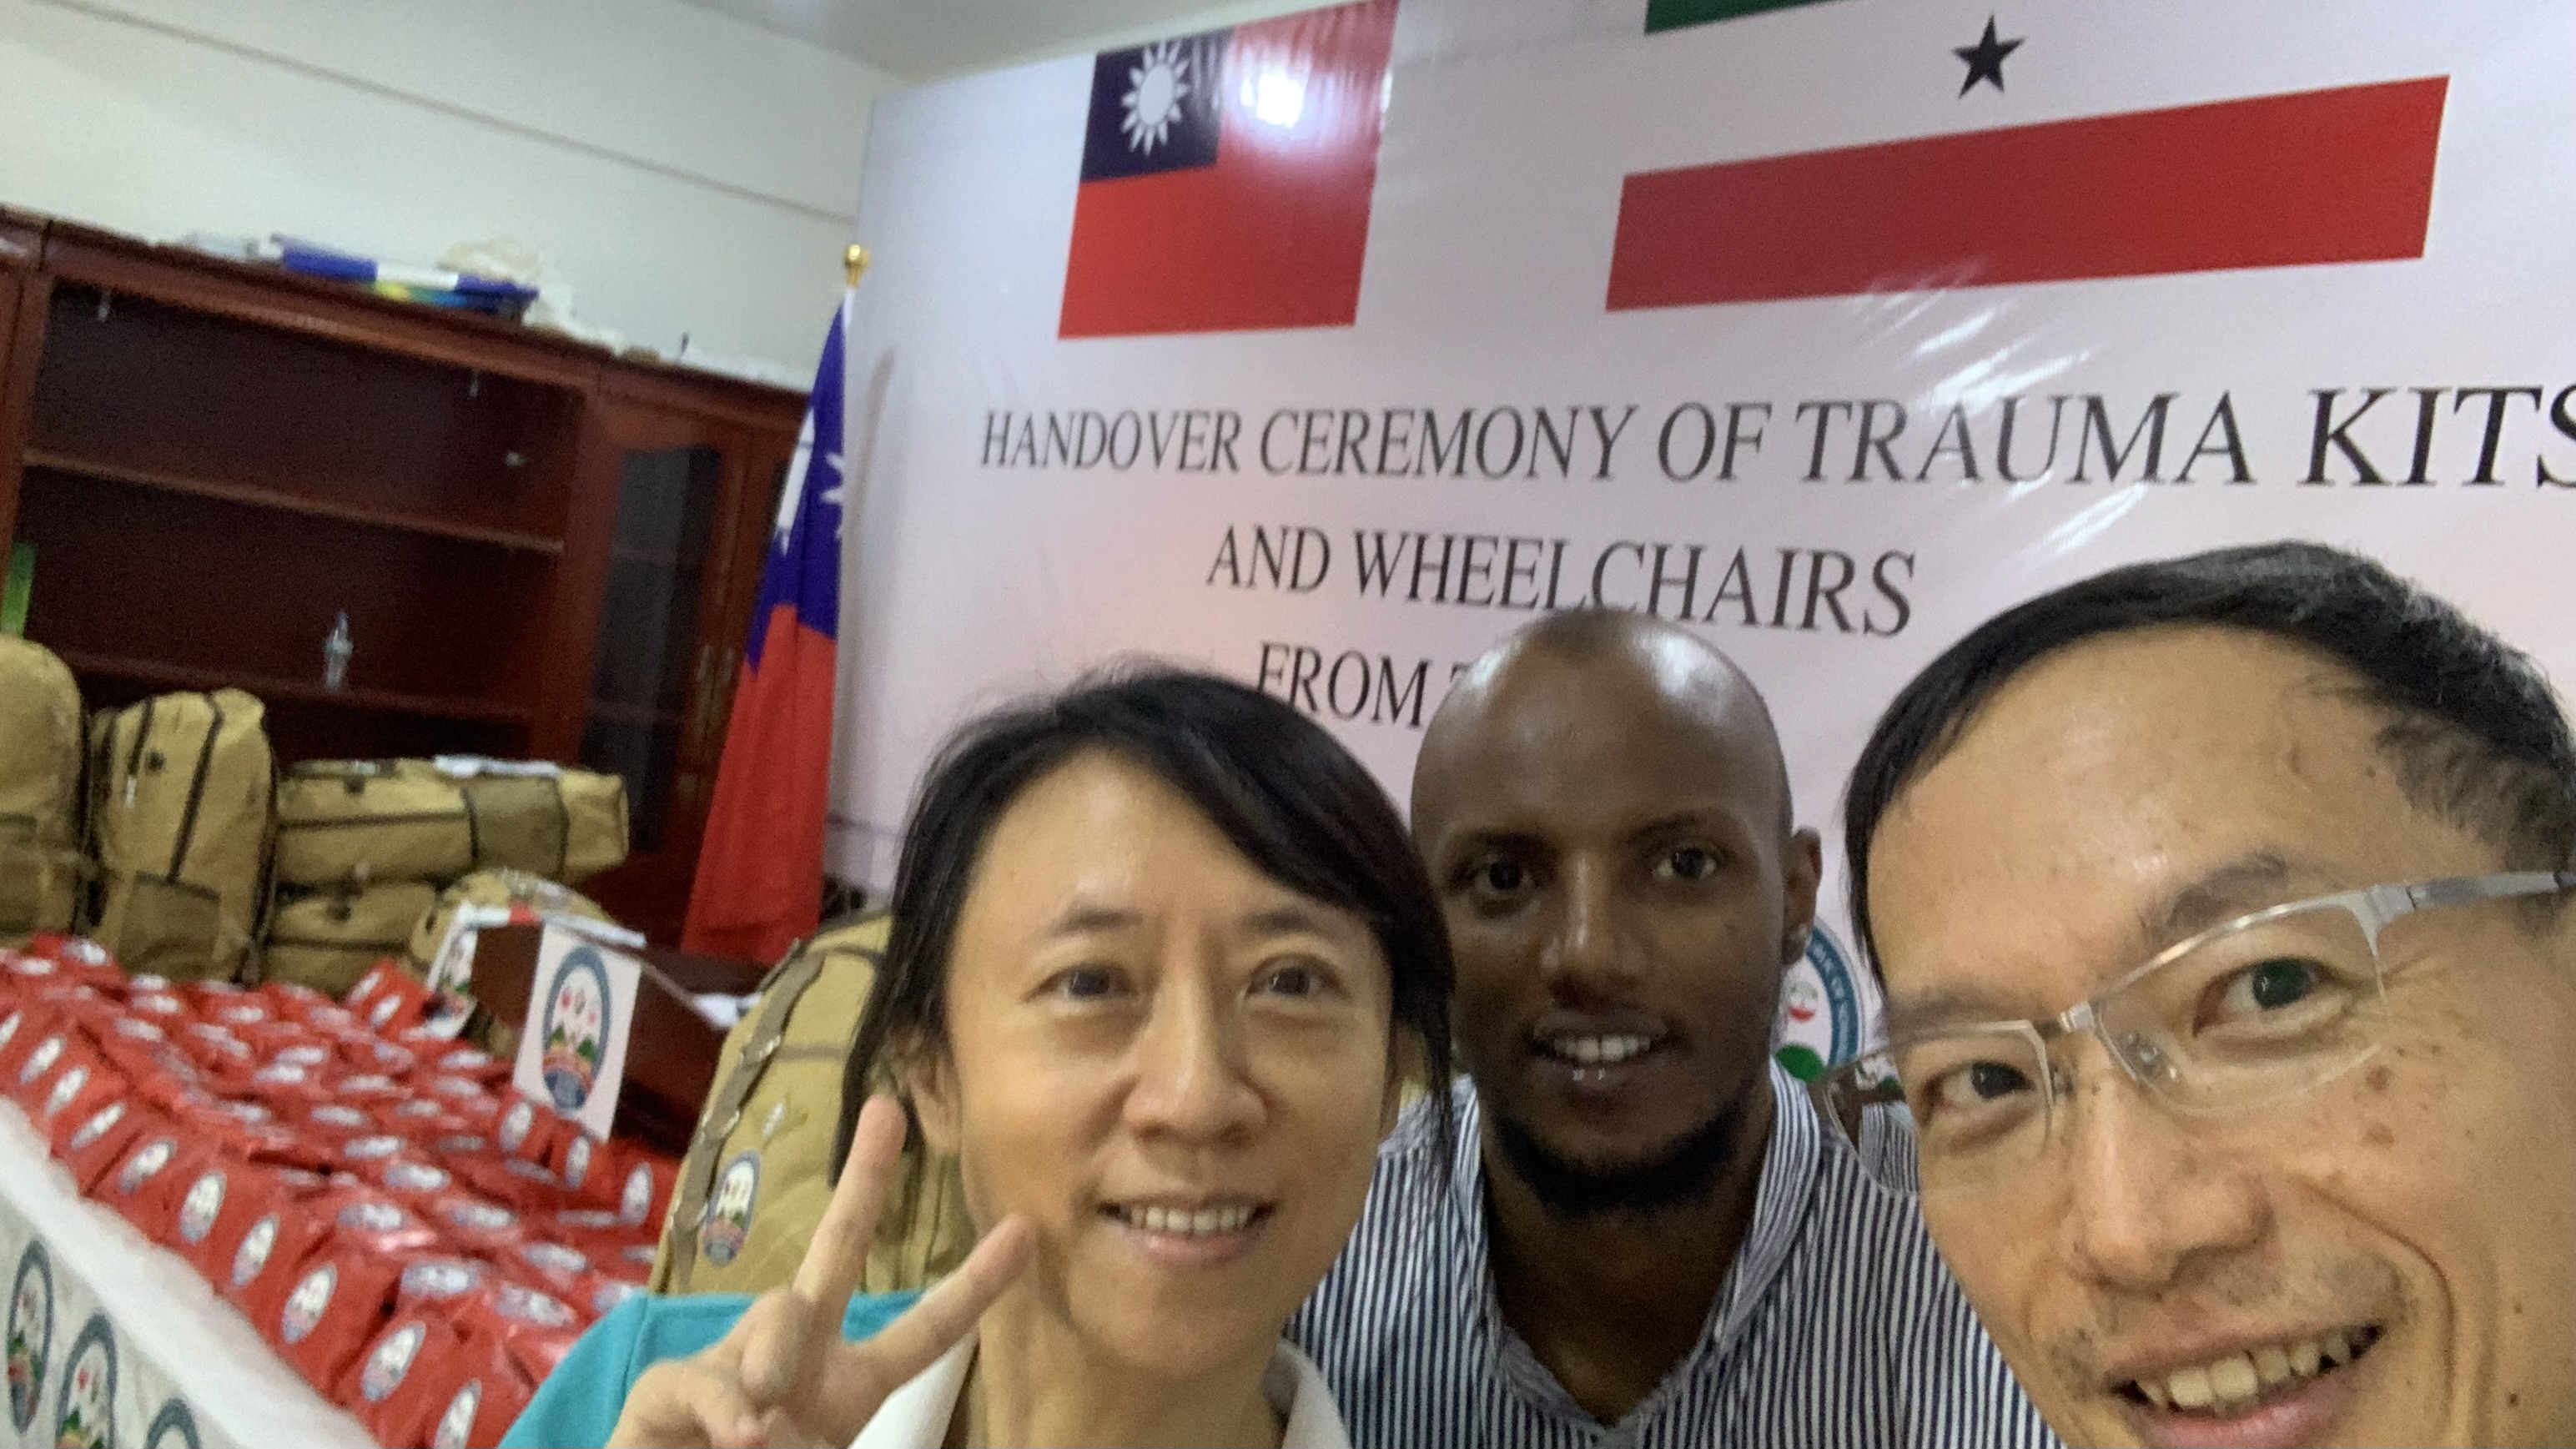
\includegraphics[width=0.4\textwidth]{IMG-2611.jpg}
        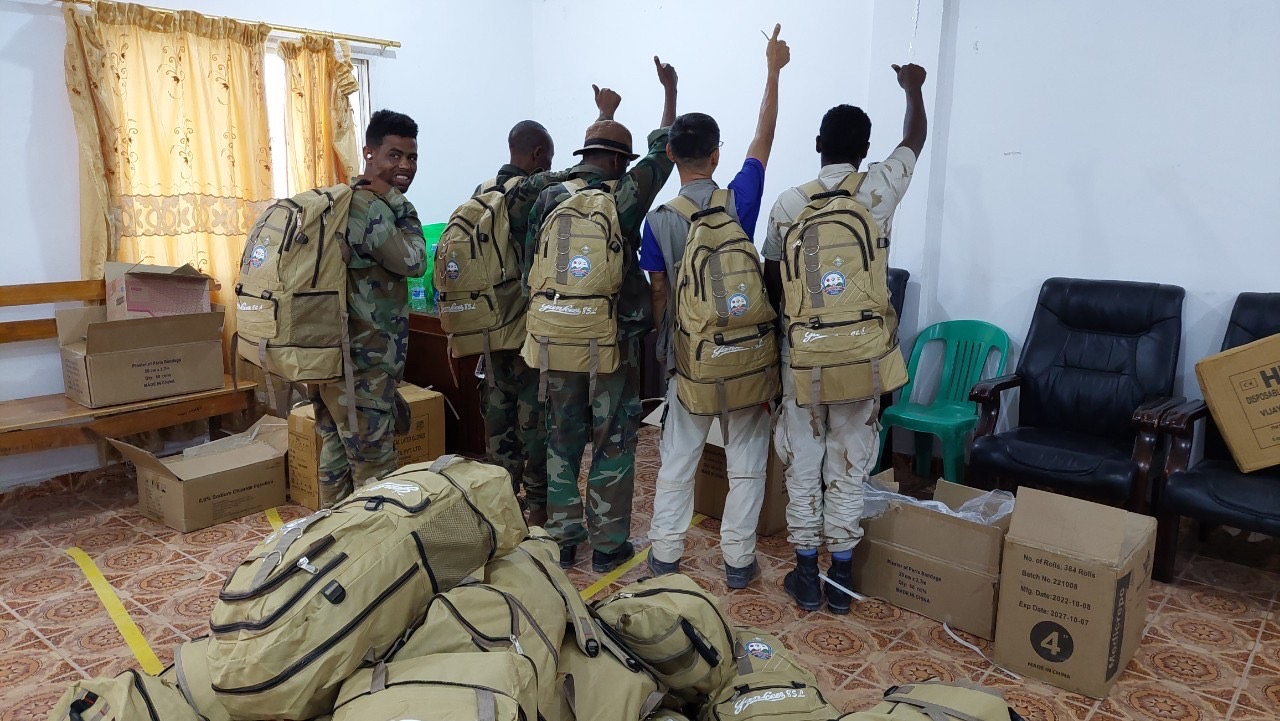
\includegraphics[width=0.4\textwidth]{IMG-2318.JPG}    
    \end{center}
\end{frame}

%%
\begin{frame}{Capacity building: trauma kits supplies}
    \begin{center}
        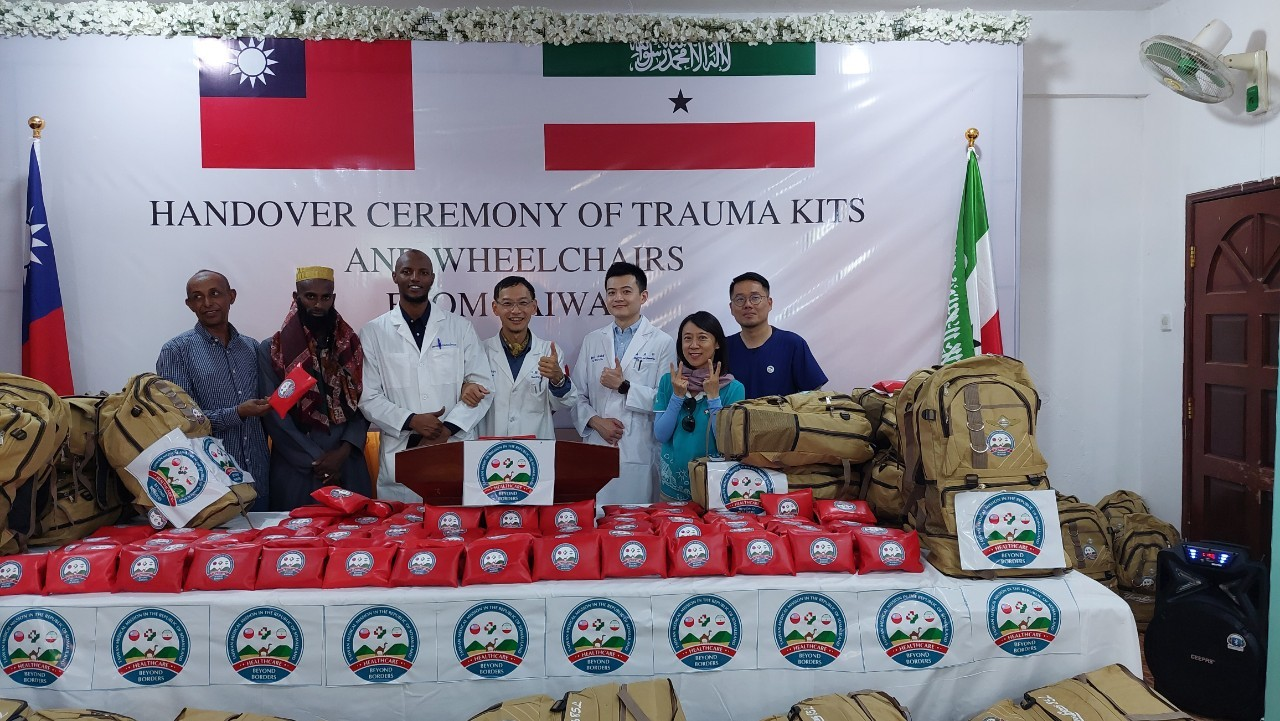
\includegraphics[width=0.8\textwidth]{4879921870343011711.12ba1a84484c21cdb54161b56f33e999.23050712.JPG}
    \end{center}
\end{frame}

\begin{frame}{Capacity building: others}
    \begin{center}
        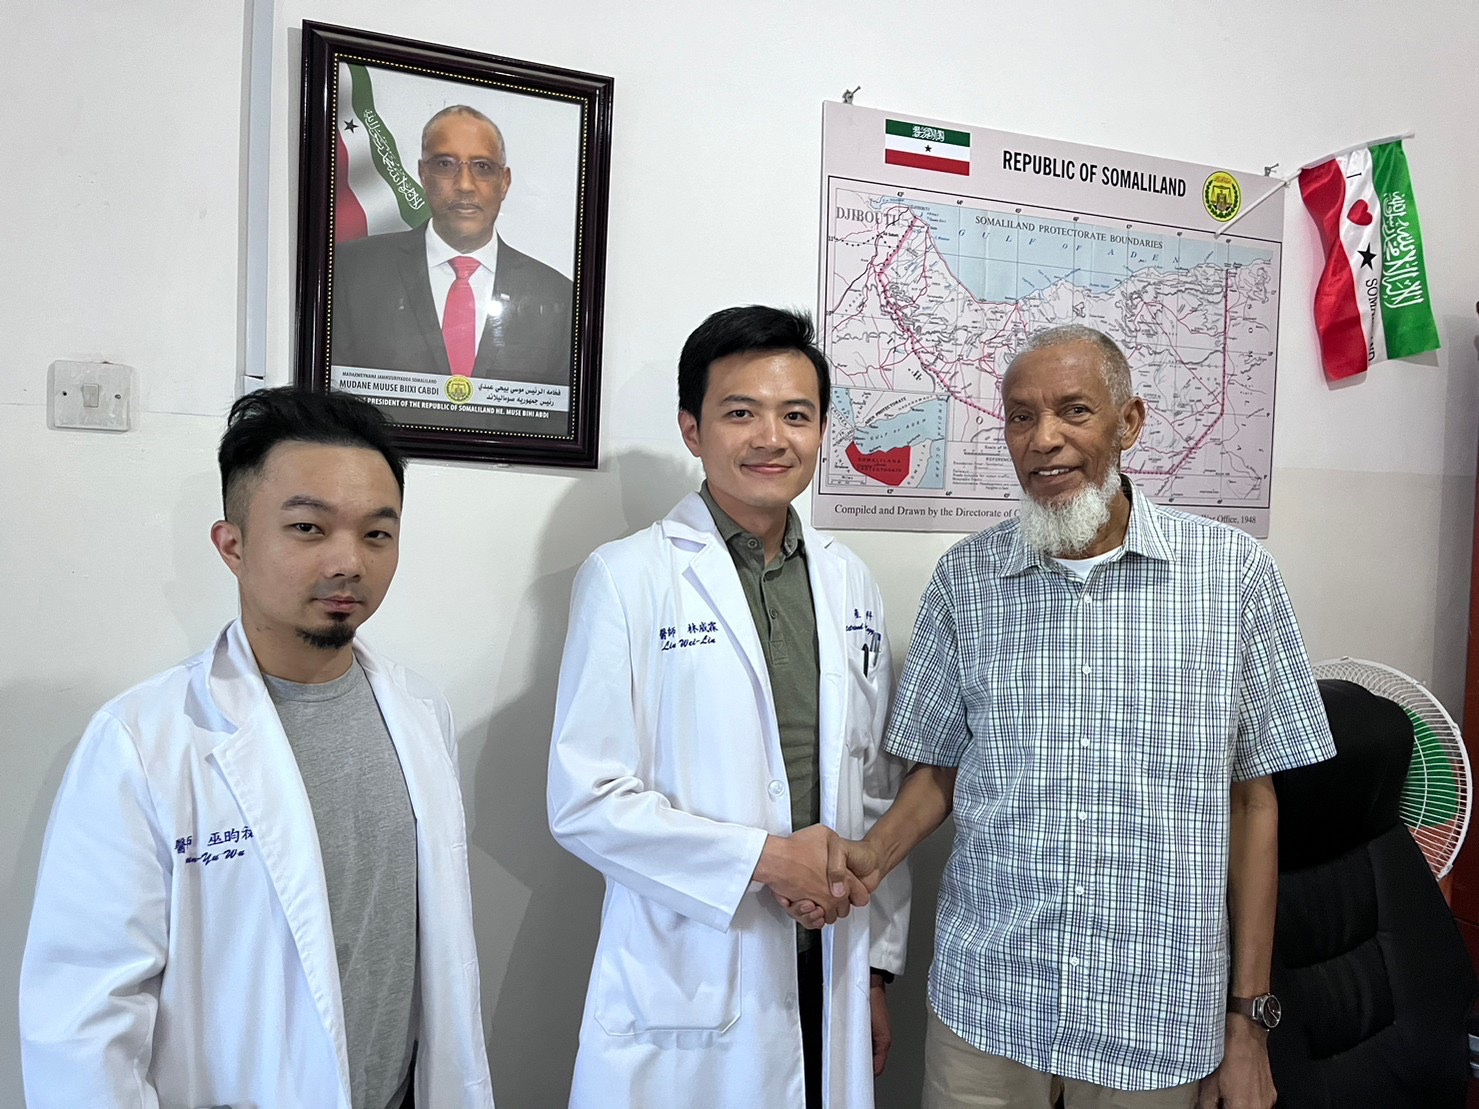
\includegraphics[width=0.24\textwidth]{IMG-5107.JPG}
        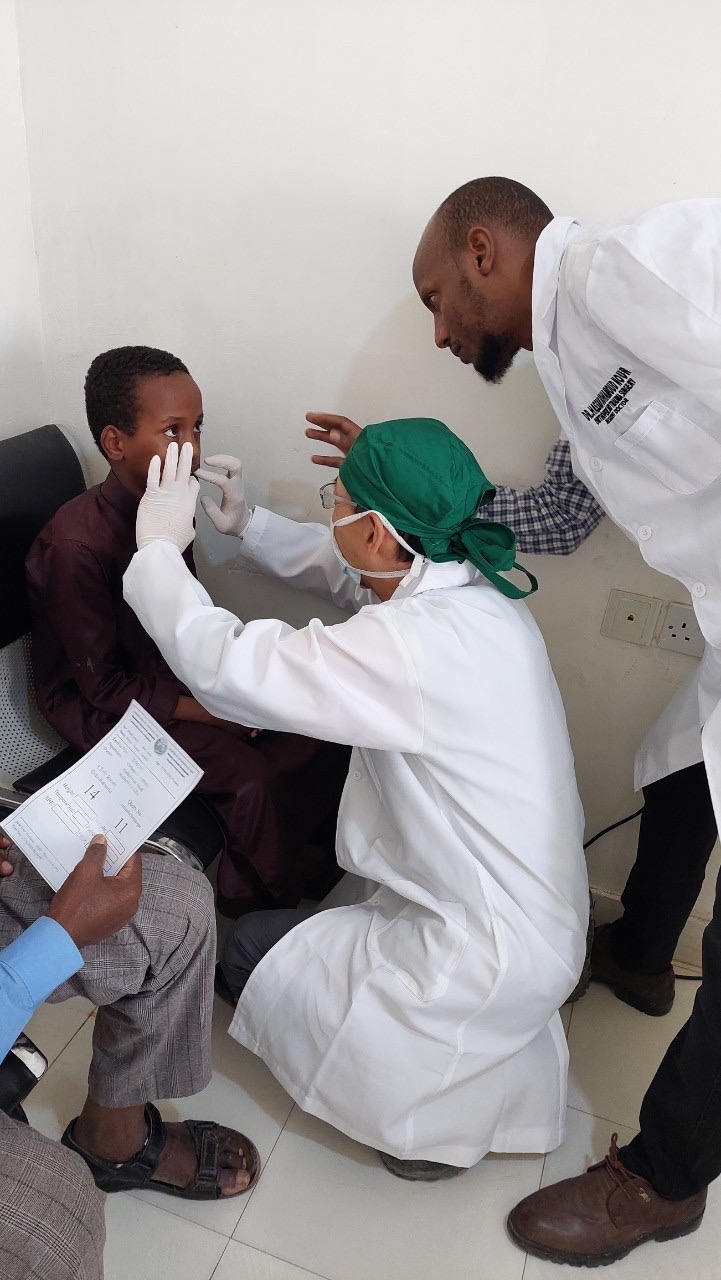
\includegraphics[width=0.24\textwidth]{IMG-4703.JPG}
        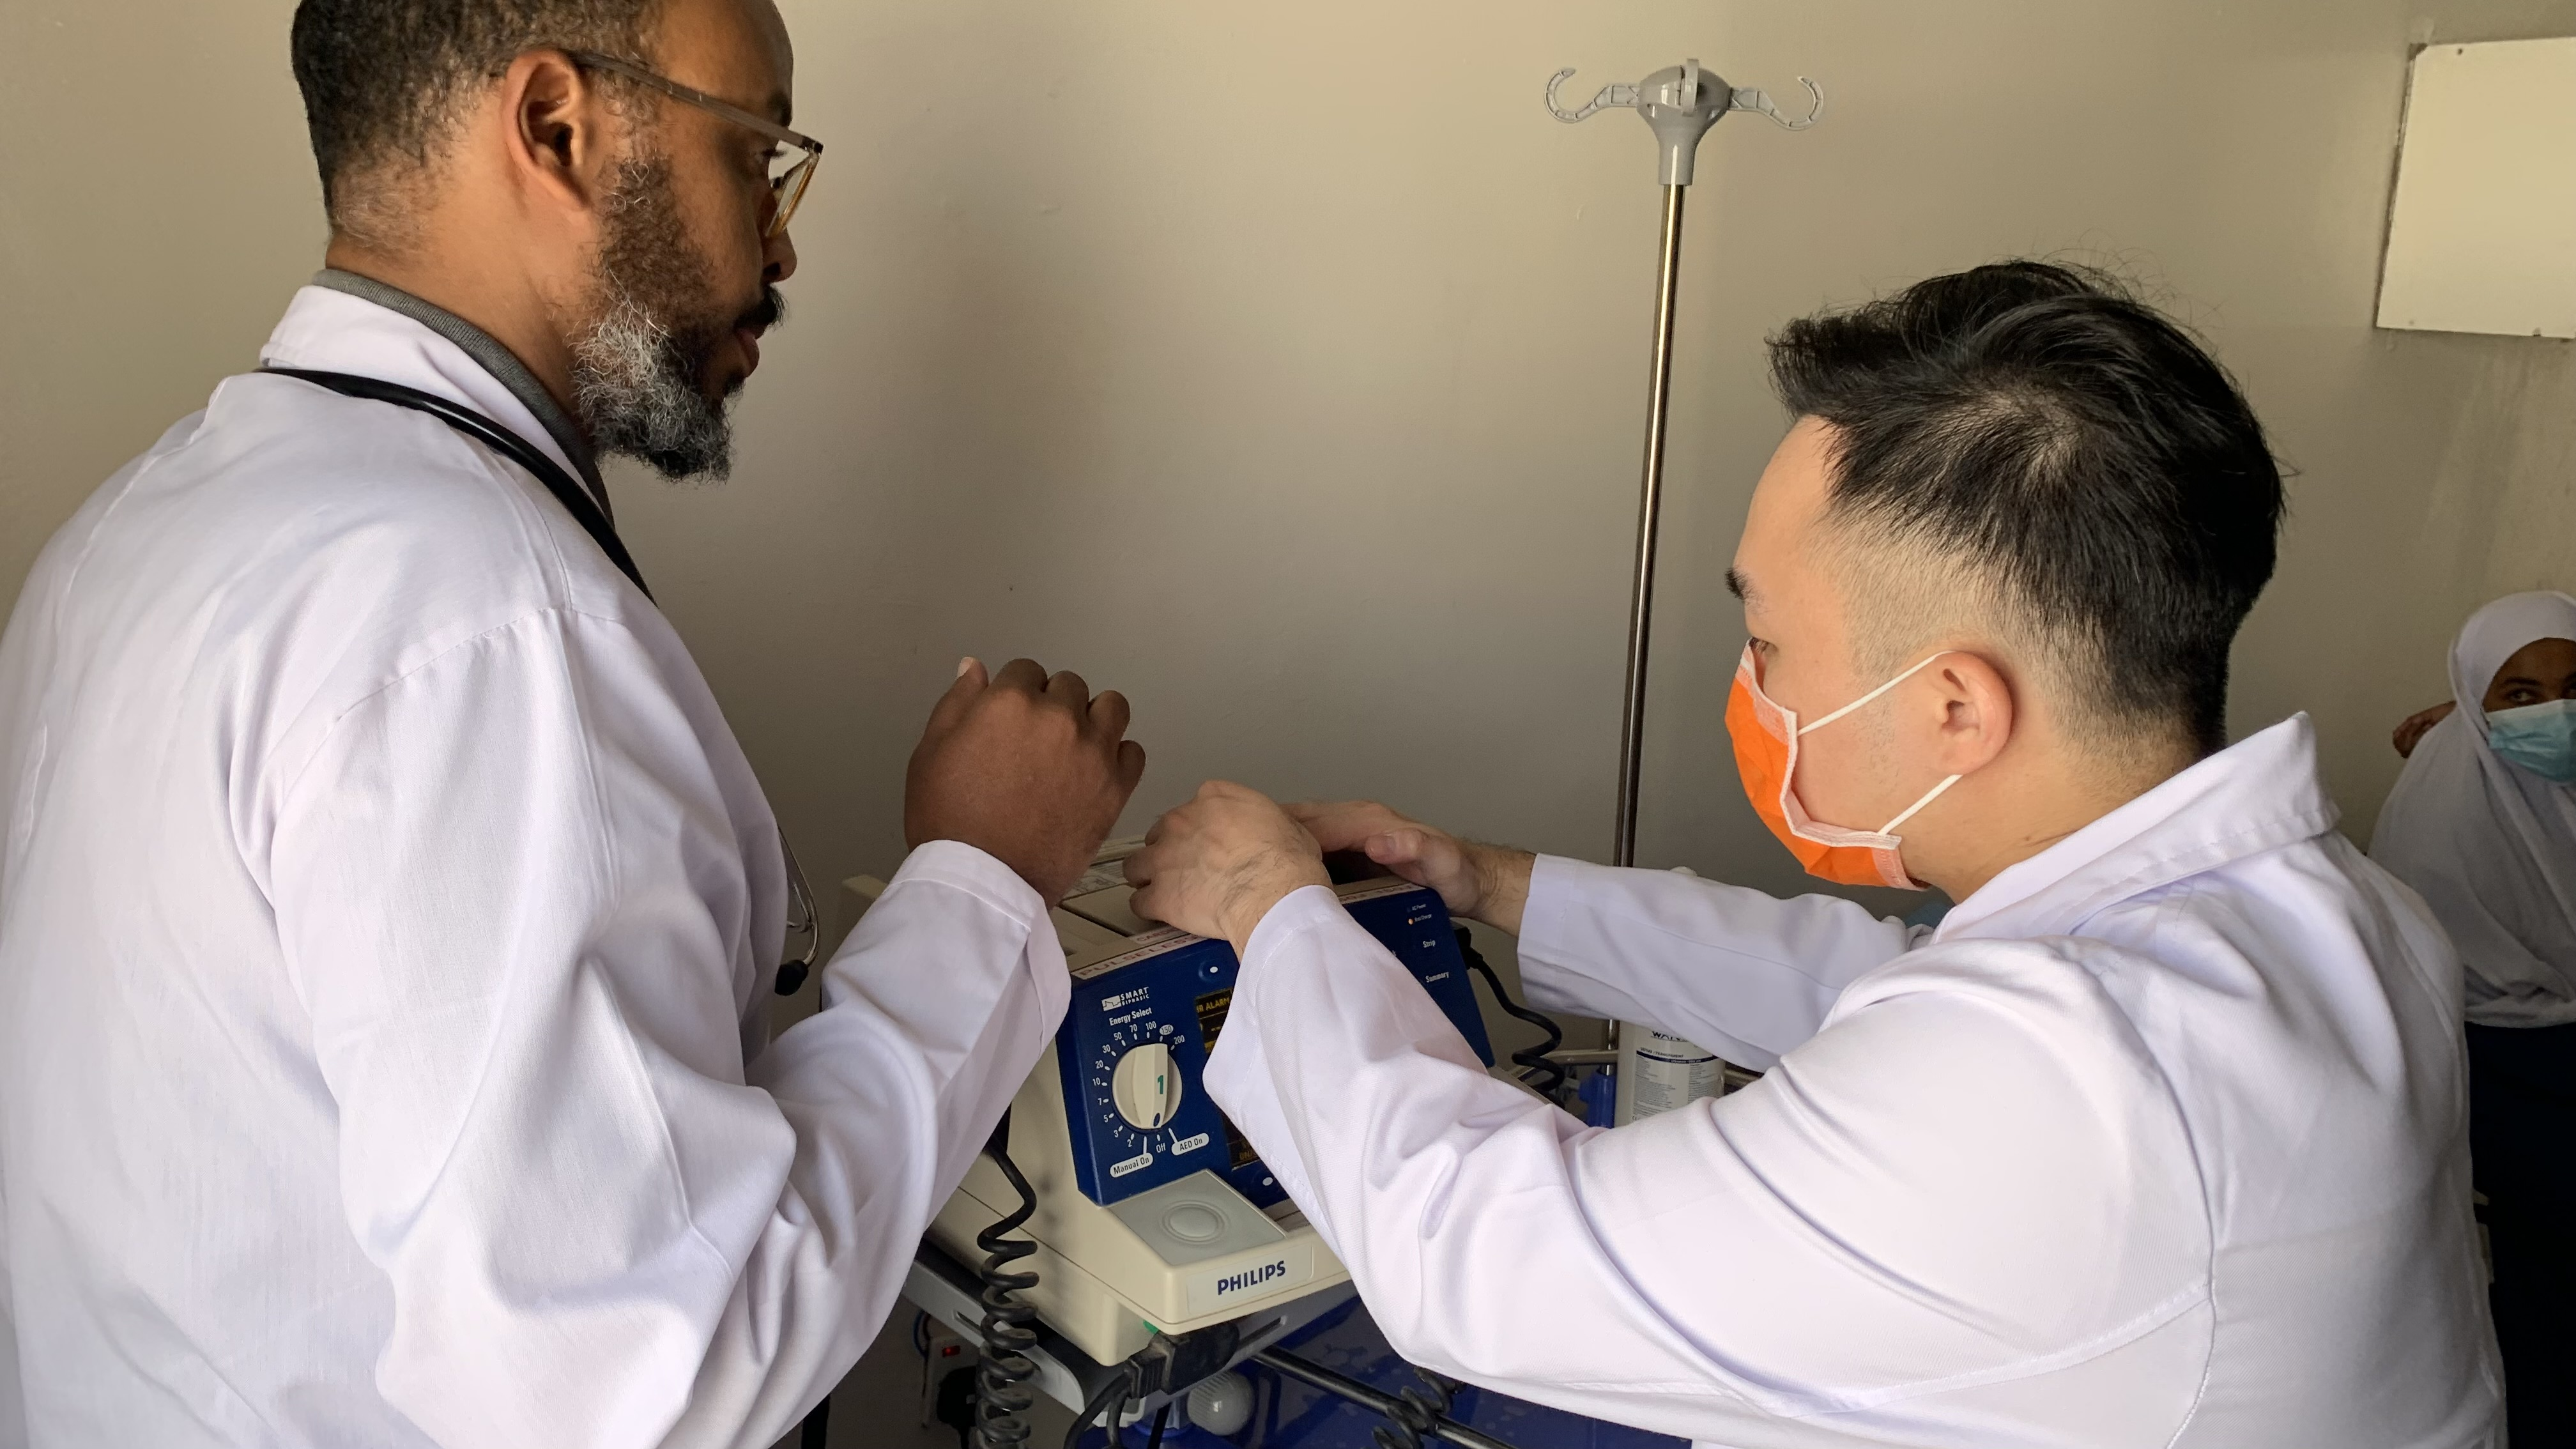
\includegraphics[width=0.24\textwidth]{IMG-5062.JPG}
        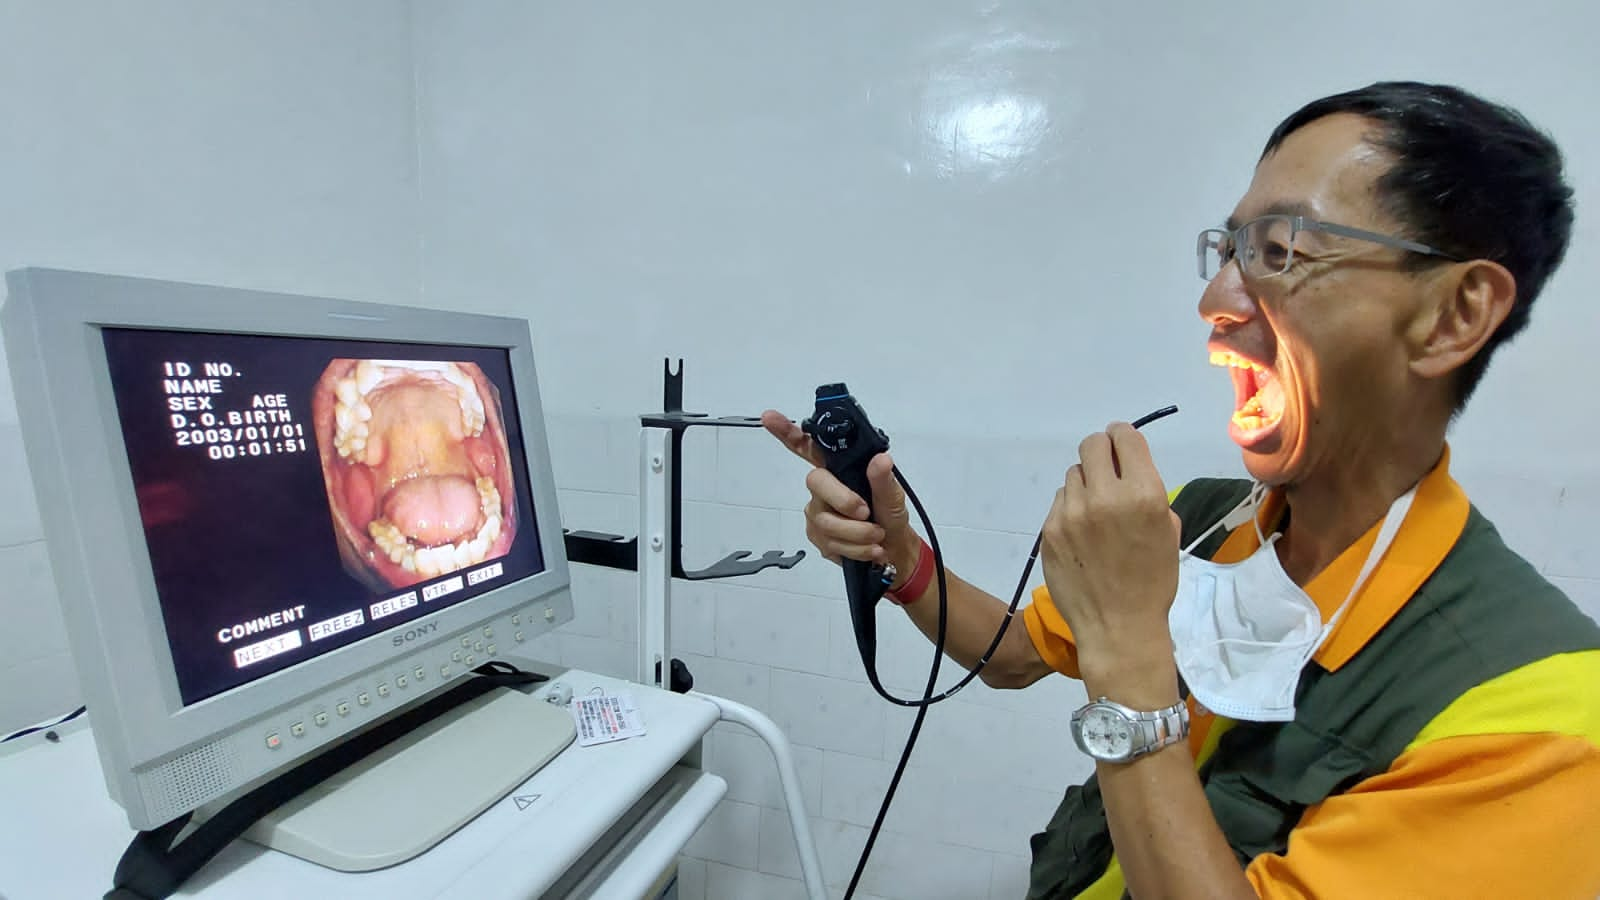
\includegraphics[width=0.24\textwidth]{6a625355-ae53-4e8f-891e-38a933f6c29b.JPG}    
    \end{center}
\end{frame}
%%    
\begin{frame}
\frametitle{TMM's Projects - third pillar}
% Add content here
\begin{outline}    
    \1 public health, we are launching
        \2 World Blood Donor Day campaign (2023/06/14)
        \2 Pap smear screen for elimination of cervical cancer (2023/07/11)
        \2 Good oral hygiene and oral cancer screening (March 2024)
        \2 HBV/HCV screenings, vaccinations, and treatment (2023/07/28)
        \2 Osteoprosis screening for women who get vitamin D deficience (Oct 2023)
        \2 Parasite screening program for schoolchildren (2024)
\end{outline}

\begin{center}
\includesvg[width=0.14\textwidth]{Blood_logo.svg}
\includesvg[width=0.14\textwidth]{anti_CervicalCancer_logo.svg}
\includesvg[width=0.22\textwidth]{World_OralHealth_Day_logo.svg}
\includesvg[width=0.14\textwidth]{WHD_logo.svg}
\includesvg[width=0.2\textwidth]{parasite_logo.svg}
\end{center}

\end{frame}

%%%

\begin{frame}{Oral health research}
\begin{outline}

Public health, we are studying
    \1 Exploring the Prevalence of \textcolor{red}{Halitosis and Tonsillitis} in Hargeisa Group Hospital, Somaliland: A Retrospective Pilot Study
        \2 Dr. Fadumo, Dr. Hersi, Dr. Omar, and Dr. Tex
    \1 Evaluating the Diagnostic Accuracy of CT-Scans and Serum Fluoride Levels in Detecting \textcolor{red}{Skeletal Fluorosis} in the Somaliland Population with \textcolor{red}{Dental Fluorosis}
        \2 Dr. Mukhtar, Dr. Fadumo, Dr. Ahmed Hashi, and Dr. Tex
    \1 \textcolor{red}{Deep Learning of Whole-slide images} in Oral Verrucous Hyperplasia
\end{outline}
    
\end{frame}


%%
\begin{frame}{Public health: Oral health}
    \begin{columns}
        
    \column{0.5\textwidth}
        \begin{center}
        \includesvg[width=0.7\textwidth]{World_OralHealth_Day_logo.svg}
            
        \end{center}
    \column{0.5\textwidth}
        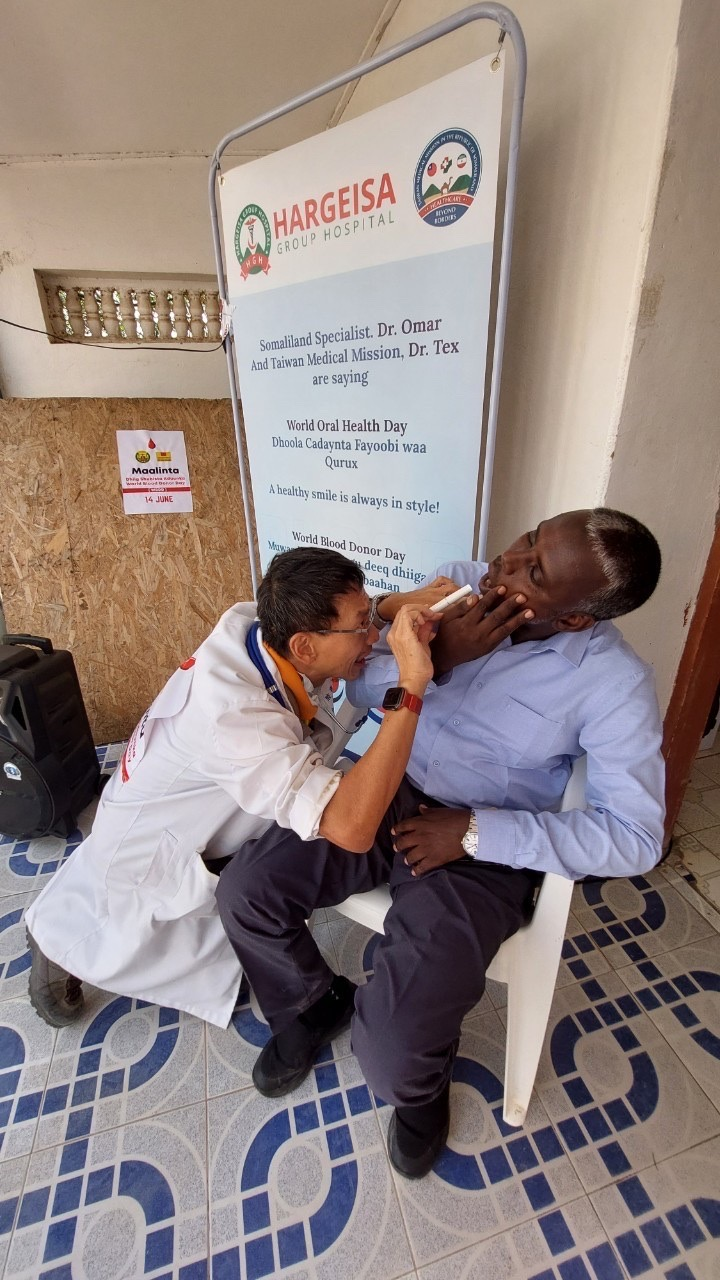
\includegraphics[width=0.7\textwidth]{IMG-4368.JPG}
%        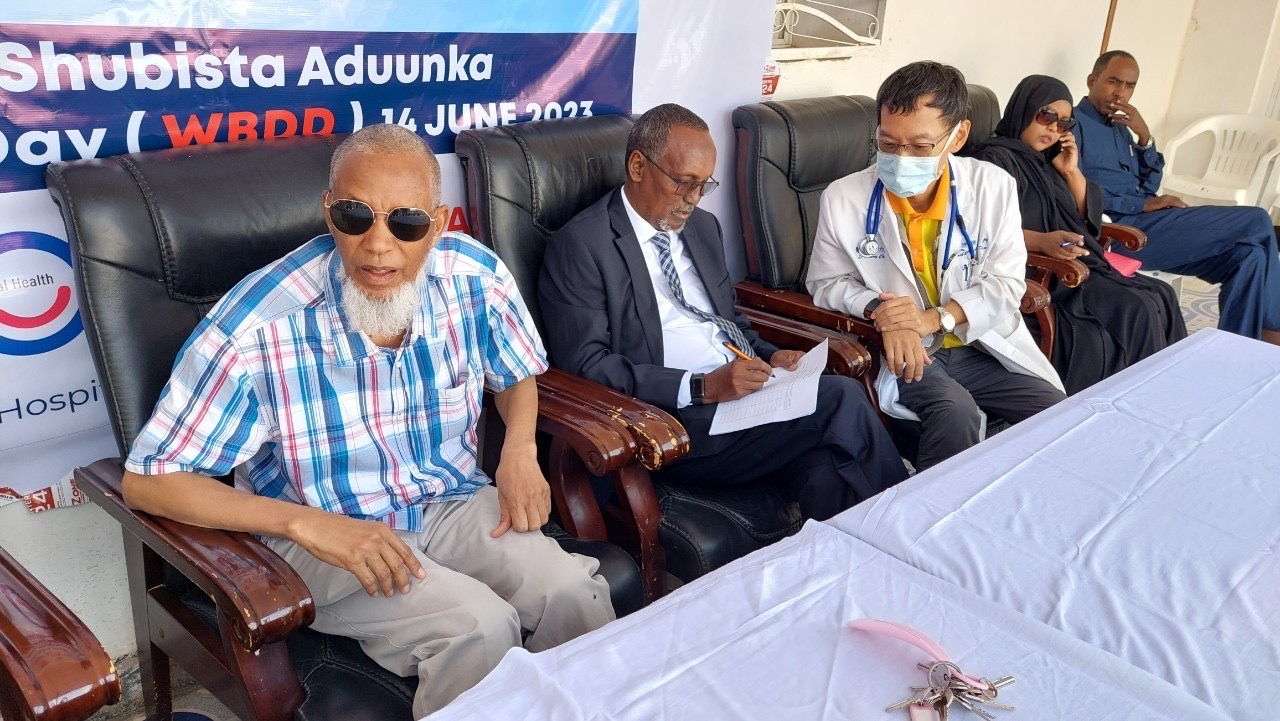
\includegraphics[width=0.45\textwidth]{IMG-4378.JPG}
    \end{columns}
\end{frame}




% Dr Askar
\begin{frame}{Public health: World Blood Donor Day}
    \begin{center}
        \includesvg[width=0.2\textwidth]{Blood_logo.svg}
%        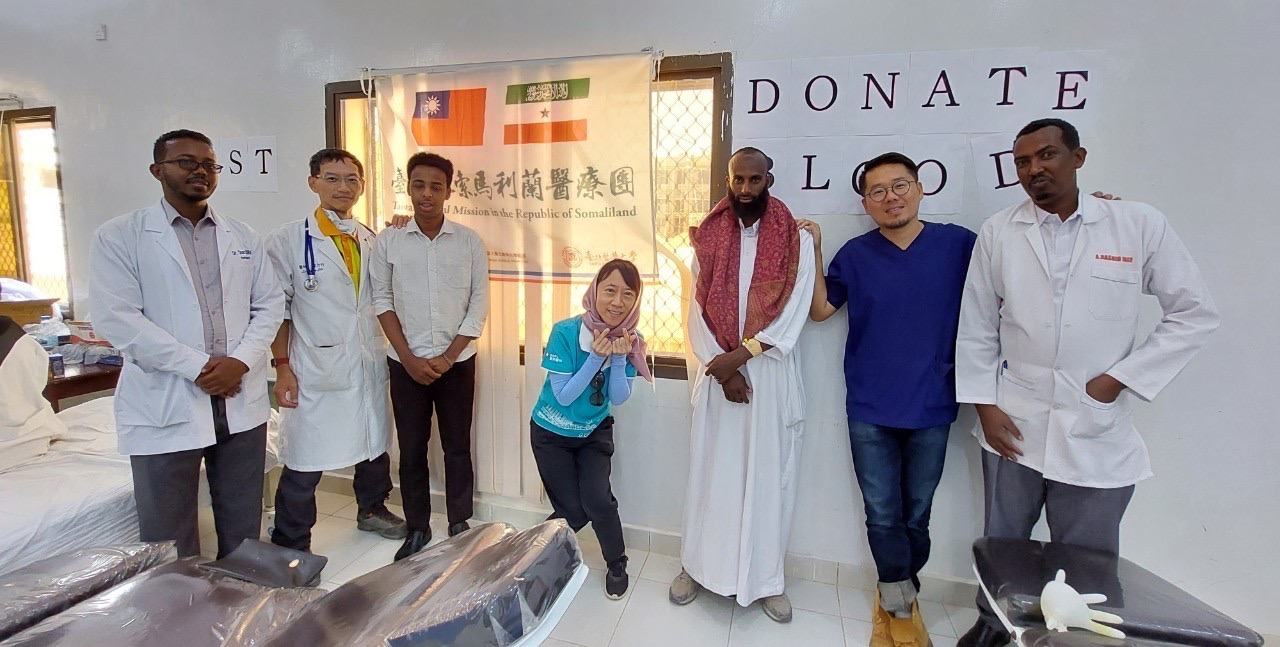
\includegraphics[width=0.35\textwidth]{IMG-4441.JPG}
        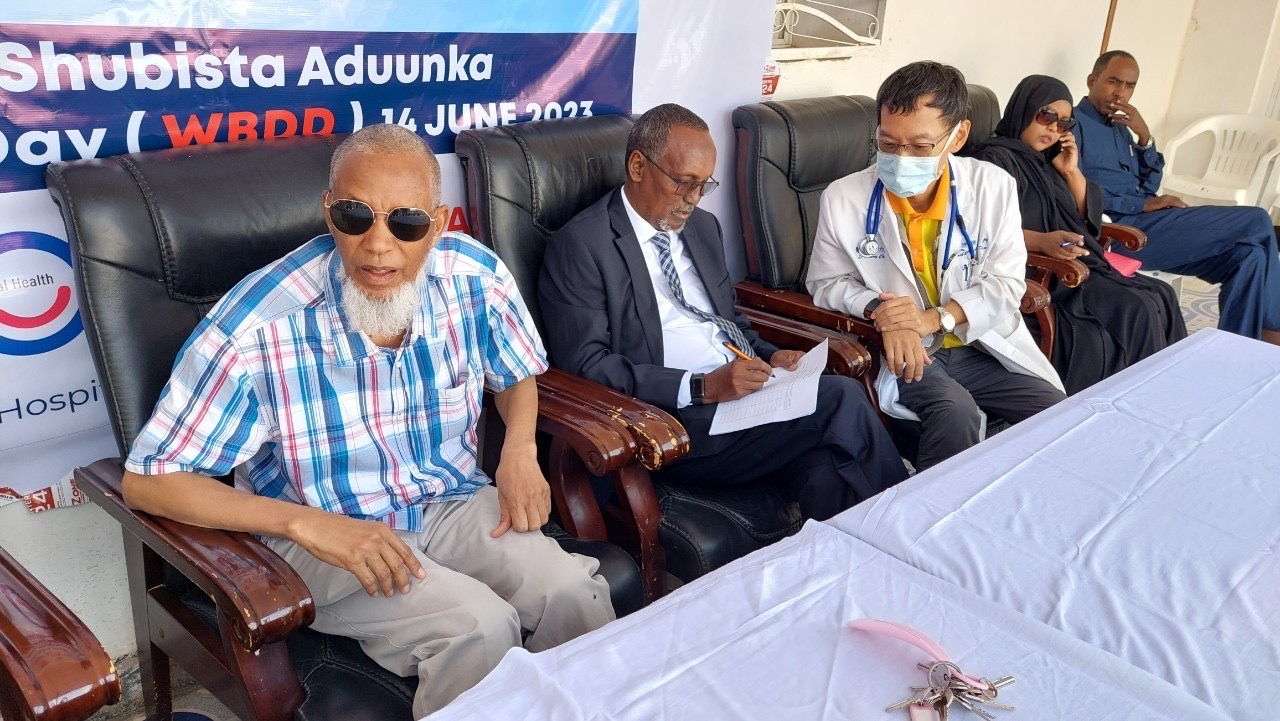
\includegraphics[width=0.75\textwidth]{IMG-4378.JPG}
    \end{center}
\end{frame}

% UoH student
\begin{frame}{Public health: World Blood Donor Day}
    \begin{center}
        \includesvg[width=0.2\textwidth]{Blood_logo.svg}
        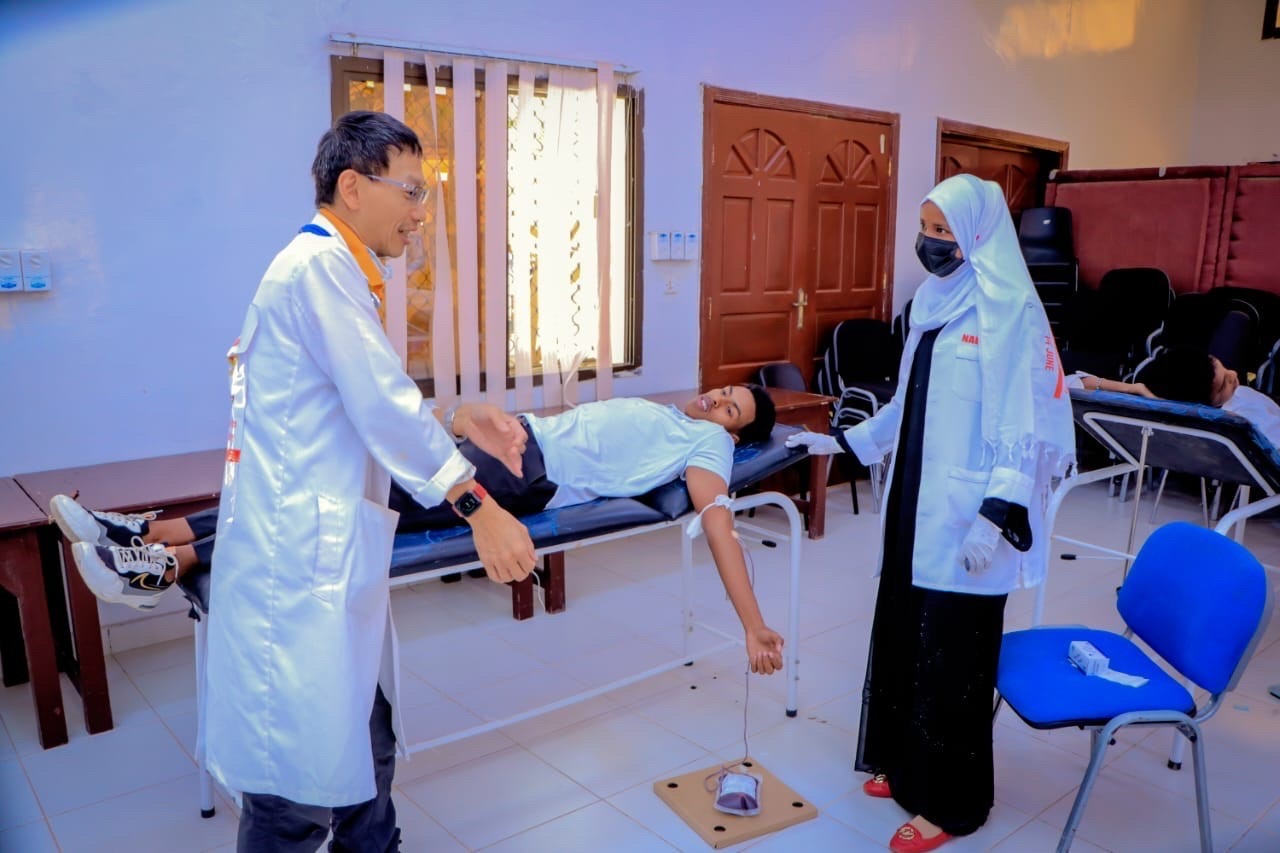
\includegraphics[width=0.45\textwidth]{IMG-5110.JPG}
        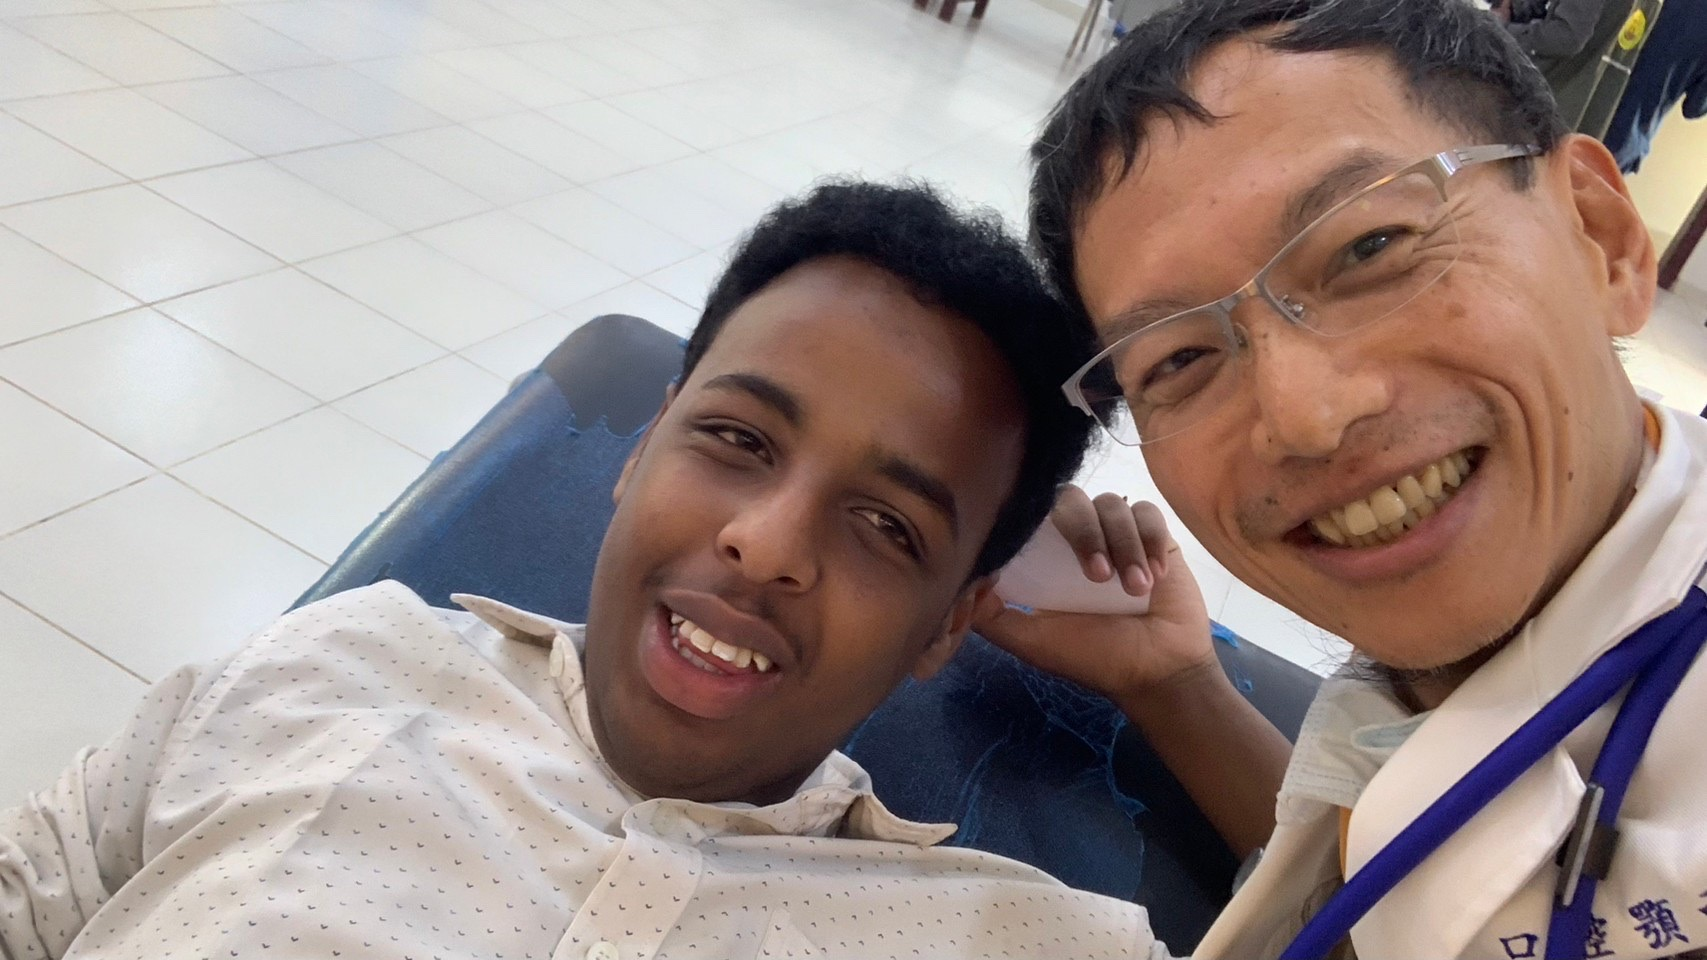
\includegraphics[width=0.25\textwidth]{IMG-5112.JPG}
    \end{center}
\end{frame}

\begin{frame}{Public health: World Blood Donor Day}
    \begin{center}
        \includesvg[width=0.2\textwidth]{Blood_logo.svg}
        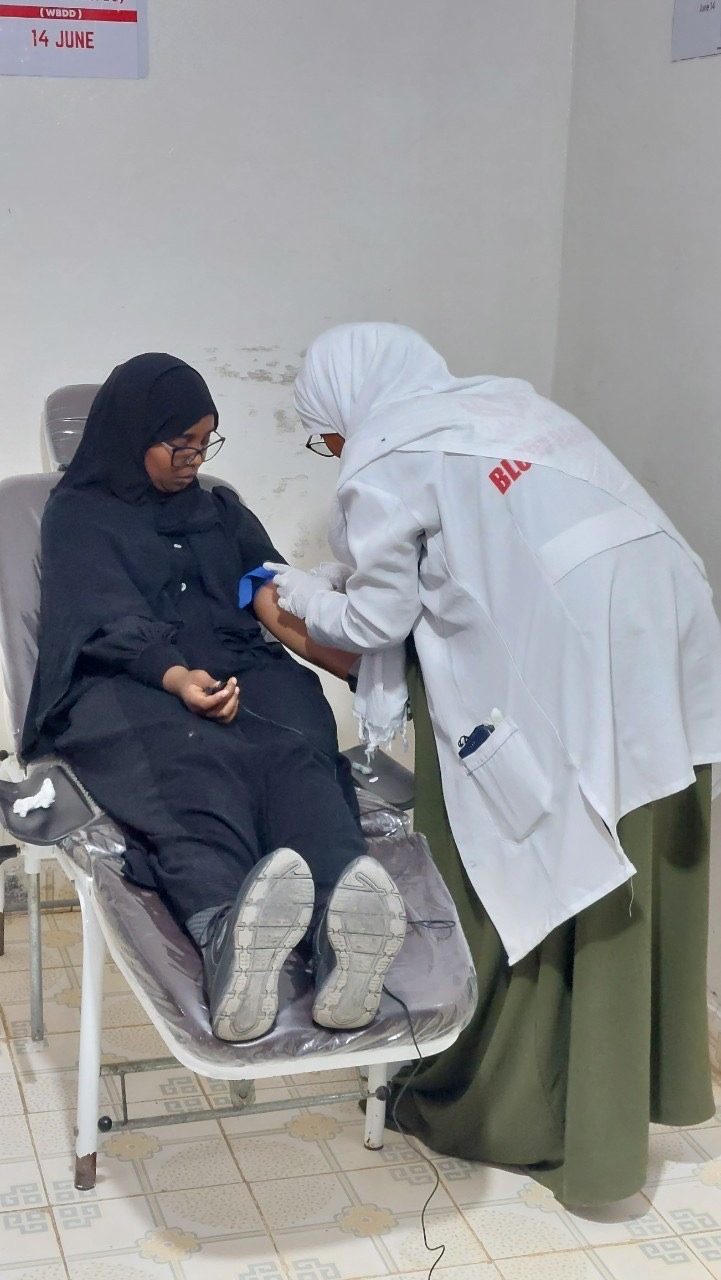
\includegraphics[width=0.30\textwidth]{IMG-4371.JPG}
        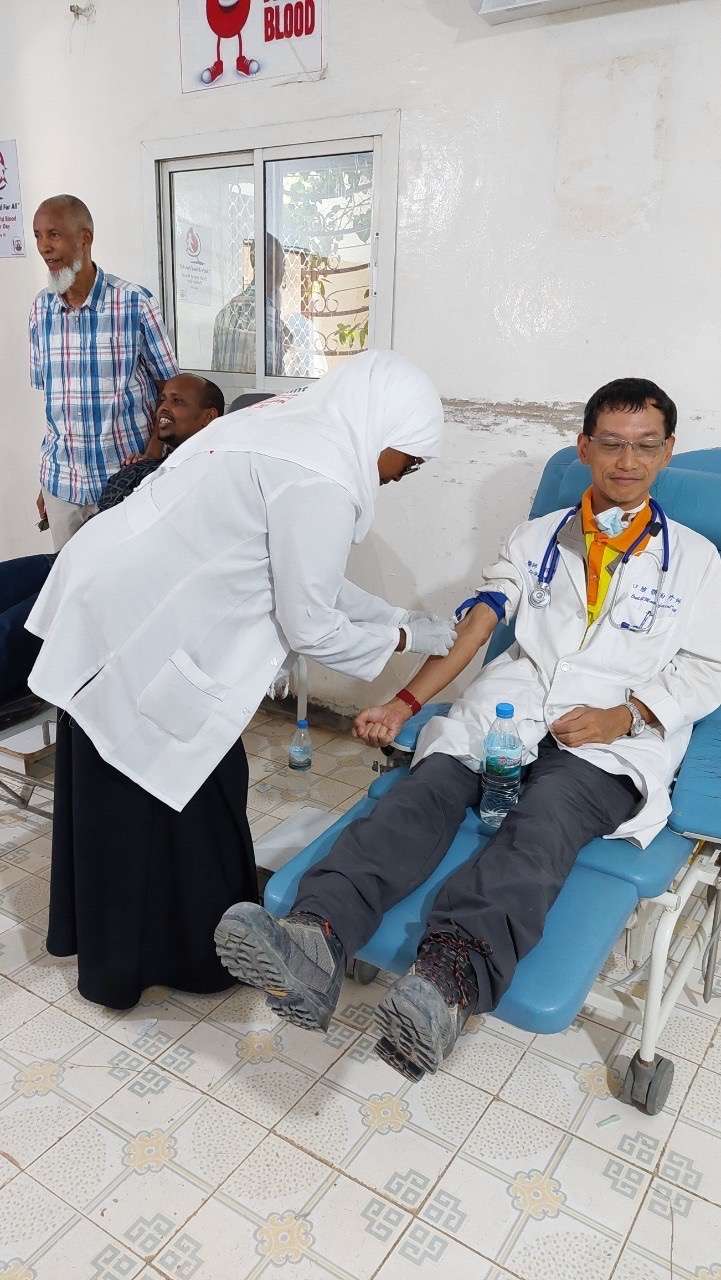
\includegraphics[width=0.30\textwidth]{IMG-4370.JPG}
    \end{center}
\end{frame}

\begin{frame}{Public health: World Blood Donor Day}
    \begin{center}
        \includesvg[width=0.2\textwidth]{Blood_logo.svg}
        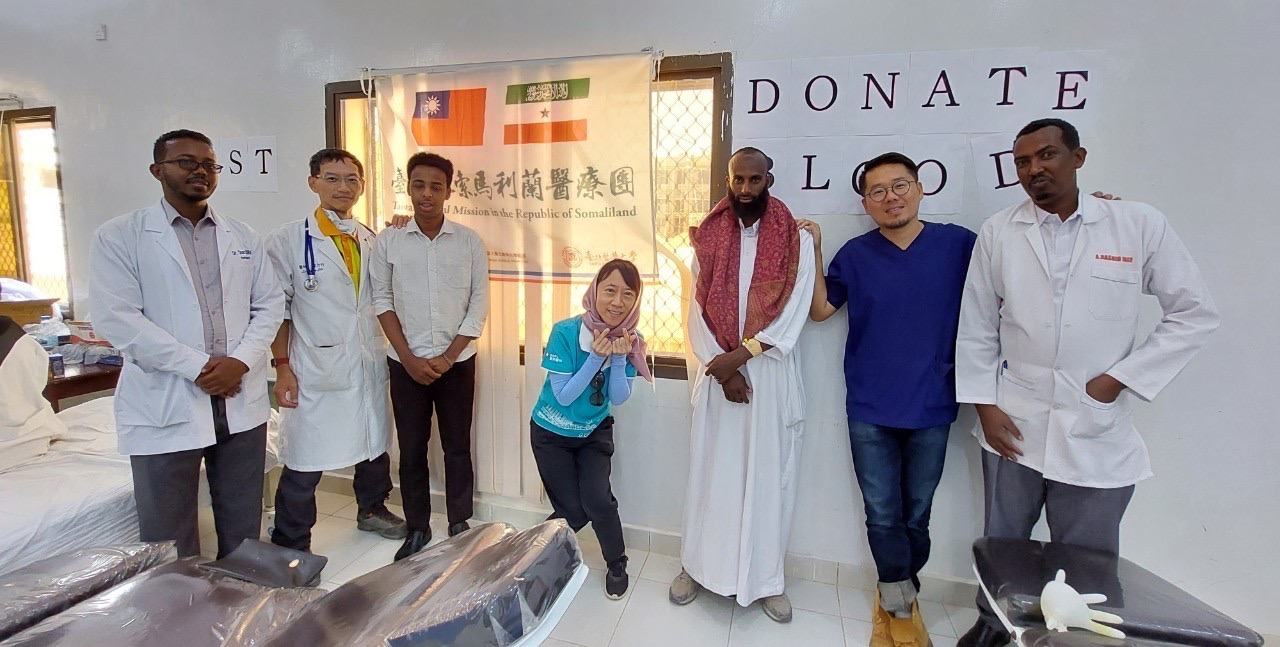
\includegraphics[width=0.75\textwidth]{IMG-4441.JPG}
%        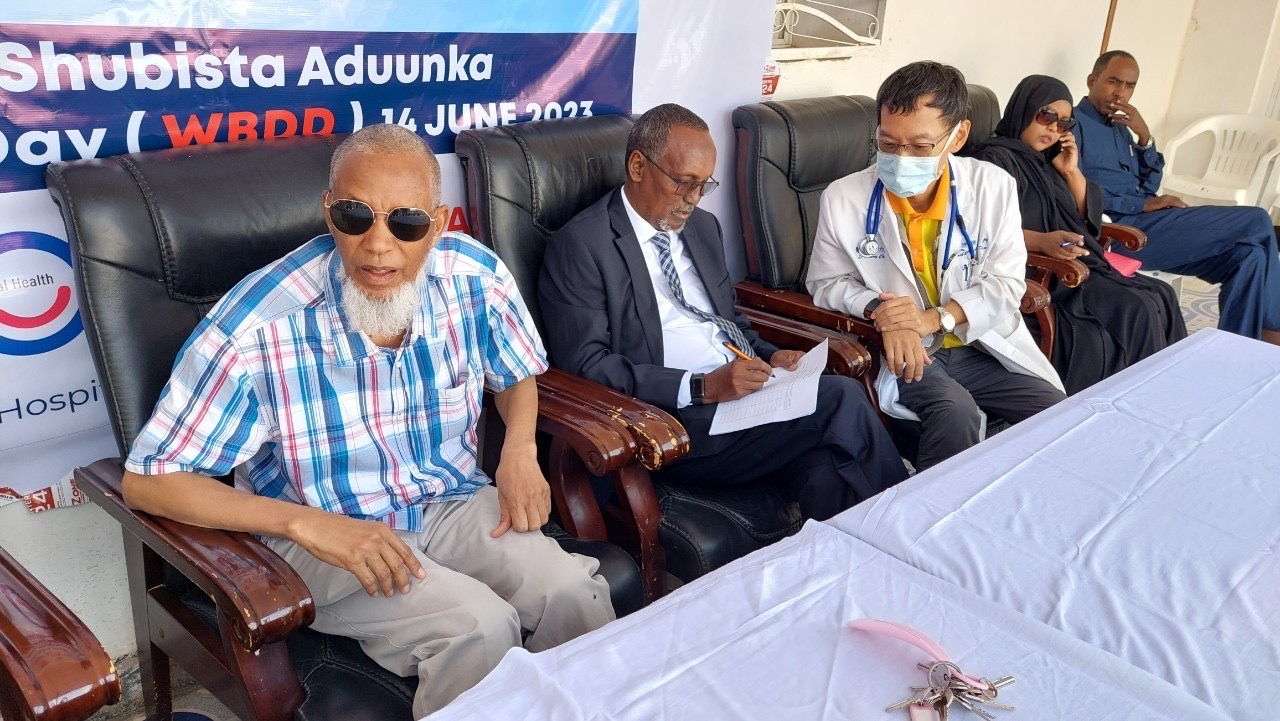
\includegraphics[width=0.45\textwidth]{IMG-4378.JPG}
    \end{center}
\end{frame}


\begin{frame}{Public health: Pap smear program since 2023/07/11}
    \begin{center}
        
\includegraphics[width=4.5cm, height=6.5cm]{IMG-5434.JPG} 
        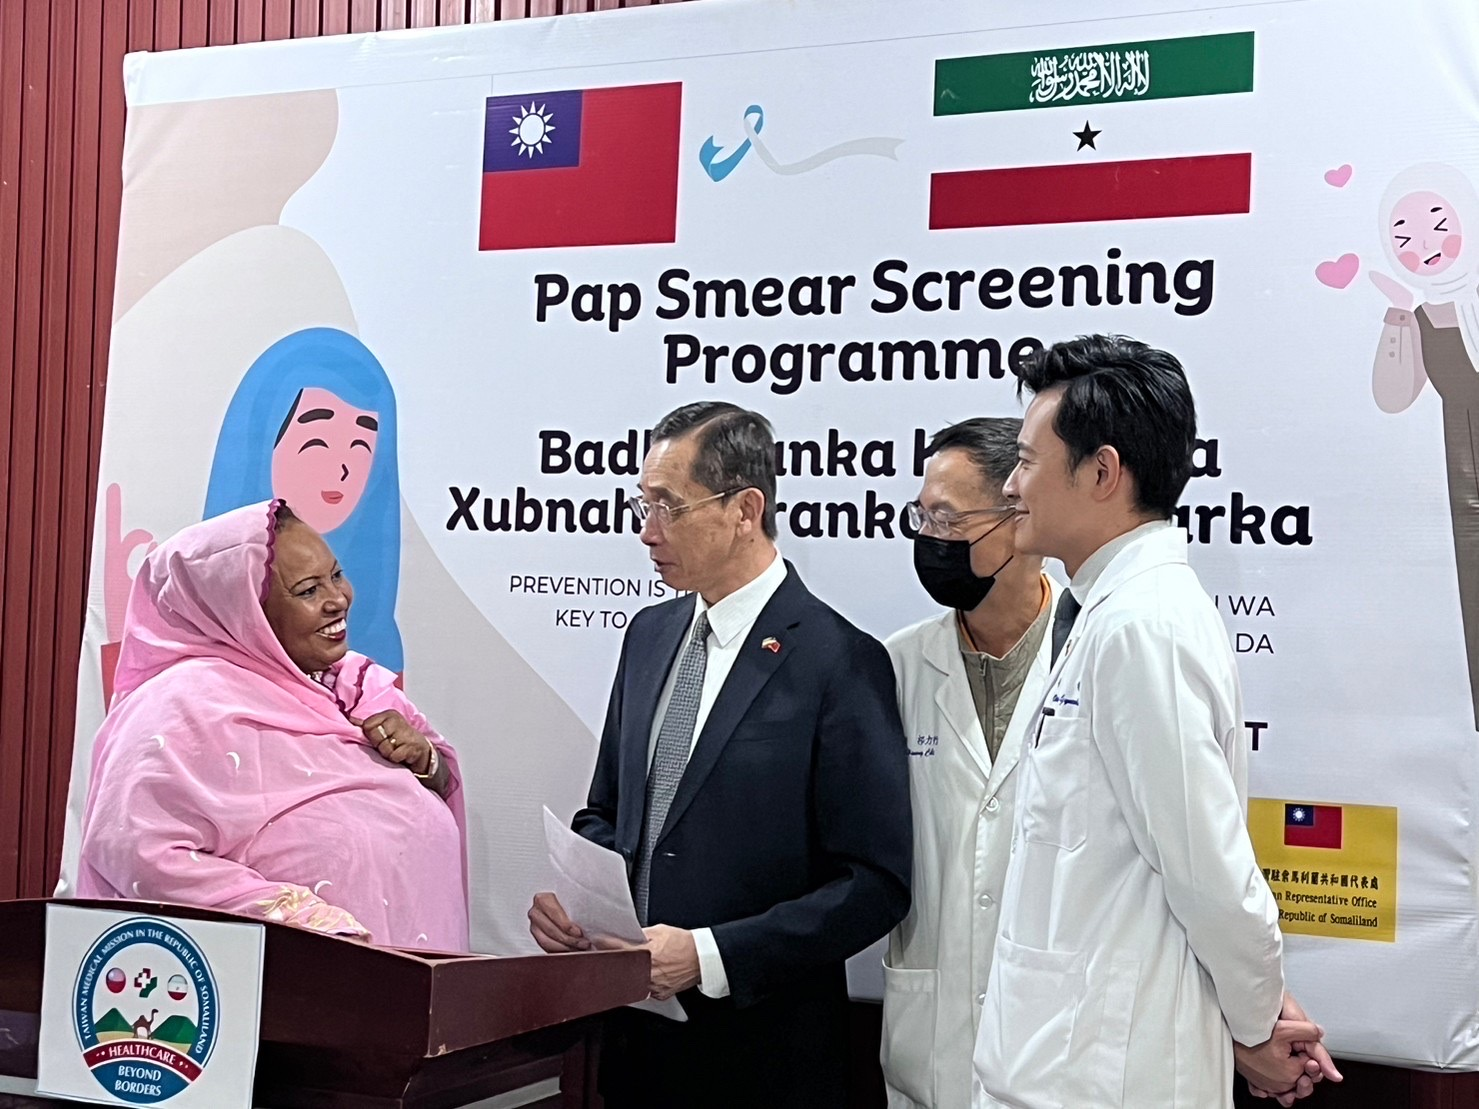
\includegraphics[width=0.6\textwidth]{IMG-5436.JPG}
%        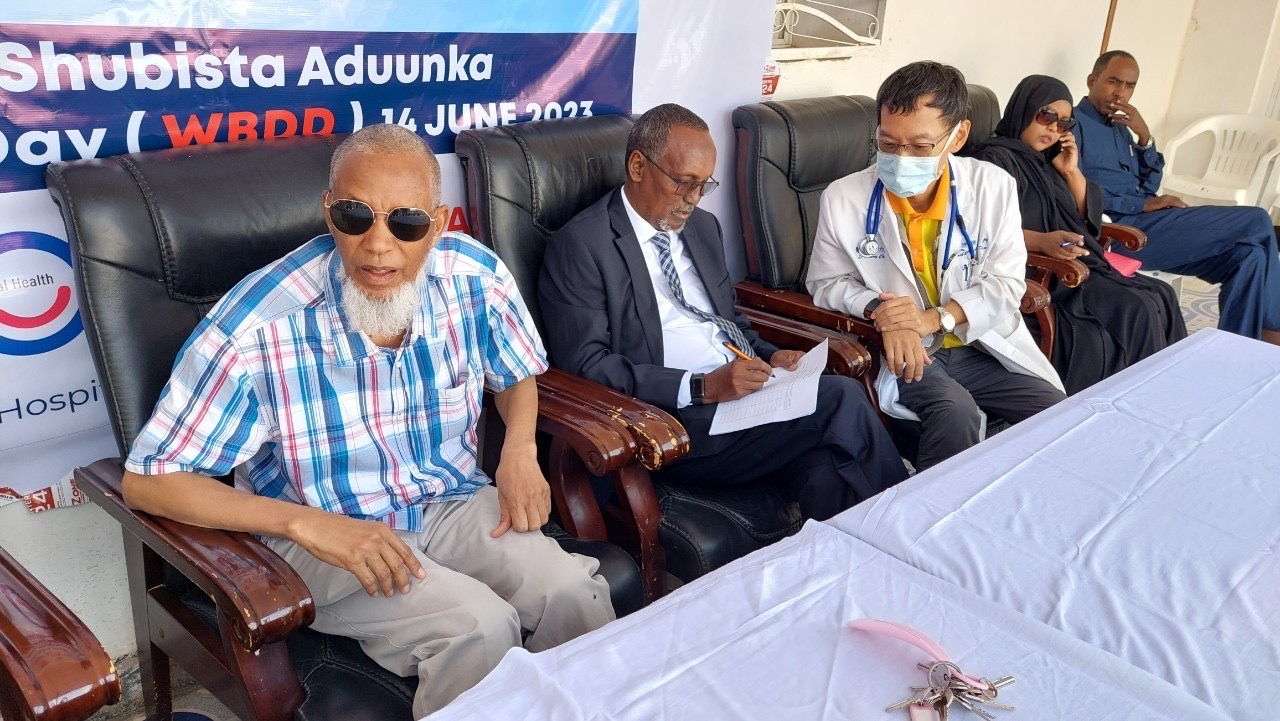
\includegraphics[width=0.45\textwidth]{IMG-4378.JPG}
    \end{center}
\end{frame}


\begin{frame}{Public health: Pap smear program (Dr. Dave Lin)}
    \begin{center}
%        \includesvg[width=0.2\textwidth]{Blood_logo.svg}
        \includegraphics[width=0.95\textwidth]{IMG-5437.JPG}
%        \includegraphics[width=0.45\textwidth]{IMG-4378.JPG}
    \end{center}
\end{frame}
%%%

\begin{frame}
\frametitle{TMM's Projects - fourth pillar}
% Add content here
\begin{outline}    
    \1 telemedicine
        \2 by collaborating with specialists at TMU affiliated Hospitals
        \2 \textcolor{red}{telepathology} project with a pathologist through digital whole-slide images (WSIs)
        \2 \textcolor{red}{"RadiPush"} project to fasciliate last-mile transfer of radiologist reports to doctors; for example: Taiwan Osteoporosis Master for T-score
    
\end{outline}
\end{frame}


\begin{frame}{Telepathology and Radiology}
    \begin{center}
        \includegraphics[width=0.35\textwidth]{TH1919729C1_HE.jpeg}
        \includegraphics[width=0.30\textwidth]{IMG-0007-00001.jpg}
    \end{center}
\end{frame}


\begin{frame}{Teleconsultation: non-human vertebrae (cheetah)}
    \begin{center}
        \includegraphics[width=0.35\textwidth]{457256160987709682.jpg}        \includegraphics[width=0.35\textwidth, origin=c,angle=180]{IMG-5116.JPG}

    \end{center}
\end{frame}

%%%%%%%%%%%%%%%%5555

\begin{frame}{2023/07 Laas Geel, Somaliland}
    \begin{center}
        \includegraphics[width=1.0\textwidth]{IMG-5232.jpg}
        %\includegraphics[width=0.85\textwidth, origin=c,angle=180]{IMG-5116.JPG}

    \end{center}

\end{frame}


\begin{frame}{2023/07 Laas Geel, Somaliland}
    \begin{center}
        \includegraphics[width=0.25\textwidth]{IMG-5205.jpg}
        \includegraphics[width=0.55\textwidth]{IMG-5247.jpg}

    \end{center}

\end{frame}


\begin{frame}{7000-year-old tales}
    \begin{center}
        \includegraphics[width=0.45\textwidth]{IMG-5204.jpg}
        \includegraphics[width=0.45\textwidth]{IMG-5226.jpg}

    \end{center}

\end{frame}

%%%%%%%%%%%%%

\section{Somaliland's Stories}

\begin{frame}{Somaliland patient stories}
    \begin{center}
    \includesvg[width=0.35\textwidth]{TMWH_logo_TAIPEI_vector.svg} 
    \includesvg[width=0.45\textwidth]{Hargeisa_Group_Hospital_logo(1).svg} 
%    \includegraphics[width=0.3\textwidth, trim=60mm 60mm 30mm 60mm,clip]{52165_antenatal_check.jpg}

\end{center}
\end{frame}

%% ultrasound baby
\begin{frame}
\frametitle{Nimco, happy mother first "see" her baby}
% Add content here
\begin{center}
    \includegraphics[width=0.3\textwidth, trim=00mm 100mm 00mm 60mm,clip]{IMG-5117.JPG} 
    \includegraphics[width=0.3\textwidth, trim=60mm 60mm 30mm 60mm,clip]{52165_antenatal_check.jpg}

\end{center}
\end{frame}

%% Ismail oral cancer
\begin{frame}
\frametitle{Ismail said, "Welcome, I'm going to sleep."}
% Add content here
\begin{center}
\raisebox{70mm}{
    \includegraphics[width=0.8\textwidth, scale=-1,angle=180]{IMG-4861.jpg} 
    }
%    \includegraphics[width=0.3\textwidth, trim=60mm 60mm 30mm 60mm,clip]{52165_antenatal_check.jpg}

\end{center}
\end{frame}

%%%%%%%%%%
\section{Conclusion}
\begin{frame}
\frametitle{Thanks all of TMM members (2022, 2023, 2024, ...)}
% Add content here
\begin{center}
\raisebox{90mm}{
    \includegraphics[width=0.5\textwidth]{IMG-5017.JPG} 
    \includegraphics[width=0.5\textwidth]{IMG-5437.JPG} 
    }
%    \includegraphics[width=0.3\textwidth, trim=60mm 60mm 30mm 60mm,clip]{52165_antenatal_check.jpg}

\end{center}
\end{frame}


%%
\begin{frame}
\frametitle{Take Home Message}
% Add content here
\begin{columns}
    
\column{0.4\textwidth}


\begin{outline}
 %   Our core value is:
我們正在撰寫索蘭的醫療史
\1 教學
\1 服務
\1 公衛

%\1 TMM offers medical professionals for people in need.
%\1 TMM's presence is supposed to bring happiness and safety to everyone around them
%iby improving their health and well-being.
%\1 TMM members have confidence, resilience, determination, and empathy when they face challenges.
\end{outline}

\column{0.6\textwidth}
\includegraphics[width=0.6\textwidth]{IMG-0394.JPG}
\end{columns}
\end{frame}

\begin{frame}{Trust me, Trust you}

\begin{columns}
    
\column{0.4\textwidth}
\begin{outline}
%Whenever TMM's members have short-term or long-term work in Somaliland,

\1 A chief doctor in TMM (Ph.D. of \textcolor{red}{Translational Medicine}, Master of \textcolor{red}{ Biomedical Informatics}; deep learning AI physician scientist):
    \2 教學
    \2 服務
    \2 公衛/\textcolor{red}{研究}

%\1 TMM members work as a team in Somaliland, whether they are there for a short time or for a long time.
\1 You can, however, think about how you can use the skills and experiences \textcolor{red}{you gained} here in your future job and life in Taiwan.
%\1 You can make the most of this time as a chance to learn and grow so that you can help us all get
%through \textcolor{blue}{the challenges} that we face here. 
%\1 We think that constant help is important for our overseas mission to be successful.

\end{outline}

\column{0.6\textwidth}
\includegraphics[width=0.7\textwidth]{IMG-5113.JPG}
\end{columns}

\end{frame}
%%

\begin{frame}{Outreach}
    \begin{columns}
    to community (IDP site C)
    \column{0.6\textwidth}
    \includegraphics[width=0.7\textwidth]{IMG_1713.jpeg}
    \end{columns}  
\end{frame}


%%%
\begin{frame}{Finale}
\begin{columns}
    
\column{0.4\textwidth}
\qrcode[height=2in]{https://www.facebook.com/profile.php?id=100094220689116&mibextid=LQQJ4d}
TMM facebook

\column{0.6\textwidth}
TMU白袍下的熱血---續集2024
\begin{outline}


    \1 人性面的溫暖,包容現實層面的無能為力
        \2 看病實況:一切自費,好似 1973 年代的臺灣
        \2 "他們"比起"我們"更能坦然接受死亡
        \2 \textcolor{red}{因為沒有很多,所以能捨}
    \1 當個非洲醫師的經驗,真好
%娓娓道來 

\end{outline}


\end{columns}
\end{frame}


%\end{CJK*}

\end{document}
